%----------------------------------------------------------------------------------------
%	PACKAGES AND OTHER DOCUMENT CONFIGURATIONS
%----------------------------------------------------------------------------------------

\documentclass[twoside,openright,12pt,fleqn]{book}
%\special{papersize=210mm,297mm}
\linespread{1.15} % Line spacing - Palatino needs more space between lines
\usepackage{microtype} % Slightly tweak font spacing for aesthetics

% leave 10pt blank space between paragraphs
\usepackage[skip=10pt plus1pt, indent=0pt]{parskip}	

% Used for blank pages
\usepackage{afterpage}
\newcommand\blankpage{
    \null
    \thispagestyle{empty}
    \addtocounter{page}{-1}
    \newpage}

%geometry and layout
\pagestyle{plain} % center all page numbering
\usepackage[
	letterpaper,
	inner=30mm,
	outer=25mm,
	bottom=21.5mm,
	footskip=13.5mm	
]{geometry} % paperstyle and margins
\voffset -14mm
%\headsep 14mm


\usepackage{multicol} % Used for the two-column layout of the document
\usepackage[hang, font=small,labelfont=bf,up]{caption} % Custom captions under/above floats in tables or figures
\usepackage{booktabs} % Horizontal rules in tables
\usepackage{float} % Required for tables and figures in the multi-column environment - they need to be placed in specific locations with the [H] (e.g. \begin{table}[H])

%\usepackage{lettrine} % The lettrine is the first enlarged letter at the beginning of the text
\usepackage{paralist} % Used for the compactitem environment which makes bullet points with less space between them

\usepackage{titlesec} % Allows customization of titles
\renewcommand\thesection{\Roman{section}} % Roman numerals for the sections
\renewcommand\thesubsection{\Roman{subsection}} % Roman numerals for subsections
\titleformat{\section}[block]{\large\scshape}{\thesection.}{1em}{} % Change the look of the section titles
\titleformat{\subsection}[block]{\large}{\thesubsection.}{1em}{} % Change the look of the section titles
\newcommand\abstractfont{\fontsize{11pt}{10pt}\selectfont} % specific font for abstract
\titleformat{\chapter}[block]
	{\bfseries\huge}{\filright\huge\thechapter\hspace{1ex}\textnormal{|}}{1ex}{\huge\filright }
% JS packages
\usepackage{etex}
\usepackage{tabto}
\usepackage{paralist}

%\usepgfmodule{plot}
\usepackage{xcolor}
\usepackage{graphicx}
\usepackage{setspace}
\usepackage{textcomp}


\usepackage{amsmath}
\usepackage{lmodern}
\usepackage{listings}
\usepackage[numbered,framed]{matlab-prettifier}
\usepackage{subcaption}
\usepackage{textcomp}
%\usepackage{txfonts}
\usepackage{geometry}
\usepackage{nameref}
\usepackage[finalnew]{Stylesheets/trackchanges}
\usepackage[colorlinks=true]{hyperref} % For hyperlinks in the PDF

% settings bibliography
\usepackage[round]{natbib}
\usepackage{bibentry}
\nobibliography* % suppresses bibliography mention for bibentry commands

% for figures: caption , subcaption
\captionsetup[figure]{labelformat=simple, labelsep=colon, textfont=normalfont, font=footnotesize} %{stretch=1.1}
%\captionsetup[table]{labelformat=simple, labelsep=colon, textfont=normalfont}
%\captionsetup[subfigure]{labelformat=simple, labelsep=colon, textfont=normalfont}

\renewcommand{\thesection}{\arabic{section}}%... from subsections
\renewcommand{\thesubsection}{\arabic{section}.\arabic{subsection}}%... from subsections
\renewcommand{\thesubsubsection}{\arabic{section}.\arabic{subsection}.\arabic{subsubsection}}%... from subsections

\definecolor{light-gray}{gray}{0.8}
\graphicspath{{./Images/}}

\def\degr{${}^\circ$}

%----------------------------------------------------------------------------------------
%	TITLE SECTION
%----------------------------------------------------------------------------------------
\title{\vspace{-15mm}\fontsize{24pt}{10pt}\selectfont\textbf{}} % Article title

\author{
\large
%\textsc
{Margot Mangnus$^1$}\\[2mm] % Your name
\small $^1$ Donders Institute for Brain, Cognition and Behaviour, Radboud University Nijmegen, The Netherlands\\ % Your institution
%\normalsize \href{mailto:}{} % Your email address
\vspace{-5mm}
}
\date{\today}

%----------------------------------------------------------------------------------------
% BEGIN DOCUMENT
%----------------------------------------------------------------------------------------

\renewcommand{\familydefault}{\sfdefault}
%\usepackage[default,osfigures,scale=0.95]{Open Sans}
\usepackage[T1]{fontenc}
%\normalfont
\usepackage[sfdefault]{AlegreyaSans} 

\begin{document}
\setlength{\parindent}{0.5pt}
%\thispagestyle{fancy} % All pages have headers and footers
\renewcommand{\vec}[1]{\mathbf{#1}} %This command will make \vec typeset LaTeX vectors using bold instead of an arrow:

\begin{titlepage}
	\centering
	\vspace{1cm}
	\vspace{1.5cm}
	{\huge\bfseries When Communication is Hard: \\ Neurocognitive Dynamics underlying \\ Language and Communication \\in Autism and Social Anxiety \par}	%into the cortical depths of the unknown
	\vspace{4cm}
	{\Large by \\ Margot Mangnus \par}
	\vfill
\end{titlepage}

%% first title page
\thispagestyle{empty}

{\setlength{\parindent}{0cm}
	\begin{flushright}
		\vspace{120pt}
		\huge{On the analysis of layer-specific fMRI}\\
		\vspace{80pt}
		\large{Tim van Mourik}
	\end{flushright}
}

\newpage

% metadata page, 
\thispagestyle{empty}
{\setlength{\parindent}{0cm}\raggedright\smaller
\null\vfill

The work described in this thesis was carried out at the Donders Institute for Brain, Cognition, and Behaviour, Radboud University Nijmegen, with financial support from the NWO Spinoza Prize (SPI 40-118) awarded to prof. dr. Peter Hagoort.

\vspace{12pt}

\textbf{ISBN/EAN: 978-94-6284-167-3}

\vspace{12pt}
\textbf{Design \& layout}\\
Michel Wolf, mw:ontwerp, Nijmegen

\vspace{12pt}
Copyright {\textcopyright} Tim van Mourik, 2018. 
}

\newpage

% official Dutch title page
\thispagestyle{empty}
\begin{minipage}[c]{100mm}

\begin{center}
\vspace{20pt}
\large{\textbf{On the analysis of layer-specific fMRI}}\\
\vspace{70pt}
\large{Proefschrift}\\
\vspace{60pt}
ter verkrijging van de graad van doctor aan de Radboud Universiteit Nijmegen, op gezag van de rector magnificus prof. dr. J.H.J.M. van Krieken, volgens besluit van het college van decanen in het openbaar te verdedigen op dinsdag 13 november 2018 om 14:30 uur precies,

\vspace{30pt}
door
\vspace{30pt}

{\textbf{Tim van Mourik}}\\
geboren op 27 september 1990\\
te Leiden.
\end{center}

\end{minipage}
%
\newpage
\thispagestyle{empty}

% back of title page, list of committee etc.
{\setlength{\parindent}{0cm}\raggedright\smaller

\hspace{-12pt}\textbf{Promotor}\\
Prof. dr. D.G. Norris
\vspace{12pt}

\hspace{-12pt}\textbf{Copromotor}\\
Dr. J.F.M. Jehee
\vspace{20pt}

\hspace{-12pt}\textbf{Manuscriptcommissie}

\vspace{6pt}
Prof. dr. M.A.J. van Gerven\\

\vspace{6pt}
Prof. dr. C.F. Beckmann\\

\vspace{6pt}
Prof. dr. R. Turner\\
%\textit{Universiteit van Amsterdam}

\vfill
}

\newpage

% dedication

\thispagestyle{empty}

{\setlength{\parindent}{0cm}
\begin{flushright}
\end{flushright}
}

%\cleardoublepage

\tableofcontents

\newpage

\afterpage{\blankpage}

\section*{Preface}
``How does that work?'' This may be the fundamental question of the natural sciences.
Over the centuries science has discovered ever smaller particles from molecules, to atoms, to quarks. On the other side of the spectrum, we understand more and more about our solar system, galaxy, and the entire universe. And somewhere in between, a set of awkwardly arranged molecules forms you: a living breathing and thinking human being.
Now this is certainly not the only thing in the universe of which it is interesting to know how it works, but there is something unique about this level: the fact that it feels like we are not merely at the whim of natural forces bouncing us around, but that we can exert control on our movement; the fact that it feels like anything at all. There must a way that these feelings are instantiated by our molecules, by our cells, and by our brain.
To get a better grip on how humans function, the field of neuroscience has a `from molecule to man' approach. In this thesis, we will zoom in on a small piece of this puzzle: can we better understand communication between different regions in the brain by looking at MRI brain scans at even closer detail? Specifically, we try and use MRI to find differences in activation between different layers of the cortex.

\chapter{Introduction}
\chaptermark{Introduction}
\section{Neuroimaging}
In order to investigate the workings of the brain, there is a wide variety of tools that gives us specific types of information. We can do investigations on the microscale, the level of the individual neuron, but we can only do this on a very small subset of the approximately 86 billion neurons in the human brain \cite{Herculano-Houzel2009}. Additionally, if this has to be done in a living animal, this is a very invasive procedure and thus cannot be done in humans. There are less invasive procedures to measure electric or magnetic fields outside the brain with electroencephalography (EEG) or magnetoencephalography (MEG), but it requires thousands of neurons to fire synchronously to pick up such a signal. Thus, it only yields information about the macro scale of the neuronal firing and gives little insight about the spatial location in the brain. Another technique that can image the brain is MRI. While it does not measure neuronal activity directly, and is not as fast as (M)EEG, it gives highly detailed three dimensional images of the brain. For each method there is a type of information to which it is sensitive, and it measures this at a specific temporal and spatial resolution (See Figure~\ref{fig:spatiotemporal}). Our goal in this thesis was to prepare functional MRI (fMRI) analysis at a bit higher spatial resolution, such that we reach the level of the cortical layers.
\begin{figure}[H]
	\centering
	\includegraphics[width=0.8\textwidth, clip=true]{./Chapters/01_Introduction/Images/SpatioTemporalResolution}
	\caption{The temporal and spatial resolution of neuroimaging methods. By and large, methods of higher spatial resolution are more invasive. In this thesis, we tried to use the non-invasive technique of fMRI to cross the boundary of layer specificity. Picture recreated after Sejnowski et al. (2014) \cite{Sejnowski2014}.}
	\label{fig:spatiotemporal}
\end{figure}

\section{MRI}
The basis of magnetic resonance imaging (MRI) is the phenomenon of nuclear magnetic resonance (NMR). In principle, this describes magnetic behaviour of protons and neutrons in terms of their \emph{quantum spin}: a preferred axis of rotation of an elementary particle. In the presence of a magnetic field, the spins will start rotation around the axis of the main magnetic field, and the speed of rotation (angular frequency) will be directly proportional to the magnitude of the field, the Larmor frequency. In 1946, Felix Bloch and Edward Purcell performed the first experiments in which they manipulated the spins with radio frequency (RF) pulses, for which they later received a Nobel prize \cite{Bloch1946}. They described how several magnetic properties of a material could be measured with this method, relaxation times $T_1$ and $T_2$.
These values describe the time it takes for spins in a certain material to go back to their rest position after they have been excited by an RF pulse for respectively the longitudinal magnetisation (alligned with the magnetic field) and the transverse magnetisation (perpendicular to the magnetic field). 
A further description of a measurement technique that allowed for a description of these properties as a function of two dimensional space was provided by Paul C. Lauterbur in 1973 \cite{Lauterbur1973}, for which he received a Nobel prize, thirty years later. This is still the basis of current MR imaging: a formalism in which the spatial frequencies of an image (\emph{k}-space) can be described as a time integral of an applied magnetic field (gradient), additional to the main magnetic field. This forms the basis for gradient echo pulse sequences. 
The aforementioned $T_1$ and $T_2$ mechanism occurs as a random process of spins getting back to a rest equilibrium. There is an additional mechanism, $T_2^*$, in which the dephasing of the spins is not random but predictable, and thus reversible. After an RF pulse, spins start out by pointing in the same direction, but then fan out by (in equal proportion) starting to dephase in clockwise or counter clockwise direction. Hence, the spins will start cancelling each other out, such that the signal decays with $T_2^*$, which is much faster than $T_2$. However, if their direction is reversed (by a 180\textdegree RF pulse), they start to converge to point in the same direction again to form a spin echo. As a result gradient echo images are $T_2^*$-weighted and spin echo images are $T_2$-weigthed. In general, there is a variety of different acquisition types that all targeted different magnetic properties of the scanned object. 

\section{Cortical layers}
The grey matter of the cortex is a thin shell of approximately 3 mm \cite{Zilles1990} around the white matter. The white matter consists of long fiber tracts that relay signals from one brain area to another, but it is mainly the grey matter where the computations are being performed. The grey matter itself consists of several shells as well, layers, that are likely to have functionally distinct roles, see Figure~\ref{fig:layers}. However, it is largely unknown what these roles are. There is strong evidence that there are layer specific differences for (sensory) feed forward processes (e.g. `I see an apple') with respect to feedback processes (e.g. `I imagine seeing an apple'). Specifically, dissection and staining studies have found that feed forward projections target layer 4 \cite{Felleman1991} and to a lesser extent layer 5 \cite{Constantinople2013} and they predominantly originate from supragranular layers. On the other hand, feedback connections from higher areas terminate primarily in layers 1 and 5, but avoid layer 4 \cite{Felleman1991,Anderson2009}. Indeed, also functionally this seems to reflected in invasive electrical recordings in macaques \cite{Buffalo2011,Maier2010,Maier2011,VanKerkoerle2017}. 
\begin{figure}[!ht]
	\centering
	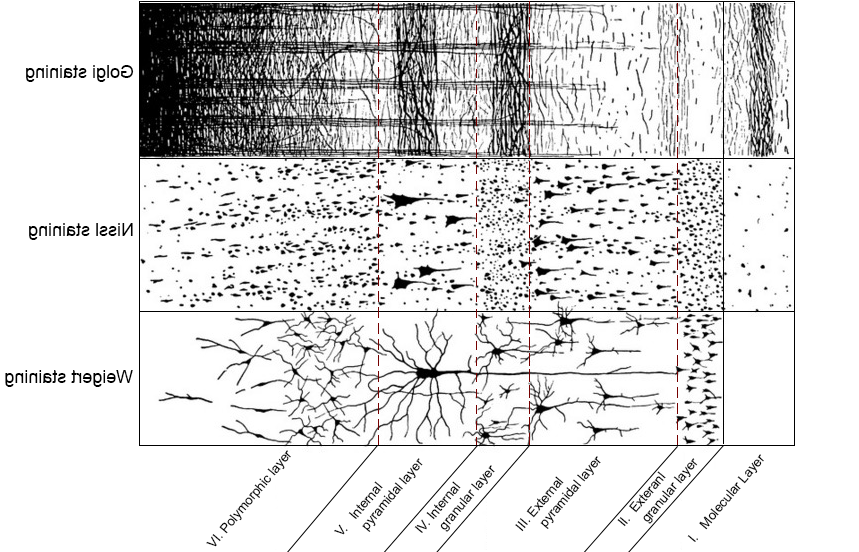
\includegraphics[width=0.8\textwidth, clip=true]{./Chapters/01_Introduction/Images/Layers}
	\caption{\cite{Brodman1909} }
	\label{fig:layers}
\end{figure}

For a small set of experiments, it is relatively straightforward to say if they are feed forward or feedback, but now think of more complicated processes: what would constitute as feed forward in language processing, decision making or memory? This is largely unknown and that is why it is of great interest to learn more about the laminar processing. It could shed light on a multitude of cognitive processes and open doors to a whole new type of information and new research in the brain \cite{Lawrence2017}. However, the greatest barrier is that is neuronal communication is not easily measured. With fMRI, only a derivative of neuronal firing can be measured as changes in oxygen consumption. We will therefore first need to get a better understanding of what type of information it is that fMRI can yield.

\section{Contrast Mechanisms}
Neurons clearly have layer specific functions, but measuring them is not easy, especially not in living humans. We cannot put electrodes in their heads, but what we can do is put them in an MRI scanner. An MRI scanner, however, cannot measure direct neuronal firing. Instead, it is susceptible to all kinds of magnetic properties of which three dimensional images can be made. Most notably, the magnetic susceptibility of red blood cells changes when they are oxygen rich or oxygen poor \cite{Ogawa1990}, which we call the Blood Oxygenation Level Dependant Signal, the BOLD signal. However, while there is little doubt that activation in a cortical region elicits a BOLD response, large parts of the biological mechanism behind it are still disputed. Most importantly, the extent to which the BOLD response reflects laminar specific activation is largely unknown. 

It was noted that maybe more so than just activity (MUA, multi unit acitvity), the amount of synaptic input (measured by the local field potential, LFP) migth be crucial for the strength of the BOLD response \cite{Goense2008}.

\begin{figure}[!ht]
	\centering
	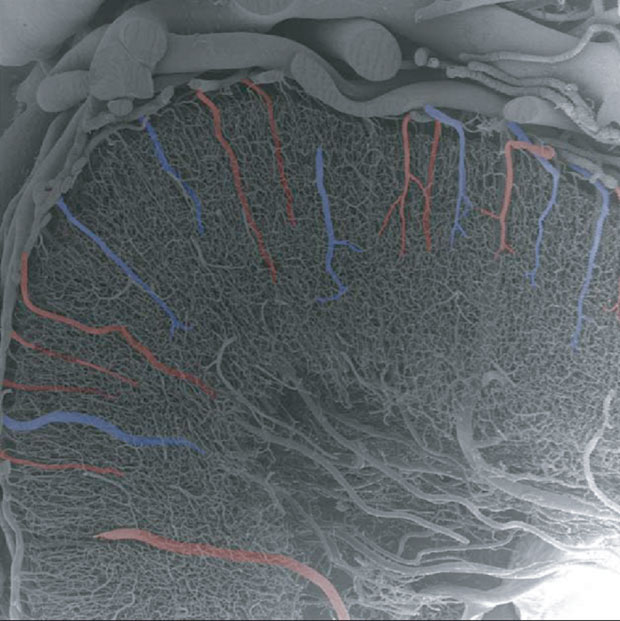
\includegraphics[width=0.9\textwidth, clip=true]{./Chapters/01_Introduction/Images/Microvasculature}
	\caption{The microvasculature of the visual cortex of a macaque \cite{Weber2008}. }
	\label{fig:microvasulature}
\end{figure}
Figure~\ref{fig:microvasulature} shows the microvasculature of a small piece of visual cortex in a macaque. In red, the arterioles, small blood vessels that dive from the top of the cortex (the pial surface) downward to supply the whole grey matter from blood. The smallest vessels, the capillaries, relay the oxygen to the neurons in all cortical layers, such that deoxygenated hemoglobin is drained away by the veins (blue). The veins on top of the cortex can be an order of magnitude larger than the cortical veins, and conduct off the deoxygenated blood. This might make one appreciate the difficulty of extracting laminar specific signals with large signals of non-interest in the direct neighbourhood. 

But the level of blood oxygenation is not the only quantity that fluctuates as a result of cortical activation. More blood starts flowing (higher cerebral blood flow, CBF), vessels start dilating (more cerebral blood volume, CBV) and the consumption of oxygen increases (higher cerebral metabolic rate of oxygen, CMR$_{O2}$). These quantitative measures can be related to one another by the Davis model, save some free parameters that need to be empirically determined \cite{Davis1997}. However, the proposed equations hold for the cortical column in its entirety, but does not take into account potential layer specific differences. 

So while we cannot measure neuronal activation with MRI, the closest we can get is the traces in the magnetic properties in the vasculature through BOLD, CBV, CBF, and CMRO$_{2}$. The extent to which these quantities vary as spatially specific as the level of the cortical layers is an outstanding question, however, and needs to empiraclly tested. Indeed, there are techniques to measure them, $T_2^*$-weighted imaging \cite{Norris2006} for BOLD, VASO for CBV \cite{Huber2018}, arterial spin labelling \cite{Grade2015} for CBV, and calibrated BOLD \cite{Blockley2013}) for CMRO$_{2}$. All vary in terms of sensitivity, specificity, and attainable resolution (spatial as well as temporal). The spatial resolution in combination with the type of experiment that is required for CBF and CMRO$_2$ measurements makes them poor candidates for human in vivo fMRI. It is mainly BOLD and CBV that have shown promising layer specific differences in animal experiments \cite{Lu2004,Zhao2006,Jin2008,Goense2012}. The main benefits of VASO compared to BOLD are its quantifiability \cite{Lu2003} and local specificity \cite{Jin2006}, whereas BOLD has higher sensitivity and speed \cite{Huber2018}.

Our main goal was to investigate the possibilities of laminar analysis in standard experiments on humans, and hence chose to use the BOLD signal as our signal of interest. Fundamentally, the BOLD signal arises as a consequence of magnetic field perturbations arising from desoxyhemoglobin molecules \cite{Norris2006}. These changes extend beyond the blood vessel and drop off as a function of field strength, the orientation of the vessel, and the vessel diameter. 
From the time that the molecules are excited until the time of the echo, molecules move around through the vessel. If the trajectory of a molecule in this time is small compared to the vessel size (and hence compared to the drop-off), there is little change in its surrounding magnetic field and the effect is reversible, a static effect. If on the other hand the molecule's trajectory is large, its surrounding magnetic field changes more drastically and unpredictably, such that the effect is irreversible and dynamic.
These two contrast mechanisms are the static and dynamic extravascular effect
The magnetic field perturbations scale linearly with field strength, so the trajectory of a molecule relative to the perturbations is much greater at 7 Tesla than at 1.5 Tesla. Thus, the dynamic extravascular effect increase with field strength. 
The remaining static effect at 7 Tesla is thus very specific, but detecting it requires high sensitivity \cite{Panchuelo2014}. 
An additional source of BOLD contrast is the intravascular effect. The magnetic field inside the vessel is slightly different from the surrounding tissue because of the amount of desoxyhemoglobin. As a result, the signal will start to dephase with respect to the extravascular signal. This is can be reversed because it is constant over time and is called the static intravascular effect. The exact origin of the last contrast mechanism is unclear. This is irreversible (dynamic) intravascular dephasing and has to do with the random movement of water molecules within red blood cells. It is either due to these water molecules interacting with the deoxyhemoglobin, or with the diffusion in and out of the cells, but no experiment to date has been able to tease the two mechanisms apart.
Four different contrast mechanisms can be distinguished.

Even given these four contrast mechanisms, it is still an outstanding question in what proportions they proliferate in measurements. This may even vary at the laminar level, as the deoxyhemoglobin from deeper layers flows upward to the top layers. The strengths of these effects have been modelled \cite{Markuerkiaga2016,Uludag2017} for both spin echo and gradient echo and suggest that most of the signal produced in a layer is also visible in that layer. For spin echo this is almost fully the case, while gradient echo has a tail that extents to more superficial layers, but at a gain of sensitivity. A range of laminar profiles has been found using spin echo (e.g. \cite{Zhao2004,Harel2006,Goense2006}), gradient echo (e.g. \cite{Polimeni2010,DeMartino2013,Chen2013}) or a combination of both, GRadient A Spin Echo (GRASE) \cite{Olman2012,DeMartino2013}.

Choosing a sequence requires carefully balancing the advantages and disadvantages against each other. We here chose to use gradient echo to investigate the laminar BOLD signal for its higher sensitivity at a field strength of 7 Tesla for high specificity. The potential downside of this is the susceptibility to the larger veins on top of the cortex that might obscure smaller effects \cite{Barth2007}. While the exact origins of the BOLD signal are unknown, there is strong evidence that the BOLD signal has a laminar footprint \cite{Logothetis2001}. Although some results from animal studies suggest that the effects may be visible at a higher temporal resolution than human in vivo MRI can achieve \cite{Yu2014,OHerron2016}. With the many uncertainties and the small size of the potential effect, it is soon clear that any potential effect can only be picked up with powerful methods that address as many sources of noise as possible. 

\subsection{Methods}
After covering the fundamentals of measurement techniques, it is clear what types of information may be expected to be present in the data. Getting out the relevant information, however, is at least as complicated. The brain is a highly convoluted structure that we are trying to describe and visualise by means of cubic voxel rasters. The first problem we encounter is a geometrical one: how do we attach a brain location to voxels in space? This can be done by making a \emph{cortical reconstruction} on a high resolution brain scan \cite{Dale1999,Bazin2012} with a very clear contrast between the white matter and grey matter as seen in Figure~\ref{fig:mybrain}. The distinction between white and grey matter is clear enough to draw a three dimensional boundary on both side of the grey matter: on the white matter boundary and one on the pial surface, the separation between the grey matter and the cerebrospinal fluid (CSF).
\begin{figure}[!ht]
	\centering
	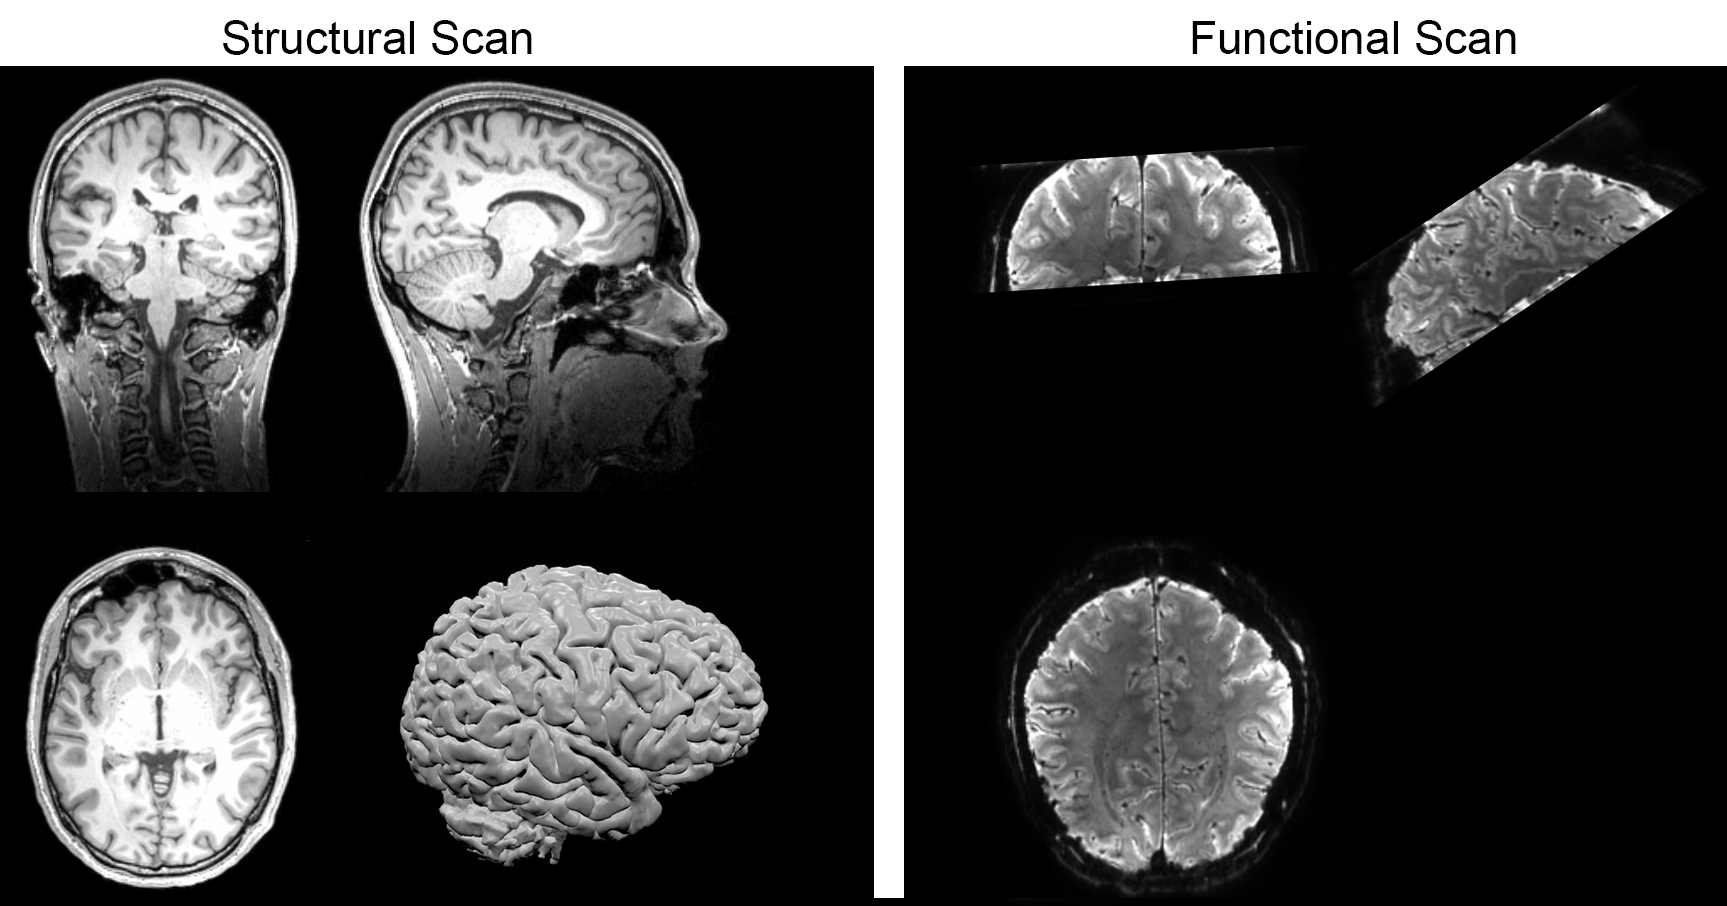
\includegraphics[width=0.99\textwidth, clip=true]{./Chapters/01_Introduction/Images/MyBrain}
	\caption{An example of a structural and functional brain scan. On the left, the structural scan has high anatomical contrast and sharp differences between the white matter and grey matter. The contrast is sharp enough to make a three dimensional reconstruction of the brain (lower right corner). On the right, a functional image is shown. The anatomical contrast is much weaker, but it can be acquired quickly and the contrast is susceptible to slight changes in blood deoxyhemoglobin, related to oxygen consumption on neuronal activation.}
	\label{fig:mybrain}
\end{figure}

The cortical reconstruction is very informative about the shape of the brain and potentially also about the layers: One could imagine different layers to be described as intermediate surfaces between both outer boundaries of which the locations can be used to then sample the cortical layers \cite{Koopmans2011,Polimeni2010,DeMartino2013}.
This descriptions allows for all sorts of surface base calculations \cite{Fischl2000,Bazin2012} and for example allows us to take into account a more naturalistic flow of the cortical layers \cite{Bok1929,Waehnertr2014}. Here it is described 



The people that we scan will move, breathe, fall asleep, ca
The scanner 


When we talk about a scanner with a field strength of 7 Tesla, it means there should be a homogeneous static magnetic field of that strength in the centre of the scanner. However, because the presence of a human body perturbs the field, it is not as homogeneous as one might want. Small perturbations can be corrected by \emph{shimming}, applying an additional magnetic field to compensate for the inhomogeneities. However, this is not accurate enough to correct all deviations and the inhomogeneities need not be constant over time. 


Distortion. The magnetic field is not always homogeneous



Multiple types 


It is possible geometrical properties 


%%
Balloon model \cite{Buxton1998}
something with a dynamic model of the hemodynamic signal \cite{Friston2000}.
















\section*{Thesis outline}
This thesis covers two major problems in laminar fMRI that needed to be solved before an experimental study could be conducted, and will reflect on building an fMRI pipeline, laminar or otherwise. In Chapter~\ref{ch:registration}, we will discuss a new way of coregistering an anatomical scan with a functional scan, when the latter is non-linearly distorted. We explain the details of the distortion correction technique, show its performance, and freely provide the code and data online. Chapter~\ref{ch:glm} describes a novel way of extracting laminar signal from data. We show its performance on a multitude of data, from a simulated fMRI model to post mortem data, to in vivo data from a set of subjects. Having overcome several of the most challenging aspects of laminar analysis, we then proceed to a laminar experiment in Chapter~\ref{ch:attention}. In a visual attention experiment, we investigate the laminar response. We further developped a new tool to more easily build fMRI analysis pipeline, to more reprodicibly conduct science, and to easily share analysis pipelines with others in Chapter~\ref{ch:porcupine}. Finally, these results will be put in a broader perspective in the Discussion, Chapter~\ref{ch:discussion}.


\linespread{1.5}
\newpage

%\linenumbers
\afterpage{\blankpage}
\chapter{Preserved Spontaneous Mentalizing amid Reduced Intersubject Variability in Autism during a Movie Narrative}
\label{ch:mentalizing_asc}

\begin{center}
    \large\textit{Abstract}
\end{center} 

{\abstractfont 
While individuals with autism often face challenges in everyday social interactions, they may demonstrate proficiency in structured mentalizing tasks that assess their ability to infer others' mental states. Using functional MRI and pupillometry, we investigated whether these discrepancies stem from diminished spontaneous mentalizing or broader difficulties in unstructured contexts. Fifty-two adults diagnosed with autism and 52 neurotypical controls viewed 'Partly Cloudy', a nonverbal animated film with a dynamic social narrative known to engage the mentalizing brain network during specific scenes. Analysis focused on comparing brain and pupil responses to these mentalizing events. Additionally, dynamic intersubject correlations explored the variability of these responses throughout the film. Both groups showed similar brain and pupil responses to mentalizing events and provided comparable descriptions of the characters' mental states. However, participants with autism exhibited significantly stronger correlations in their responses across the film's social narrative, indicating reduced inter-individual variability. This distinct pattern emerged well before any mentalizing events and involved brain regions beyond the mentalizing network. Our findings provide functional evidence of spontaneous mentalizing in autism, demonstrating this capacity in a context affording but not requiring mentalizing. Rather than responses to mentalizing events, a novel neurocognitive signature - inter-individual variability in brain and pupil responses to evolving social narratives - differentiated neurotypical individuals from those with autism. These results suggest that idiosyncratic narrative processing in unstructured settings, a common element of everyday social interactions, may offer a more sensitive scenario for understanding the autistic mind. \par
} 

\vspace*{\fill} 
This chapter is adapted from: \bibentry{mangnus2024bpcnni}

\thispagestyle{empty}

\newpage

\section{Introduction}
Autism Spectrum Condition (ASC) is a neurodevelopmental disorder marked by difficulties in social communication and interaction across multiple contexts \citep{apa2013}. These difficulties are frequently associated with mentalizing - the ability to attribute mental states to oneself and others \citep{premack1978,wimmer1983}. While initial findings suggested diminished mentalizing abilities in autism \citep{baron-cohen1985,happe1994}, subsequent studies have painted a more complex picture, owing to a variety of factors.

First, the reliability of established mentalizing assessments, such as the False Belief Test, Strange Stories, and the Reading the Mind in the Eyes Test, has increasingly come under scrutiny. These tests have shown inconsistent effect sizes when compared to earlier, smaller-scale studies and exhibit limited correlations with one another, despite their aim to measure similar or identical mentalizing constructs \citep{gernsbacher2019,higgins2024,schaafsma2015,yeung2024}. Second, many studies do not adequately match autistic individuals with neurotypical controls based on language abilities, which are crucial to varying degrees for these tasks \citep{betz2019}. This lack in language matching is particularly significant given the generally lower performance in verbal learning and memory observed within the autism population \citep{velikonja2019}. Lastly, recent research highlights the remarkable proficiency of autistic individuals in mentalizing tasks, especially in situations requiring strategic mental state reasoning \citep{bowler1992,pantelis2017}, such as deception \citep{vantiel2021}.

Faced with these empirical challenges, researchers have turned to more implicit mentalizing measures. This includes the analysis of anticipatory eye movements concerning an actor's false beliefs \citep{senju2009}, and measuring neural activity in the Animated Triangles task, where participants attribute mental states to moving shapes \citep{abell2000}. Recent findings indicate that while autistic individuals do show anticipatory gaze responses, these responses tend to be generally slower, regardless of whether the character's beliefs were true or false \citep{glenwright2021,schuwerk2016}. In the Animated Triangles task, both autistic and neurotypical participants show comparable brain activation in key mentalizing regions, such as the medial prefrontal cortex (mPFC), temporoparietal junction (TPJ), and precuneus \citep{moessnang2020}. However, individuals with autism typically underperform in both the mentalizing and non-mentalizing conditions of this task, which, combined with their generally slower anticipatory gaze responses, points to broader difficulties in implicit task settings \citep{wilson2021}. The extent to which autistic individuals engage in spontaneous mentalizing, particularly in unstructured settings lacking an explicitly defined task, as is common in everyday social interactions, remains largely unknown.

In this study combining fMRI and pupillometry, we aimed to bridge this knowledge gap by investigating how individuals with and without autism respond to mental state events embedded in a dynamic movie narrative. Additionally, we sought to provide insights into how these individuals process stimuli in less structured environments that more closely resemble everyday social interactions. Everyday interactions require a continuous assessment of stimuli within an evolving narrative \citep{goffman1974,johnson2023,stolk2022}, as seen in how even seemingly minor behaviors like a voluntary cough or a brief silence can carry significant implications in certain contexts \citep{kendon1994}. Failure to recognize these narrative cues could lead to misunderstandings in scenarios that require high levels of interpretation, such as irony or sarcasm, areas known to pose challenges for autistic individuals \citep{deliens2018,zalla2014}. However, capturing this narrative processing is challenging, as it likely unfolds differently over time among individuals exposed to the same stimuli. We reasoned that narrative processing could manifest as inter-individual variability in responses to movie stimuli, particularly diminished among those less inclined to interpret stimuli through a narrative lens \citep{chang2021,finn2018,owen2023,zhang2022}. We investigated this possibility using intersubject correlation analysis \citep{hasson2004}, applying it to two complementary methods for assessing cognitive processing: brain imaging and measurements of pupil size \citep{beatty1982}. 

To probe spontaneous mentalizing and narrative processing, we recorded participants' brain and pupil responses as they viewed the nonverbal animated movie `Partly Cloudy'\citep{jacoby2016,paunov2019}. Although movies cannot fully replicate the complexities of real-world social interactions \citep{wheatley2019}, they offer an effective platform for immersing participants in an evolving narrative under uniform stimulus conditions. To assess differences in narrative processing between autistic and neurotypical participants at various points during the movie, we augmented our intersubject correlation analysis with a dynamic sliding window technique and an adaptive clustering algorithm \citep{maris2007}. The movie Partly Cloudy was chosen for its proven ability to evoke neural activations within the mentalizing network through distinct mental state events \citep{jacoby2016,richardson2018}, making it suitable for evaluating spontaneous mentalizing. After viewing, we analyzed participants' verbal descriptions of the movie, focusing on their use of language related to mental states. This experimental approach enabled us to simultaneously probe spontaneous mentalizing and narrative processing, providing insights into how these cognitive functions interact in individuals with autism.

\section{Materials and methods}
\subsection{Preregistration and Data availability}
The study comprised two sets of preregistered analyses \citep{mangnus2022}. The first set focused on spontaneous pupil and brain responses to movie events anticipated to elicit mental state inferences, complemented by a questionnaire that examined participants' use of related vocabulary in describing the movie. The second set of analyses explored dynamic intersubject correlations to investigate idiosyncratic narrative processing throughout the entire movie. Unlike the event-related analyses, these exploratory analyses were not limited to specific movie segments. All resulting pupillometry and fMRI data are publicly available for further research \citep{mangnus2024dataset}. 

\subsection{Participants} 
The study enrolled 104 participants, divided equally into 52 adults diagnosed with Autism Spectrum Disorder (ASC) and 52 neurotypical controls (NT). Recruitment occurred through Radboud University's database, social media, campus postings, and outpatient clinics in Nijmegen and Arnhem, the Netherlands. Eligibility for the ASC group required a formal diagnosis from a clinician \citep{apa2013}, while exclusion criteria for all included the use of psychotropic drugs, severe cognitive impairment, systemic diseases, or neurological treatment history. As shown in Table~\ref{tab:ppt-stats-asc}, both groups were demographically matched for gender, age (Kullback-Leibler divergence = .05, \textit{F}-test (102) = .29), and both verbal and nonverbal IQ, verified through the Similarities and Vocabulary subscales of the Wechsler Adult Intelligence Scale (WAIS-III \citep{wechsler1997}; KL = .02, \textit{F}-test = .74) and Raven's Progressive Matrices (RPM \citep{raven1989}; KL = .01, \textit{F}-test (102) = .63). ASC participants notably scored higher on the Autism-Spectrum Quotient (AQ-50 \citep{baron-cohen2001AQ}), confirming group distinctions. Data collection involved MRI scans (\textit{n} = 104) and pupillometry (\textit{n} = 100) while participants viewed the film, followed by a post-viewing questionnaire completed by most (\textit{n} = 101). All participants provided written informed consent, approved by the local ethics committee (CMO region Arnhem-Nijmegen, file number 2019-6059), and received compensation for participation.

\begin{table}[ht]
    \captionsetup{justification=raggedright, singlelinecheck=false, font = normal} % Left-align the caption
    \caption{Demographic data}
    \label{tab:ppt-stats-asc}
    \setlength{\tabcolsep}{10pt}
    \renewcommand{\arraystretch}{1.5} % Adjust row spacing (default is 1.0)
    \begin{tabular}{llll}
    \hline
    \textbf{} & \textit{ASC Group} & \textit{NT Group} & \textit{Group Difference} \\
    \hline
    N (men:women) & 52 (23:29) & 52 (20:32) & \textit{$\chi$\textsuperscript{2}}(1, \textit{N} = 104) = 1.73, \textit{p} = .19 \\
    Age (years) & 27.7 (6.3) & 25.9 (5.5) & \textit{t}(102) = 1.74, \textit{p} = .08 \\
    Verbal IQ (WAIS-III) & 126 (16) & 124 (16) & \textit{t}(102) = 0.51, \textit{p} = .61 \\
    Nonverbal IQ (RPM) & 103 (9) & 104 (11) & \textit{t}(102) = -0.46, \textit{p} = .64 \\
    Autism Quotient & 31 (9) & 12 (6) & \textit{t}(102) = 12.2, \textit{p} < .001 \\
    \hline
    \multicolumn{4}{l}{\small{Values are given as Mean (Standard Deviation). ASC, Autism Spectrum Condition; NT, Neurotypical.}} \\
    \end{tabular}
\end{table}
    

\subsection{Experimental design }
Participants watched the 5-minute and 45-second animated short Partly Cloudy, depicting the evolving friendship between a stork and a cloud through various social interactions integral to its narrative. After viewing, they described the plot to assess narrative comprehension and articulation of characters' mental states. Descriptions were analyzed by independent raters, categorizing words into mental state terms or other content-related categories, using the mental state word list from \cite{bang2013}. An independent \textit{t}-test compared the frequency of mental state words used between groups. The movie featured three types of events, coded by the original research team that introduced it as a mentalizing localizer task \citep{jacoby2016}. These included \textit{Mental}, \textit{Pain}, and \textit{Control} events, each annotated on the movie's timeline in Fig~\ref{fig:task-fig-asc}. \textit{Mental} events, totaling 44 seconds across 4 events, were expected to elicit inferences about characters' mental states, depicting scenarios like characters feeling distressed while observing others enjoy a cheerful interaction or mistakenly perceiving betrayal by a friend. \textit{Pain} events, totaling 26 seconds across 7 events, depicted instances where characters experienced physical discomfort, such as being shocked by an eel or bitten by a crocodile. \textit{Control} events, totaling 24 seconds across 3 events, showcased serene moments like birds in flights or panoramic views of clouds. As detailed in later sections, these categorizations facilitated the analysis of mentalizing-related pupillary and neural responses.

\begin{figure}[!ht]
	\centering
    \makebox[\textwidth][c]{\includegraphics[width=1.05\textwidth]{./Chapters/02_MentalizingASC/Images/TaskFig.eps}}
	\caption{Autistic and neurotypical participants viewed a six-minute animated movie portraying the evolving friendship between a stork and a cloud, while their pupil and brain responses were recorded. Originally used by Jacoby et al. (2016) as a Theory of Mind localizer, the movie includes three types of events: Mental, Pain and Control, each marked on the movie timeline. Mental and Pain events were expected to prompt inferences about characters' mental and physical states, whereas Control events featured no characters in the foreground. The event images shown were generated using Copilot in Bing for copyright purposes to closely resemble scenes from the movie.}
    \vspace*{-10pt}
	\label{fig:task-fig}
\end{figure}

%[width=.9\textwidth]



\subsection{Pupillometry and MRI data acquisition}
Pupil size was continuously tracked using an Eyelink 1000 plus eyetracker at 1000 Hz. MRI data were acquired using a Siemens 3T MRI-scanner with a 32-channel head coil. Structural images were obtained with a T1 MPRAGE sequence (TR = 2200 ms, TI = 1100 ms, TE = 2.6 ms, flip angle = 11\textdegree, 
voxel size = 0.8 mm\textsuperscript{3}, acceleration factor = 2). Functional images were acquired with a multi-band multi-echo sequence (TR = 1500 ms, TE = 13.4/34.8/56.2 ms, flip angle = 75\textdegree, voxel size = 2.5 mm\textsuperscript{3}, acceleration factor = 2). Analysis of head movement through framewise displacement (FD) showed no significant differences between the ASC and NT groups. Mean FD was 0.15 \textpm{}{} 0.05 for ASC and 0.16 \textpm{}{} 0.09 for NT (M \textpm{} SD; \textit{t}(102) = -0.78, \textit{p} = .43), with maximum FD values at 0.81 \textpm{} 0.79 for ASC and 1.03 \textpm{} 1.31 for NT (\textit{t}(102) = -1.09, \textit{p} = .28). Additionally, assessments of total head motion, calculated from translation and rotation during the realignment process, indicated no significant differences (Translation: 109.5 \textpm{} 74.6 vs. 114.3 \textpm{} 99.5, \textit{t}(102) = 0.28, \textit{p} = .78; Rotation: 2.0 \textpm{} 0.98 vs. 2.2 \textpm{} 1.2 , \textit{t}(102) = 0.74, \textit{p} = .46).

\subsection{Pupillometry data analysis}
Pupillometry data underwent preprocessing with a combination of established and custom MATLAB routines. Blinks were removed using a noise-based detection algorithm \citep{hershman2018}. Squints, marked by unusually small pupil sizes \citep{mathot2018}, and gaze jumps, indicative of excessive translational eye movements, were both identified and eliminated through visual inspection. After these adjustments, 89.3\% \textpm{} 9.4\% of the data remained usable for the ASC group and 88.4\% \textpm{} 10.6\% for the NT group (\textit{t}(98) = 0.48, \textit{p} = .63). Fixations and saccades were distinguished using an adaptive velocity threshold \citep{nystrom2010}. Pupil timeseries were normalized (\textit{z}-scored) and adjusted for global luminance fluctuations modeled using the \textit{lm()} function from the R \textit{stats} package \citep{bates2015} up to the 5th polynomial order, validated with data from five randomly selected participants. Luminance was quantified using RGB values based on the Rec. 709 formula \citep{itu2002}. 

Event-related pupil responses were analyzed through a 3x2 mixed-design ANOVA with mean pupil size as the dependent variable, and event conditions (\textit{Mental, Pain, Control}) and participant group status (ASC, NT) as factors. Tukey's Honest Significant Difference tests further investigated mentalizing-related contrasts, specifically comparing \textit{Mental} to both \textit{Pain} and \textit{Control} conditions. To verify the robustness of our findings against variations in event timing, a control analysis was conducted by incorporating an additional time-based regressor into the \textit{lm()} function during preprocessing. This adjustment, which incremented by one every second, did not influence the main findings.

Intersubject variability was assessed using dynamic intersubject correlation analysis of the pupil timeseries. Employing a leave-one-out approach, each participant's timeseries was correlated with the composite average timeseries of all other group members \citep{nastase2019}. This analysis was conducted using a 30-second sliding window at 100 ms intervals, generating a correlation timeseries for the entire movie duration per participant. All correlation timeseries were Fisher \textit{z}-transformed and subjected to a nonparametric cluster-based permutation test \citep{maris2007}. This test addresses the multiple comparisons problem in timeseries analysis by clustering significant neighboring data points. These clusters are tested against a null distribution formed by randomly shuffling participant labels and recalculating statistics, allowing the identification of specific timepoints where significant differences in pupil response variability between groups occurred, while effectively controlling for false positives. Statistical testing was performed using a two-sided independent samples \textit{t}-test with 10,000 permutations to establish the null distribution. Clusters that reached a Monte-Carlo \textit{p}-value of .05 or less were considered statistically significant.

\subsection{fMRI data analysis}
Functional images were preprocessed using SPM12, initially consolidating multiple echoes into single volumes through echo-weighted combinations. These volumes were realigned to the initial image using rigid-body transformations and 2nd degree B-spline interpolation, and subsequently unwarped with participant-specific fieldmaps to minimize spatial distortions and signal dropout. Anatomical images were coregistered to the mean functional image and segmented into gray matter, white matter, and cerebral spinal fluid categories using SPM's tissue probability maps, enabling normalization to MNI space. An 8 mm full-width at half-maximum kernel was applied or spatial smoothing. First-level regressors estimated activations for \textit{Mental, Pain,} and \textit{Control} events, and included adjustments for head movement (using squared and cubic terms, along with first and second derivatives) and tissue signal intensities. A 0.6 threshold masking was applied to ensure optimal brain coverage.

Two 2-by-2 mixed-design ANOVAs were conducted to analyze mentalizing activations across \textit{Mental, Pain,} and \textit{Control} conditions and participant groups (ASC, NT). The first contrast (\textit{Mental} > \textit{Pain}) sought to confirm previous findings of enhanced mentalizing network activity \citep{jacoby2016}, while the second (\textit{Mental} > \textit{Control}) extended these findings to scenes lacking foreground characters. Results were subjected to whole-brain, cluster-level correction (\textit{p\textsubscript{FWE}} < .05), with anatomical locations identified using the SPM Anatomy Toolbox \citep{eickhoff2005}. Additionally, a region of interest (ROI) analysis focused on three peak brain regions, complemented by Bayesian analysis \citep{jasp2022} to evaluate consistent neural activation within the mentalizing network across groups, reporting evidence with Bayes Factors (BFs). Robustness against event timing variations was confirmed through a control analysis adding a first-level regressor that incremented with each volume.

Intersubject variability at the neural level was assessed using dynamic intersubject correlation analysis of voxel timeseries, adjusted for head movement and tissue signals. Mirroring the pupillometry analysis, a leave-one-out and sliding window method generated whole-brain correlation timeseries for each participant. For computational efficiency, the data were spatially and temporally downsampled by a factor of three, resulting in a voxel resolution of 7.5 mm and a sampling interval of 4.5 seconds. These data underwent a nonparametric cluster-based permutation test \citep{maris2007}, which corrected for multiple comparisons across voxels and timepoints using a two-sided independent samples \textit{t}-test with 10,000 permutations (Monte-Carlo \textit{p} < .05). The analysis was further refined with a spatially adaptive clustering algorithm, identifying variations in brain response patterns between groups. The spatial distribution of the identified spatiotemporal brain cluster was visualized by summing t-values across all timepoints, producing a three-dimensional representation of significant variability. The degree of overlap between this cluster and the mentalizing network was quantified by comparing their spatial volumes. Lastly, a supplementary analysis without the sliding window approach calculated correlations across the entire voxel timeseries, pinpointing a smaller cluster in the left supramarginal gyrus. In line with the main findings, this cluster demonstrated reduced intersubject variability in the ASC group.

\section{Results}
\subsection{Post-viewing movie descriptions }
After the film viewing, participants were asked to recount the story of the stork and cloud's evolving friendship in their own words. We analyzed these descriptions for the use of mental state words and other content-related terms (Fig~\ref{fig:beh-pupil-asc}a). Statistical analysis revealed no significant differences in the frequency of mental state word usage between the autistic and neurotypical participants (M\textsubscript{ASC} = 0.063, M\textsubscript{NT} = 0.054, \textit{t}(99) = 0.84, \textit{p} = .40; Fig. 2b), with a Bayes Factor in favor of the null hypothesis (BF\textsubscript{Null} = 3.49). This finding suggests that both autistic and neurotypical groups engaged similarly with the mental states depicted in the film.

\begin{figure}[!ht]
    \vspace*{10pt}
	\centering
    \makebox[\textwidth][c]{\includegraphics[width=1.05\textwidth]{./Chapters/02_MentalizingASC/Images/BehPupil.eps}}
	\caption{Comparable mental state descriptions and pupil responses across groups. (a) Word Cloud depicting the frequency of mental state-related vocabulary used by participants in their post-viewing movie descriptions. The size of each word corresponds to its frequency of use. (b) Bar graphs displaying the ratio of mental state words to other content-related terms in these descriptions, showing no significant differences between the two groups. (c) Pupil responses across all event conditions, revealing similar response patterns in both autistic and neurotypical groups. Asterisks denote significant differences between event conditions (all \textit{p} < .001), with no significant differences observed between groups. Outliers are represented by dots, while whiskers display a 1.5 inter-quartile range.}
    \vspace*{-10pt}
	\label{fig:beh-pupil-asc}
\end{figure}



\subsection{Event-related pupil responses}
Participants' pupil sizes were continuously tracked throughout the movie to assess responses to events expected to elicit mental state inferences, such as the cloud reflecting on the stork's actions. We also analyzed responses to events evoking physical state inferences, like the stork experiencing pain, as well as to control scenes devoid of character interactions. Pupillometry analysis identified distinct responses to these three event types (\textit{F}(2,196) = 73.0, \textit{p} < .001, BF\textsubscript{Null} = 0.00; Fig~\ref{fig:beh-pupil-asc}c), with the largest pupil dilation occurring during \textit{Pain} events (M = 0.22, \textit{z}-score), followed by \textit{Mental} events (M = -0.12) and \textit{Control} events (M = -0.20). Comparisons of pupil responses between autistic and neurotypical participants revealed no significant differences (\textit{F}(1,98) = 0.03, \textit{p} = .86, BF\textsubscript{Null} = 7.8), nor were there significant interaction effects between participant groups and event types (\textit{F}(2,196) = 2.1, \textit{p} = .12, BF\textsubscript{Null} = 2.5). This suggests that both groups reacted similarly to the different event types in the movie.

\subsection{Event-related brain responses}
A whole-brain fMRI analysis was conducted to examine neural activations during \textit{Mental} events in comparison to \textit{Control} and \textit{Pain} events. As depicted in Fig~\ref{fig:fmri-results-asc}a, this analysis identified robust activation in keys areas of the mentalizing network \citep{schurz2014}, specifically in the right and left temporoparietal junction (rTPJ: xyz\textsubscript{MNI} = [48, -62, 32], \textit{t} = 16.85, \textit{p\textsubscript{FWE}} < 0.001; lTPJ: [-46, -62, 32], \textit{t} = 16.92, \textit{p\textsubscript{FWE}} < 0.001), the precuneus ([6, -64, 40], \textit{t} = 20.64, \textit{p\textsubscript{FWE}} < 0.001), medial prefrontal cortex (mPFC: [-6, 52, 38], \textit{t} = 7.33, \textit{p\textsubscript{FWE}} < 0.001), and left middle temporal gyrus ([-52, 2, -26], \textit{t} = 11.51, \textit{p\textsubscript{FWE}} < 0.001). Echoing the pupillometry findings, no significant differences in neural activation were observed between autistic and neurotypical participants. Complementary region of interest (ROI) analyses (Fig~\ref{fig:fmri-results-asc}b) and Bayesian analyses reinforced these findings, providing evidence favoring the null hypothesis over alternative models suggesting group differences. This was consistently demonstrated across all evaluated ROIs for both \textit{Mental} > \textit{Pain} contrasts (rTPJ: BF\textsubscript{Null} = 4.83, precuneus: BF\textsubscript{Null} = 1.73, mPFC: BF\textsubscript{Null} = 4.01) and \textit{Mental} > \textit{Control} contrasts (rTPJ: BF\textsubscript{Null} = 3.43, precuneus: BF\textsubscript{Null} = 3.63,  mPFC: BF\textsubscript{Null} = 4.71), underscoring a similarity in neural processing of mental states among autistic and neurotypical individuals.

\begin{figure}[!ht]
	\centering
    \includegraphics[width=1\textwidth,trim={0 9cm 0 0},clip=true]{./Chapters/02_MentalizingASC/Images/FMRIResults.eps}
	\caption{Comparable neural activation patterns during mental state events across groups. (a) Brain sections showing whole-brain responses specific to mental state events, as assessed through the Mental > Control and Mental > Pain contrasts. There were no significant differences in activation for either contrast between the autistic and neurotypical groups. (b) Box plots depicting the contrast estimates for the Mental > Control (in blue) and Mental > Pain (in red) comparisons across various Regions of Interest (ROI) for both groups. rTPJ and mPFC were selected as ROIs based on mentalizing literature, while the precuneus was selected because of the peak voxel being located in that region for both mentalizing contrasts. Across all ROIs and contrasts, no significant differences were observed between the groups. Outliers are represented by dots, while whiskers display a 1.5 inter-quartile range.}
    \vspace*{-10pt}
	\label{fig:fmri-results}
\end{figure}

%\makebox[\textwidth][c]{



\subsection{Movie-driven variability in pupil responses }
Having observed comparable pupil and brain responses to mental state events and similar verbal descriptions from both autistic and neurotypical participants, we expanded our investigation to narrative processing differences across the entire movie through dynamic intersubject correlation analysis of the pupil timeseries. This analysis revealed an interval from 40 to 71 seconds where individuals with autism demonstrated significantly stronger correlations in pupil responses, indicating reduced intersubject variability compared to neurotypical participants (M\textsubscript{ASC} = 0.61, M\textsubscript{NT} = 0.55, \textit{cluster stat} = 777, \textit{p} = .045; Fig~\ref{fig:isc-pupil-asc}). This interval preceded any mental state events and coincided with scenes featuring storks flying through the air and clouds morphing into baby animals. Although this reduced variability continued throughout the film, it did not reach statistical significance outside this interval after adjusting for multiple comparisons. Further, differences in variability were not due to variations in saccadic eye movements, as their frequency and variability remained consistent between groups (Fig~\ref{fig:saccades-suppl}).

\begin{figure}[!ht]
    \vspace*{5pt}
	\centering
    \includegraphics[width=1\textwidth,clip=true]{./Chapters/02_MentalizingASC/Images/ISCPupil.eps}
	\caption{Reduced pupil response variability in autistic participants. Dynamic intersubject correlation analysis initially showed comparably high levels of correlation in both autistic and neurotypical groups at the start of the movie. However, a significant divergence emerged around the 40-second mark, where autistic individuals showed stronger correlations in their pupil responses, indicating reduced intersubject variability, compared to neurotypical participants. This pattern of reduced variability emerged well before the mental state events highlighted in red. Solid lines delineate statistically significant intervals, as determined by a cluster-based permutation test.}
    \vspace*{-15pt}
	\label{fig:isc-pupil-asc}
\end{figure}





\subsection{Movie-driven variability in brain responses}
When applied to the fMRI data, dynamic intersubject correlation analysis identified a spatiotemporal cluster where individuals with autism showed significantly stronger correlations in their brain responses compared to neurotypical participants (Fig~\ref{fig:isc-fmri-time-asc}). This cluster spanned the entire movie (\textit{cluster stat} = 1332, \textit{p} = .002) and included peaks in the right and left supramarginal gyrus (rSMG: xyz\textsubscript{MNI} = [52, -34, 32], \textit{t\textsubscript{max}} = 3.88; lSMG: [-54, -40, 32], \textit{t\textsubscript{max}} = 4.54), the right inferior temporal gyrus (rITG: [54, -22, -28], \textit{t\textsubscript{max}} = 5.90), and the left calcarine gyrus (lCG: [6, -102, -10], \textit{t\textsubscript{max}} = 4.20). The reduced variability was consistent across these regions for most of the movie (Fig~\ref{fig:isc-fmri-peak-suppl}), and it emerged well before and continued after any mental state events. The cluster's overlap with the mentalizing network was minimal, comprising less than 20\% of the total cluster size (Fig~\ref{fig:isc-fmri-overlap-asc}). This indicates that the observed reduced variability in brain responses among autistic participants extends beyond regions involved in mental state processing, suggesting broader differences in neural processing between the groups.

\begin{figure}[!ht]
	\centering
    \makebox[\textwidth][c]{\includegraphics[width=1.05\textwidth,clip=true]{./Chapters/02_MentalizingASC/Images/ISCFMRITime.eps}}
	\caption{Reduced brain response variability in autistic participants. Dynamic intersubject correlation analysis identified a spatiotemporal brain cluster where autistic individuals demonstrated significantly stronger correlations in their brain responses, indicating reduced intersubject variability, compared to neurotypical participants. This cluster persisted throughout the movie and featured peaks in the right and left supramarginal gyrus, the right inferior temporal gyrus, and the left calcarine gyrus. Echoing the pupillometry data, this pattern of reduced variability in autistic participants emerged well before the mental state events highlighted in red. LH, left hemisphere; RH, right hemisphere.}
    \vspace*{-10pt}
	\label{fig:isc-fmri-time-asc}
\end{figure}





\vspace*{.1cm}

\begin{figure}[!ht]
	\centering
    \includegraphics[width=1\textwidth,clip=true]{./Chapters/02_MentalizingASC/Images/ISCFMRIOverlap.eps}
	\caption{Limited spatial overlap between brain regions showing reduced intersubject variability in autistic participants and mentalizing activation. The overlap comprised less than 20\% of the total cluster size. For clarity, the cluster is visualized using a cumulative \textit{t}-value threshold of 20 or higher. Lateral brain images provide an overlay with a search distance of 10 mm. }
    \vspace*{-10pt}
	\label{fig:isc-fmri-overlap}
\end{figure}





\section{Discussion}
Using fMRI and pupillometry, this study provides functional evidence of spontaneous mentalizing abilities in individuals with autism. Compared to neurotypical controls matched for gender, age, and both verbal and nonverbal IQ, individuals with autism exhibited similar brain and pupil responses during movie scenes known to activate the mentalizing network \citep{jacoby2016,richardson2018}. Activity in the mentalizing network was enhanced during scenes that encouraged viewers to contemplate the actions and mental states of depicted characters. Conversely, scenes prompting physical state inferences, such as characters experiencing physical discomfort, or control scenes lacking central characters, resulted in weaker mentalizing activations. Verbal descriptions provided by participants after the movie corroborated these findings, indicating an engagement with the mental state events depicted in the movie on par with that of neurotypical controls. These results extend prior evidence of preserved mentalizing in autism \citep{moessnang2020,dufour2013}, showcasing this capacity in a situation affording but not requiring mentalizing.

While individuals with and without ASC showed comparable brain and pupil responses during mental state events, dynamic intersubject correlation analysis revealed significant differences in the correlation of these responses over extended movie intervals. Participants with autism exhibited significantly stronger correlations, indicating reduced inter-individual variability, across several brain regions outside the mentalizing network. These regions included the right and left supramarginal gyrus, linked to empathic judgment \citep{silani2013,wada2021}, the right inferior temporal gyrus, associated with narrative comprehension \citep{youssofzadeh2022}, and the left calcarine gyrus, crucial for visual processing \citep{woldorff2002}. This reduced variability was not due to differences in bottom-up processing, as both autistic and neurotypical groups exhibited similar saccadic eye movement patterns throughout the film. The most pronounced differences emerged during early scenes featuring storks flying through the air and clouds morphing into baby animals, which likely introduced significant narrative ambiguity. This ambiguity may have prompted neurotypical viewers to idiosyncratically interpret how these visual elements fit into the evolving storyline, resulting in less consistent responses. In contrast, autistic participants' responses appeared to be more consistently aligned with the movie's stimuli, possibly reflecting a heightened focus on specific details rather than the broader narrative context \citep{losh2003,tager-flusberg1995,barnes2012,geelhand2020,koldewyn2014}. Importantly, these differences manifested in cognitive and neural processing rather than in eye movements, suggesting that the variability observed in neurotypical responses may represent a neurocognitive signature of top-down processing.

The neuroanatomical bases of the observed changes in response variability are in line with existing research on autism and social interaction. Prior studies have documented structural alterations in the gray matter of both the right and left supramarginal gyrus in individuals with autism \citep{brieber2007,ke2008,libero2014}, as well as reduced anatomical connectivity in the right inferior temporal cortex \citep{boets2018,koldewyn2014}. This region exhibits prolonged activations during tasks involving story comprehension and interactive communication \citep{youssofzadeh2022,stolk2013neural}, highlighting its role in integrating stimuli within an evolving narrative. This integration is crucial for complex social interactions, which necessitate the continuous assessment of diverse stimuli to maintain narrative coherence with others \citep{goffman1974,johnson2023,stolk2022}. A key direction for future research is to examine how response variability in the identified brain regions differs across various social contexts. Such investigations will not only help to illuminate the specific challenges faced by autistic individuals in everyday social situations, but could also inform the development of interventions by identifying environments that promote effective social interaction \citep{wadge2019}.

It is worth noting that our intersubject correlation patterns differ from previous studies demonstrating greater brain response variability in autistic individuals compared to neurotypicals \citep{byrge2015,hahamy2015,hasson2009,lyons2020,nunes2019,ou2022,pegado2020,salmi2013}. Several factors could explain these discrepancies. First, our study used an animated film with fictional characters, as opposed to the more realistic human portrayals in other studies. Although the type of characters may influence brain responses in autism \citep{atherton2018}, greater neural variability has been noted with fictional characters \citep{lyons2020}. Second, we implemented an adaptive clustering algorithm to identify spatiotemporal clusters of brain response variability within 30-second intervals. This approach is potentially more sensitive to brain response variations associated with subtle shifts in interpretation than whole-movie analyses, which emphasize consistent patterns over significantly longer durations (10 to 67 minutes). This approach may more effectively capture the hypothesized increased reliance on bottom-up sensory stimulation in autism \citep{pellicano2012}, possibly leading to less variability in neural signals related to narrative interpretation. More generally, our findings invite a reconsideration of theories that propose precise neural synchronization as a means to manage individual perspectives in daily interactions \citep{holroyd2022}. These theories suggest that aligning neural responses to external cues helps individuals achieve a common viewpoint, thereby facilitating social interaction \citep{hasson2012,mayo2021}. However, contrary to expectations based on their social difficulties, participants with autism in our study displayed stronger neural correlations when exposed to the same external stimuli, challenging the assumed role of precise neural synchronization in social interaction \citep{stolk2014}.

In conclusion, this study offers functional evidence of spontaneous mentalizing in autism, showcasing this capacity in a context affording but not requiring mental state inferences. More distinctively, our findings identify a novel neurocognitive signature - inter-individual variability in brain and pupil responses to evolving social narratives - that differentiates neurotypical individuals from those with autism. These results underscore the importance of idiosyncratic narrative processing in unstructured settings, a hallmark of everyday social interactions, as a potentially more sensitive framework for understanding the autistic mind.
\newpage  
\section{Supplementary information} 

% table S1. 
\begin{table}[ht]
    \centering
    \captionsetup{justification=raggedright, singlelinecheck=false, font = normal} % Left-align the caption
    \setlength{\tabcolsep}{6pt} % Adjust column spacing if needed
    \renewcommand{\arraystretch}{1.5} % Adjust row spacing
    \caption{Results of the within-subject fMRI analyses related to the main effects of event type (Mental, Pain, Control).}
    \label{tab:fmri_anova}
    \small
    \begin{tabular}{lllccccc}
    \hline
    \textit{Contrast} & \textit{Anatomical location of peak voxel} & \textit{Cluster size} & \multicolumn{3}{c}{\textit{MNI coordinates}} & \textit{T-value} \\
     &  &  & \textit{x} & \textit{y} & \textit{z} & \textit{(df = 1, 102)} \\
    \hline
    Mental > Pain & Right precuneus & 19445 & 6 & -64 & 40 & 20.64 \\
     & Right superior frontal gyrus & 16376 & 28 & 26 & 54 & 12.76 \\
     & Left middle temporal gyrus & 2560 & -52 & 2 & -26 & 11.51 \\
     & Right middle temporal gyrus & 1782 & 60 & -12 & -20 & 10.14 \\
     & Right parahippocampal gyrus & 311 & 22 & -40 & -10 & 5.40 \\
    Mental > Control & Left precuneus & 31320 & -2 & -54 & 44 & 15.25 \\
     & Left middle temporal gyrus & 2525 & -56 & -8 & -20 & 10.58 \\
     & Left superior medial gyrus & 8939 & -6 & 52 & 38 & 7.33 \\
    \hline
    \end{tabular}
    \normalsize
\end{table}
    
\newpage

\begin{figure}[!ht]
	\centering
    \includegraphics[width=1\textwidth,clip=true]{./Chapters/02_MentalizingASC/Images/SaccadesSuppl.eps}
	\caption{Frequency and variability of saccadic eye movements. (a) Mean number of saccades observed throughout the movie in both autistic and neurotypical individuals. No significant differences in the frequency of saccades were detected between the two groups. (b) Mean intersubject correlation coefficients representing the variability in the number of saccades across the movie among autistic and neurotypical individuals. No significant differences in saccade variability were observed between the two groups.}
    \vspace*{-10pt}
	\label{fig:saccades-suppl}
\end{figure}





\newpage

\begin{figure}[!ht]
	\centering
    \includegraphics[width=1\textwidth,clip=true]{./Chapters/02_MentalizingASC/Images/ISCFMRIPeaksSuppl.eps}
	\caption{Brain response variability across four key regions, including the right and left supramarginal gyrus (rSMG; lSMG), the right inferior temporal gyrus (rITG), and the left calcarine gyrus (lCG). \textit{T}-values were extracted from a 30 mm diameter sphere centered on the peak voxel. Variability in all four regions was statistically significant throughout most of the movie duration.}
    \vspace*{-10pt}
	\label{fig:isc-fmri-peak-suppl}
\end{figure}





\afterpage{\blankpage}
\chapter{Social Anxiety Alters Mentalizing Activation and Intersubject Neural Variability During Movie Viewing}
\label{ch:mentalizing_sa}

\vspace{-1cm}
\begin{center}
    \large\textit{Abstract}
\end{center} 

{\abstractfont 
Social anxiety is characterized by an intense fear of judgment in social situations, yet the underlying mechanisms driving this condition remain poorly understood. One hypothesis holds that specific alterations in mentalizing affect the ability to interpret others' thoughts and emotions. Another hypothesis proposes that broader interpretive biases lead individuals to perceive social cues as overly significant, even in neutral settings. We investigated these possibilities by measuring brain activity, pupil responses, and heart rates in socially anxious individuals and matched controls as they viewed 'Partly Cloudy', an animated film known to engage the mentalizing network during specific scenes. While overall brain activity during mentalizing-related scenes was similar across groups, socially anxious participants exhibited reduced activation in the left posterior superior temporal sulcus (pSTS), a key area for mentalizing processing. Additionally, intersubject correlation analysis revealed a distinct neural response pattern in the socially anxious group, marked by uniform responses in sensory regions and heightened variability in higher-order cortical areas. This pattern persisted throughout the film and occurred without changes in heart rate or pupil responses, indicating a neural processing bias that manifests even in non-evaluative settings. These findings provide a neural basis for mentalizing alterations and broader interpretive biases in social anxiety, supporting cognitive-behavioral models and suggesting novel targets for intervention.
}  

\vspace{2cm}
This chapter is submitted as: \bibentry{mangnus2024social}

\thispagestyle{empty}

\newpage

\section{Introduction}

Social Anxiety Disorder (SAD), also known as social phobia, is defined by an intense and persistent fear of social situations, often manifesting during childhood or adolescence. Affecting approximately 12\% of adults at some point in their lives \citep{kessler2005}, SAD leads individuals to experience excessive worry and to avoid situations where they might be judged or scrutinized, from everyday interactions to high-stakes events like public speaking or job interviews \citep{apa2013}. While avoidance might seem protective, it typically intensifies feelings of isolation and deteriorates overall mental health \citep{lim2016}, highlighting the urgent need for a deeper understanding of the mechanisms behind this anxiety disorder to develop more effective treatments.

This study investigates two hypotheses concerning the underlying mechanisms of social anxiety. The first hypothesis posits that alterations in mentalizing affect individuals' ability to accurately interpret others' thoughts and emotions \citep{hezel2014}, thereby increasing stress and anxiety during social interactions \citep{catalino2012,leary1995}. Evidence indicates that individuals with SAD typically underperform on mentalizing tasks, such as the Reading the Mind in the Eyes Test and the Movie Assessment of Social Cognition, relative to nonclinical controls \citep{alvi2020,baez2023,baron-cohen1997,dziobek2006}. Furthermore, research suggests that individuals with SAD may perceive emotions as more intense than they actually are, raising questions about the potential over- or under-utilization of their mentalizing capabilities \citep{hezel2014,nikolic2019,washburn2016}. Despite these findings, neuroimaging studies exploring mentalizing in the context of social anxiety are limited \citep{sripada2009}. It also remains unclear whether alterations in mentalizing are a constant feature of the disorder or are predominantly triggered by situations imposing explicit task demands and evaluative pressures. Clarifying this distinction could help determine whether these mentalizing changes are inherent to SAD or contextually induced.

The second hypothesis suggests that individuals with SAD possess broader interpretive biases, perceiving social cues as overly significant with profound personal implications \citep{clark1995,rapee1997}. While theoretical models vary, they generally agree that these biases compel individuals to incessantly monitor their environments for potential social evaluative threats \citep{amir1998,constans1999,heimberg2014,hirsch2004information,stopa2000} and to critically assess their own behaviors \citep{rapee1992,stopa1993}. Neuroscientific studies support these theories by demonstrating that feedback from social performance tasks, such as public speaking, elicits negatively biased responses in brain areas like the precuneus and frontoparietal regions, reinforcing a negative self-image \citep{koban2023}. Additionally, research on children with social anxiety shows considerable intersubject variability in these regions when exposed to socioemotionally charged films, suggesting a heightened subjective response to social stimuli even in task-free settings \citep{camacho2023}. Nonetheless, it remains uncertain whether these brain responses are linked to mentalizing processes or reflect distinct interpretive mechanisms. Although activation in these areas hints at potential overlap with the mentalizing network, which includes the medial prefrontal cortex, precuneus, temporoparietal junction, and posterior superior temporal sulcus, direct comparisons of these hypotheses through functional brain imaging have yet to be conducted.

In this study, we employed Pixar's animated short film 'Partly Cloudy' to investigate how individuals with varying levels of social anxiety utilize their mentalizing capabilities in a task-free environment. The film, which portrays the developing friendship and interactions between a stork and a cloud, contains specific scenes known to activate the mentalizing network by illustrating characters' mental states \citep{jacoby2016,paunov2019,richardson2018}. Beyond analyzing responses to these mentalizing-specific scenes, the film's continuously evolving narrative provides an effective platform for assessing individual differences in processing identical stimuli throughout the film using dynamic intersubject correlation analysis. Previous research using this method found reduced intersubject variability in brain and pupil responses among autistic individuals during substantial portions of the film \citep{mangnus2024bpcnni}. This uniformity was primarily observed in brain regions outside the mentalizing network, while the mentalizing network itself exhibited robust responses to scenes depicting mental states in both autistic and non-autistic viewers. These observations highlight the film's utility in examining both mentalizing-specific activation and broader interpretive processing. Leveraging these insights, the current neuroimaging study aims to delineate how these processes interact and manifest in individuals with social anxiety under comparable viewing conditions.

Forty-three socially anxious participants and 43 matched controls viewed the film inside an MRI scanner. To minimize performance-related anxiety, we measured whole-brain activity and pupil responses without providing specific task instructions, and we monitored heart rate to assess physiological arousal levels \citep{wascher2021}. After the viewing, participants completed an unannounced questionnaire evaluating their engagement with the film. Our analysis comprised two primary components. First, we conducted event-related comparisons between groups during scenes that depicted characters' mental states, assessing mentalizing activation in individuals with high and low levels of social anxiety. Based on previous observations of diminished mentalizing performance \citep{baez2023}, we anticipated altered activation within the mentalizing network among socially anxious individuals during these scenes. Second, we analyzed intersubject correlations throughout the film, focusing on sustained variations that could indicate differences in subjective engagement or interpretive biases among socially anxious individuals. Drawing on related research involving children \citep{camacho2023}, we hypothesized that socially anxious participants would show increased intersubject variability in frontoparietal regions associated with socioemotional processing. Because results indicated heightened neural variability in regions previously showing reduced variability in autism, we compared neural patterns between these groups to uncover common and distinct mechanisms underlying social processing in autism and social anxiety \citep{white2009}.


\section{Materials and methods}
\subsection{Participants}
Eighty-six adult participants were recruited through Radboud University's database, social media advertisements, and campus postings. Exclusion criteria included the use of psychotropic or systemic glucocorticoid medications, systemic diseases, severe cognitive impairments, or ongoing neurological treatments. Control participants additionally had no current psychiatric diagnoses. Participants were matched for gender, age, and both verbal and nonverbal IQ scores \citep{raven1989,wechsler1997} (see Table~\ref{tab:ppt-stats-sa}). Social anxiety levels were assessed using the Liebowitz Social Anxiety Scale (LSAS) \citep{liebowitz1987,oakman2003}, a 24-item self-report instrument where participants rated their fear and avoidance behaviors on a Likert scale from zero (none/never) to three (severe/usually) across anxiety-inducing situations (e.g., eating in public, interacting with strangers). A cutoff score of 30 \citep{rytwinski2009} categorized participants into high social anxiety (LSAS $\geq$ 30) and control (LSAS < 30) groups, each comprising 43 individuals. Data collection included MRI scans (\textit{n} = 86), pupillometry (\textit{n} = 75), and heart rate measurements (\textit{n} = 74) while participants viewed the film, followed by a post-viewing questionnaire (\textit{n} = 84). All participants provided written informed consent in accordance with local ethics guidelines (CMO region Arnhem-Nijmegen, the Netherlands, file number 2019-6059) and received compensation for participation.

\begin{table}[ht]
    \captionsetup{justification=raggedright, singlelinecheck=false, font = normal} % Left-align the caption
    \setlength{\tabcolsep}{10pt} % Adjust column spacing if needed
    \renewcommand{\arraystretch}{1.5} % Adjust row spacing
    \caption{Demographic data}
    \label{tab:ppt-stats-sa}
    \begin{tabular}{llll}
    \hline
    \textbf{} & \textit{SA Group} & \textit{CON Group} & \textit{Group Difference} \\
    \hline
    N (men:women) & 43 (16:27) & 43 (18:25) & \textit{$\chi$\textsuperscript{2}}(1, \textit{N} = 86) = -0.05, \textit{p} = .83 \\
    Age (years) & 26.3 (5.9) & 26.0 (5.2) & \textit{t}(84) = 0.23, \textit{p} = .82 \\
    Verbal IQ (WAIS-III) & 124 (14) & 128 (16) & \textit{t}(84) = -1.36, \textit{p} = .17 \\
    Nonverbal IQ (RPM) & 102 (11) & 102 (11) & \textit{t}(84) = -0.23, \textit{p} = .82 \\
    Social Anxiety (LSAS) & 51.4 (18.4) & 15.2 (7.5) & \textit{t}(84) = 11.8, \textit{p} < .001 \\
    \hline
    \multicolumn{4}{l}{\small{Values are given as Mean (Standard Deviation). SA, Social Anxiety; CON, Control.}} \\
    \end{tabular}
\end{table}

\subsection{Experimental protocol} 
Participants watched the nonverbal animated film Partly Cloudy (5 minutes 45 seconds), depicting the developing friendship between a stork and a cloud. The film was annotated for three event types: \textit{Mental} (44 seconds across 4 scenes), \textit{Pain} (26 seconds over 7 scenes), and \textit{Control} (24 seconds across 3 scenes), as shown in Fig~\ref{fig:task-fig-sa} \citep{jacoby2016}. \textit{Mental} events were expected to elicit mentalizing inferences about characters' thoughts and emotions, such as distress or betrayal. \textit{Pain} events depicted physical discomfort, like electric shocks or animal attacks. \textit{Control} events showed neutral content, such as birds in flight or cloudscapes without foreground characters. These categories were used to analyze mentalizing-related brain and pupil responses. Before the MRI session, participants were acclimated to the MRI environment using a dummy scanner to reduce anxiety. After viewing the film, they completed an undisclosed questionnaire describing the plot in their own words. Independent raters analyzed these summaries using a taxonomy of mental state terms \citep{bang2013}, categorizing words referencing mental states and emotions versus general content. An independent \textit{t}-test compared the frequency of mental state-related words between groups. To test for a potential negativity bias among socially anxious participants, a quasi-Poisson regression model assessed the ratio of negative emotion words to the total number of emotion-related words used by each participant.

\begin{figure}[!ht]
	\centering
    \makebox[\textwidth][c]{\includegraphics[width=1.05\textwidth]{./Chapters/03_MentalizingSA/Images/TaskFig.eps}}
	\caption{Socially anxious participants and matched controls viewed the animated short 'Partly Cloudy', which portrays the developing friendship and interactions between a stork and a cloud. During the viewing, participants' pupil responses, brain activity, and heart rates were continuously recorded. The film is annotated to highlight three distinct event types: Mental, Pain and Control, each marked on the film's timeline. Mental events are expected to engage viewers' mentalizing, prompting them to infer the character' thoughts and emotions. Pain events illustrate the characters experiencing physical discomfort, while Control events feature only passive or background imagery. The images displayed were generated using Bing's Copilot to closely replicate scenes from the film, adhering to copyright constraints.}
    \vspace*{-10pt}
	\label{fig:task-fig}
\end{figure}



\subsection{Data acquisition}
During the film screening, heart rate was continuously recorded at 5000 Hz using a finger pulse sensor connected to a BrainAmp ExG MR amplifier (BrainVision software), and pupil diameter was monitored at 1000 Hz using an Eyelink 1000 Plus eye-tracker. MRI scans were conducted on a Siemens 3T scanner with a 32-channel head coil. High-resolution structural images were obtained using a T1 MPRAGE sequence (TR = 2200 ms, TI = 1100 ms, TE = 2.6 ms, flip angle = 11\textdegree, voxel size = 0.8 mm isotropic, and acceleration factor = 2). Functional images were acquired using a multi-band multi-echo sequence (TR = 1500 ms, TEs = 13.4/34.8/56.2 ms, flip angle = 75\textdegree, voxel size = 2.5 mm isotropic, and acceleration factor = 2). Motion analysis revealed no significant differences between socially anxious and control participants in framewise displacement (mean FD = 0.16 \textpm{} 0.08 vs. 0.16 \textpm{} 0.07, \textit{t}(84) = 0.20, \textit{p} = .84; max FD = 0.09 \textpm{} 1.28 vs. 1.15 \textpm{} 1.13, \textit{t}(84) = 0.67, \textit{p} = .51) or total head motion, calculated from translation and rotation parameters during realignment (translation: 118.4 \textpm{} 110.4 vs. 107.4 \textpm{} 78.7, \textit{t}(84) = -0.53, \textit{p} = .59; rotation: 2.3 \textpm{} 2.0 vs. 2.4 \textpm{} 1.9 , \textit{t}(84) = 0.18, \textit{p} = .86).

\subsection{Heart rate analysis}
Heart rate data were preprocessed by removing scanner-induced artifacts using a deconvolution filter from the BrainAmpConverter toolbox. The cleaned signal was then band-pass filtered between 0.2 Hz and 3 Hz to retain biologically relevant frequencies \citep{avram2019}. Heartbeat peaks were detected within 600 ms intervals, and heart rate metrics were derived from the intervals between these peaks. Intersubject variability in heart rate responses was assessed using the dynamic intersubject correlation method described in the pupillometry analysis section (\ref{pupil-methods}).

\subsection{Pupillometry analysis} \label{pupil-methods}
Pupillometry data were preprocessed to extract changes in pupil size, an indicator of cognitive effort \citep{beatty1982}. Blinks and saccades were removed using noise-based detection and adaptive velocity threshold algorithms \citep{hershman2018,nystrom2010}, while visual inspections eliminated squints and gaze jumps \citep{mathot2018}. Each participant's pupil timeseries was standardized (\textit{z}-scored) and adjusted for global luminance variations using a 5th-order polynomial model in R \citep{bates2015}, with luminance derived from RGB values per the Rec. 709 standard \citep{itu2002}. Group differences in mean pupil responses across event types were assessed using a 3x2 mixed-design ANOVA, with event type (\textit{Mental, Pain, Control}) as the within-subject factor and group (socially anxious, control) as the between-subject factor. Significant interaction effects (\textit{p} < .05) were analyzed using Tukey's Honest Significant Difference tests. 

To examine intersubject variability, we conducted dynamic intersubject correlation analysis on the pupil timeseries. Using a leave-one-out method \citep{nastase2019}, each participant's timeseries was correlated with the average of all other group members, applying a 30-second sliding window with 100 ms steps to generate continuous correlation timeseries spanning the entire movie. The correlations were Fisher z-transformed and subjected to a nonparametric cluster-based permutation test to evaluate differences in pupil response variability between groups \citep{maris2007}. This test addresses the multiple comparisons problem in timeseries analysis by aggregating significant adjacent data points into clusters. These clusters are tested against a null distribution formed by randomly shuffling participant labels and reculating statistics, effectively controlling for false positives. Statistical significance was assessed using a two-sided independent samples t-test, with 10,000 permutations. Clusters with a Monte-Carlo \textit{p}-value of .05 or less were considered statistically significant.

\subsection{fMRI analysis}
fMRI data were preprocessed and analyzed using SPM12 (\url{https://www.fil.ion.ucl.ac.uk/spm}). Echoes were merged into a single volume, and images were realigned to the first image using 2nd degree B-spline interpolation with six rigid-body transformation parameters. Spatial distortions were minimized by unwarping images using a fieldmap acquired alongside the functional images. The mean functional images were coregistered with anatomical images and normalized to MNI space using tissue probability maps. Images were then spatially smoothed with an 8 mm full-width at half-maximum kernel. The first-level analysis included regressors for \textit{Mental, Pain,} and \textit{Control} events, end credits, head movement parameters (including squared, cubic terms, and derivatives), and signals from white matter, cerebrospinal fluid, and out-of-brain voxels.

To assess group differences in mentalizing activation, two separate 2x2 mixed-design ANOVAs were conducted. \textit{Mental} and \textit{Pain} events or \textit{Mental} and \textit{Control} events served as within-subject factors, and participant group (socially anxious, control) was the between-subject factor. We hypothesized that these contrasts would reveal common activations within the mentalizing network, isolated using conjunction analysis, and specifically masked to emphasize mentalizing activation in the control group. Results are presented as whole-brain cluster-level corrected effects (p\textsubscript{FWE} < .05, initial cluster-forming threshold at \textit{p} < .001), with anatomical locations identified using the SPM Anatomy Toolbox \citep{eickhoff2005}. A-region of-interest (ROI) analysis focused on key mentalizing-related brain regions, including the right temporoparietal junction (rTPJ), precuneus, and medial prefrontal cortex \citep[mPFC; ][]{schurz2014}, defined by 8 mm radius spheres at peak voxels from the combined mentalizing contrasts. Bayesian analysis assessed variations in mentalizing network activation between groups by calculating Bayes Factors (BFs) to determine the strength of evidence for the null hypothesis versus alternative models \citep{jasp2022}. 

To examine differences in intersubject variability at the neural level, we performed dynamic intersubject correlation analysis on voxel timeseries, adjusted for head movement and tissue signals. Using a combined leave-one-out and sliding-window approach similar to that used in the heart rate and pupillometry analyses, we generated voxel correlation timeseries. For computational efficiency, the data were spatially and temporally downsampled by a factor of three, resulting in a voxel resolution of 7.5 mm and a sampling interval of 4.5 seconds. These data underwent a nonparametric cluster-based permutation test \citep{mangnus2024bpcnni}, correcting for multiple comparisons across voxels and timepoints. To visualize the spatial distributions of identified spatiotemporal clusters, we aggregated the \textit{t}-values across all timepoints, producing a three-dimensional representation highlighting areas with significant variability differences throughout the film's duration. Lastly, we quantified the overlap between the correlation clusters and the mentalizing network by assessing their spatial overlap relative to the total voxel size of the detected clusters.

\section{Results}

\subsection{Post-viewing movie assessment}
After viewing the movie, both socially anxious and matched control participants used a similar frequency of words related to mental states (M\textsubscript{SA} = 0.053, M\textsubscript{CON} = 0.048, \textit{t}(82) = 0.47, \textit{p} =.64; Fig~\ref{fig:beh-pupil-sa}a and b) and emotions (M\textsubscript{SA} = 0.042, M\textsubscript{CON} = 0.034, \textit{t}(82) = 0.74, \textit{p} =.46) when describing the plot. However, socially anxious participants used a significantly lower proportion of negatively charged emotion words (M\textsubscript{SA} = 0.65, M\textsubscript{CON} = 0.85, \textit{t}(50) = -2.61, \textit{p} =.012; Fig~\ref{fig:beh-pupil-sa}c). These results suggest that, although both groups similarly recognized the mental states depicted in the film, socially anxious individuals may have adopted a more positive perspective on the plot upon reflection than their non-anxious counterparts.

\begin{figure}[!ht]
	\centering
    \makebox[\textwidth][c]{\includegraphics[width=1.05\textwidth]{./Chapters/03_MentalizingSA/Images/BehPupil.eps}}
	\caption{(a) Word clouds illustrate the frequency of mental state-related words used by socially anxious and control participants in their movie descriptions. The size of each word is scaled according to its frequency. (b) Proportion of mental state-related words relative to other content words, with no significant differences observed between groups. (c) Proportion of words expressing negative emotions compared to other emotion words, showing a lower incidence of negatively charged words among socially anxious participants relative to controls. (d) Pupil responses across all event types and participants groups, with significant differences between event types marked by asterisks (**\textit{p} < .001, *\textit{p} < .01) and no significant differences between groups. Outliers are represented by dots, while whiskers extend to a 1.5 inter-quartile range.}
    \vspace*{-10pt}
	\label{fig:beh-pupil-sa}
\end{figure}



\subsection{Heart rate responses}
Heart rate, an indicator of physiological arousal \citep{wascher2021}, exhibited significant fluctuations throughout the movie (Fig~\ref{fig:heart-rate}a). However, these changes followed a consistent pattern between socially anxious participants and controls, with no significant differences in heart rate at any point during the film or in average heart rates between the groups (M\textsubscript{SA} = 65.4, M\textsubscript{CON} = 64.0, \textit{t}(72) = 0.62, \textit{p} =.54). Further analysis of intersubject variability in heart rate also showed no significant differences at any point during the film or in average intersubject correlations between the groups (M\textsubscript{SA} = 0.20, M\textsubscript{CON} = 0.20, \textit{t}(72) = 0.10, \textit{p} =.92; Fig~\ref{fig:heart-rate}b). These findings suggest that physiological arousal levels, as measured by heart rate, were similarly experienced by participants from both groups throughout the viewing.

\subsection{Event-related pupil responses}
Pupil size, an indicator of cognitive effort \citep{beatty1982,burlingham2022}, varied significantly across the three main event types in the film (\textit{F}(2,152) = 43.8, \textit{p} < .001, BF\textsubscript{Null} = 0.00; Fig~\ref{fig:beh-pupil-sa}d). \textit{Pain} events elicited the largest pupil dilations (M = 0.21, \textit{z}-score), followed by smaller dilations during \textit{Mental} (M = -0.07) and \textit{Control} events (M = -0.21). However, comparisons of pupil responses between socially anxious and control participants revealed no significant differences (F(1,73) = 0.04, \textit{p} =.84, BF\textsubscript{NULL} = 6.75). Additionally, there was no significant interaction between group and event type concerning pupil size (F(2,152) = 0.63, \textit{p} =.53, BF\textsubscript{NULL} = 7.30), indicating that both groups exhibited comparable levels of cognitive effort in response to the film's content.

\subsection{Event-related brain responses}
Whole-brain analyses revealed significant activation within brain regions comprising the mentalizing network during \textit{Mental} events compared to \textit{Pain} and \textit{Control} events (Fig~\ref{fig:fmri-results-sa}a). Prominent areas of activation included the right temporoparietal junction (rTPJ: xyz\textsubscript{MNI} = [44, -58, 30], both p\textsubscript{FWE} < .001), left temporoparietal junction (xyz\textsubscript{MNI} = [-44, -60, 28], both \textsubscript{pFWE} < .001), precuneus (xyz\textsubscript{MNI} = [6, -64, 42], both p\textsubscript{FWE} < .001), and medial prefrontal cortex (mPFC: xyz\textsubscript{MNI} = [6, 54, 26], both \textit{p\textsubscript{FWE}} < .001). Notably, within this network, the left posterior superior temporal sulcus (pSTS) showed a significant reduction in activation for socially anxious participants compared to controls across both contrasts (Fig~\ref{fig:fmri-results-sa}b; \textit{Mental > Control}: xyz\textsubscript{MNI} = [-44, -62, 18], \textit{t} = 4.41, \textit{p\textsubscript{FWE}} = .003; \textit{Mental > Pain}: xyz\textsubscript{MNI} = [-46, -62, 18], \textit{t} = 4.00, \textit{p\textsubscript{FWE}} = .009). 

\begin{figure}[!ht]
	\centering
    \makebox[\textwidth][c]{\includegraphics[width=1.05\textwidth]{./Chapters/03_MentalizingSA/Images/FMRIResults.eps}}
	\caption{(a) Brain regions with significant activation during Mental events as compared to Control and Pain events. (b) Control participants showed greater activation in the left posterior superior temporal sulcus (pSTS) than socially anxious participants across both mentalizing contrasts. (c) Region of Interest (ROI) analyses underscore the distinct role of the left pSTS within the mentalizing network in differentiating socially anxious participants from controls. This distinction is supported by a significant correlation between reduced activation in this region and higher levels of social anxiety, as measured by the LSAS.}
    \vspace*{-10pt}
	\label{fig:fmri-results-sa}
\end{figure}



Region of interest (ROI) analyses reinforced these findings (Fig~\ref{fig:fmri-results-sa}c). Unlike other regions within the mentalizing network, the left pSTS displayed clear activation differences between groups, with a Bayes Factor strongly favoring these differences (BF\textsubscript{Group} > 1085.10). In contrast, primary mentalizing regions such as the rTPJ, precuneus, and mPFC showed no significant group differences, with Bayes Factors supporting the null hypothesis (rTPJ: BF\textsubscript{NULL} > 2.11; precuneus: BF\textsubscript{NULL} > 1.98; mPFC: BF\textsubscript{NULL} > 4.37). An additional linear regression analysis across all participants linked reduced activation in the left pSTS to higher anxiety levels as measured by the LSAS (\textit{r} = -0.40, \textit{p} < .001; \textit{r}\textsubscript{SA} = -0.11, \textit{p} =.47; \textit{r}\textsubscript{CON} = 0.00, \textit{p} =.98), highlighting its unique role within the mentalizing network in distinguishing socially anxious participants from controls during scenes that involve mental state analysis.

\subsection{Movie-driven variability in pupil responses}
After conducting event-related comparisons for specific scenes, we examined intersubject variability in responses across the entire film. Dynamic intersubject correlation analysis of the pupil timeseries showed substantial fluctuations during the viewing. For instance, correlations for both groups diminished between 20 and 80 seconds (Fig~\ref{fig:isc-pupil-sa}), during scenes featuring storks flying and clouds transforming into baby animals. While socially anxious participants exhibited lower correlations during these and other intervals of the film, these differences did not reach statistical significance at any point during the viewing.

\subsection{Movie-driven variability in brain responses}
Using dynamic intersubject correlation analysis on the fMRI timeseries, we identified three spatiotemporal clusters that showed differences in brain response variability between socially anxious and control participants (Fig~\ref{fig:isc-fmri-time-sa}). Socially anxious participants demonstrated heightened variability in two clusters. Cluster 1 spanned the initial two-thirds of the film (\textit{cluster stat} = 8585, \textit{p} =.003) and included peaks in the right superior parietal lobule (xyz\textsubscript{MNI} = [24, -52, 74], \textit{t}\textsubscript{max} = 5.54, \textit{t}\textsubscript{sum} = 105.26) and both the left and right middle temporal gyrus (xyz\textsubscript{MNI} = [-60, -10, -22], \textit{t}\textsubscript{max} = 4.06, \textit{t}\textsubscript{sum} = 94.37; xyz\textsubscript{MNI} = [67, -40, 10], \textit{t}\textsubscript{max} = 2.15, t\textsubscript{sum} = 95.64). Cluster 2 emerged in the final third of the film (\textit{cluster stat} = 4497, \textit{p} = .02), with notable activity in the left supplementary motor area (xyz\textsubscript{MNI} = [0, 8, 62], \textit{t}\textsubscript{max} = 4.39, t\textsubscript{sum} = 56.54), medial prefrontal cortex (xyz\textsubscript{MNI} = [-6, 50, 8], \textit{t}\textsubscript{max} = 6.77, t\textsubscript{sum} = 56.01), and precentral gyrus (xyz\textsubscript{MNI} = [-54, 2, 20], \textit{t}\textsubscript{max} = 3.84, t\textsubscript{sum} = 51.21). Conversely, a third cluster (Cluster 3) exhibited reduced variability in socially anxious participants throughout the film (\textit{cluster stat} = -8478, \textit{p} = .002), with peaks in the right middle occipital lobe (xyz\textsubscript{MNI} = [42, -70, 8], \textit{t}\textsubscript{min} = -3.96, \textit{t}\textsubscript{sum} = 110.16), inferior frontal gyrus (xyz\textsubscript{MNI} = [30, 32, -10], \textit{t}\textsubscript{min} = -4.91, \textit{t}\textsubscript{sum} = 108.48), and superior temporal gyrus (xyz\textsubscript{MNI} = [48, 2, -10], \textit{t}\textsubscript{min} = -3.81, \textit{t}\textsubscript{sum} = 97.43). 

\begin{figure}[!ht]
	\centering
    \makebox[\textwidth][c]{\includegraphics[width=1\textwidth]{./Chapters/03_MentalizingSA/Images/ISCFMRITime.eps}}
	\caption{Dynamic intersubject correlation analysis identified three spatiotemporal brain clusters that exhibited differences in brain response variability between socially anxious and control participants. In clusters 1 and 2, socially anxious participants exhibited lower correlations, indicative of heightened variability, across extended intervals of the film. Conversely, cluster 3 showed consistently reduced variability among socially anxious participants throughout the film. Solid lines depict moments of significant variability within the clusters, while dashed lines represent moments of non-significant variability.}
    \vspace*{-10pt}
	\label{fig:isc-fmri-time-sa}
\end{figure}



These clusters showed modest spatial overlap with the mentalizing network, with none exceeding 20\% of their respective cluster sizes (Fig~\ref{fig:isc-fmri-overlap-sa}). To investigate whether variations in brain response variability correlated with differential activation in the left pSTS during mental state scenes, we analyzed the relationships between intersubject correlations in each cluster and participants' mentalizing contrast estimates within the social anxiety group. However, none of these correlations achieved statistical significance (all \textit{p} > .20), suggesting no direct relationship between mentalizing-related activity in the left pSTS and the variability observed in brain responses across other networks. 

\begin{figure}[!ht]
	\centering
    \makebox[\textwidth][c]{\includegraphics[width=1\textwidth]{./Chapters/03_MentalizingSA/Images/ISCFMRIOverlap.eps}}
	\caption{Overlay of the three brain correlation clusters with activation maps from scenes depicting mental state scenes. Each cluster showed modest spatial overlap with the ToM network, with none of the overlaps exceeding 30\% of their respective cluster sizes. For enhanced clarity, clusters are visualized using a cumulative \textit{t}-value threshold of 20 or higher.}
    \vspace*{-10pt}
	\label{fig:isc-fmri-overlap}
\end{figure}



\subsection{Neural variability in social anxiety versus autism}
Given the anatomical similarity between Cluster 1, which exhibited heightened response variability among socially anxious participants, and a previously identified cluster with reduced variability in individuals with Autism Spectrum Conditions (ASC) during the same film \citep{mangnus2024bpcnni}, we conducted a comparative analysis between these groups. The groups were closely matched in terms of gender distribution (62.8\% vs. 55.8\% women, \textit{p} = .63), age (M\textsubscript{SA} = 26.3, MASC = 27.7, \textit{p} = .27), verbal IQ (M\textsubscript{SA} = 124, M\textsubscript{ASC} = 126, \textit{p} = .51) and nonverbal IQ (M\textsubscript{SA} = 102, MASC = 103, \textit{p} = .79). Levels of social anxiety were also closely matched between the groups (LSAS: M\textsubscript{SA} = 51.4, M\textsubscript{ASC} = 52.4, \textit{p} = .84). Our comparative analysis revealed a substantial 60\% overlap in brain regions, including the right supramarginal gyrus, right inferior temporal gyrus, anterior midcingulate cortex, and the precuneus (Fig~\ref{fig:isc-asc-sa}a). Notably, the temporal dynamics within these overlapping regions differed markedly between the groups during the initial two-thirds of the film (Fig~\ref{fig:isc-asc-sa}b). This divergence suggests that, relative to controls, individuals with social anxiety and those with autism may represent opposite ends of a continuum of neural response variability within this brain network.

\begin{figure}[!ht]
	\centering
    \makebox[\textwidth][c]{\includegraphics[width=1\textwidth]{./Chapters/03_MentalizingSA/Images/ISCASCSA.eps}}
	\caption{(a) Overlay of brain correlation of cluster 1, showing heightened variability in socially anxious individuals, with a previously identified cluster that exhibits reduced variability in autistic individuals during the same film. The overlap constitutes 60\% of the total cluster size. (b) Temporal dynamics within the overlapping voxels reveal the most significant divergence during the initial two-thirds of the film.}
    \vspace*{-10pt}
	\label{fig:isc-asc-sa}
\end{figure}



\section{Discussion}
By employing an animated film known for its rich socioemotional dynamics and ability to engage the mentalizing network during specific scenes, this study provides neural evidence that supports and refines existing cognitive-behavioral models of social anxiety. While overall mentalizing network activity was similar across groups, socially anxious participants showed significantly reduced activation in the left posterior superior temporal sulcus (pSTS) compared to controls matched for gender, age, and intelligence. Notably, there was an inverse relationship between activity in the left pSTS and participants' levels of social anxiety, supporting theories that highlight mentalizing as a fundamental element in SAD \citep{hezel2014,baez2023}. Additionally, intersubject correlation analysis identified a distinctive brain response pattern in regions not directly associated with mentalizing during film viewing. This pattern, which emerged without corresponding changes in heart rate or pupil responses, indicates a neural processing bias that persists even in non-evaluative settings. Together, these results establish a neural basis for mentalizing alterations and broader interpretive biases in social anxiety, suggesting important new targets for intervention \citep{clark1995,rapee1997}.

Our findings add a neural dimension to the existing behavioral evidence that individuals with SAD underperform on tests of emotion and mental state recognition \citep{baez2023}. For participants with low social anxiety, the left pSTS showed spontaneous activation during scenes depicting characters' thoughts and emotions. In sharp contrast, participants with high social anxiety did not demonstrate such increased responsiveness in the left pSTS during these scenes, even though activation levels across the broader mentalizing network remain similar. Furthermore, these mentalizing alterations manifested in an environment devoid of explicit task demands or overt evaluative pressures, as evidenced by matched levels of physiological arousal and cognitive effort across both high and low anxiety groups. This discrepancy in mentalizing processing within the left pSTS under non-evaluative conditions suggests that mentalizing alterations are an inherent feature of social anxiety, not merely a byproduct of evaluative pressures or fear symptoms \citep{hezel2014}.

The pSTS serves as a critical node within a social cognitive hub centered around the temporoparietal junction (TPJ), which integrates sensory inputs from the external environment with internally generated models of social situations \citep{patel2019}. With functional connections to nearby sensory systems, including motion-sensitive area MT and the fusiform face area (FFA), the pSTS is well-equipped to interpret complex dynamic social scenes involving speech, facial expressions, and other pertinent social stimuli \citep{dasgupta2017,ferreira2015,jabbi2015,lahnakoski2012,mottonen2006,shultz2015}. The left pSTS, in particular, is believed to play a crucial role in recognizing others' emotional states \citep{peelen2010,samson2004}. Consequently, the reduced activation in this region observed among individuals with high social anxiety may reflect a diminished tendency to integrate the emotional content presented in the film with their internal social narratives \citep{davey2016}. This hypothesis is partially supported by post-viewing assessments, where participants with high social anxiety used fewer negative emotion words to describe the film's plot compared to those in the low anxiety group, suggesting a potential shift in how social events are integrated within narratives.

Consistent with earlier neuroimaging studies of children \citep{camacho2023}, our results demonstrate both heightened and diminished neural response variability in individuals with high social anxiety during film viewing. Sensory regions such as the bilateral visual and auditory cortices (Cluster 3) showed reduced variability, indicating a more uniform response within these areas among socially anxious individuals. Conversely, two clusters displayed heightened variability, each marked by distinct spatiotemporal patterns in higher-order cortical regions. The first of these clusters became prominent during the climactic final third of the film and included the medial prefrontal cortex (Cluster 2), a region previously identified for its distinct responses in SAD in social task settings \citep{sripada2009,lorberbaum2004}. The second cluster was evident during the initial two-thirds of the film and involved the superior parietal lobe and middle temporal gyrus bilaterally (Cluster 1), areas crucial for interpreting socioemotional behaviors \citep{filimon2007,grosbras2006,lombardo2010,regenbogen2012}. These patterns emerged without corresponding changes in pupil size, suggesting an inherent neural processing bias in social anxiety, rather than one driven by conscious effort. 

The anatomical extent of Cluster 1 shows considerable overlap with a network demonstrating reduced variability in viewers with autism watching the same film \citep{mangnus2024bpcnni}. Detailed analysis revealed a 60\% overlap in key areas involved in narrative comprehension and plot development, including the right supramarginal gyrus, inferior temporal gyrus, anterior midcingulate cortex, and the precuneus \citep{jaaskelainen2021,tylen2015}. The most notable divergence in neural variability within these regions occurred during the initial two-thirds of the film (see Fig~\ref{fig:isc-asc-sa}), a crucial period for narrative development that likely varies among viewers. This observation suggests that individuals with social anxiety, along with controls and those with autism, may represent a continuum of cognitive engagement with socioemotional narratives. Consistent with this, studies have shown that children with autism are less likely to weave causal explanations of internal states into their personal narratives \citep{losh2003,tager-flusberg1995}. For instance, autistic children may use fewer phrases that elucidate the cause or motivation behind events, such as "the boy was mad because the dog broke the jar." By extension, individuals with social anxiety may demonstrate heightened sensitivity to the broader narrative implications of social events.

The divergence in neural variability observed cannot be exclusively attributed to differences in social anxiety levels, as both the autism and social anxiety groups had comparably high LSAS scores, while the control group scored lower. Despite similar LSAS levels, there were no consistent patterns in neural response variability among these groups compared to the control group. This suggests that the underlying mechanisms of social anxiety may vary across these two groups. Relatedly, social anxiety in autism tends to be more prevalent among older, high-functioning individuals, likely due to increased awareness of social challenges \citep{white2009}. In contrast, in SAD, the anxiety is likely tied to a shift from basic sensory processing to complex higher-order cognitive functions, consistent with an intrinsic interpretive bias. This distinction is corroborated by eye-tracking studies that assess responses to social stimuli, such as human eyes, in individuals with autism and social anxiety \citep{kleberg2017,ni2023}. In these studies, autistic traits correlate with delayed orientation toward the eyes, indicative of a diminished initial salience of human eyes. Meanwhile, traits of social anxiety affect how quickly individuals avert their gaze from the eyes once engaged, reflecting an anxiety-driven avoidance in later processing stages. Collectively, these insights paint a multifaceted picture of social anxiety, illustrating that its underlying mechanisms cannot be unambiguously captured across different diagnoses through self-report measures like the LSAS. Nonetheless, distinct neural patterns are evident and offer valuable new avenues for developing targeted interventions.

A notable finding from this study was that individuals with high social anxiety used fewer negative emotion words in their plot descriptions, diverging from the commonly observed negativity bias in SAD \citep{hirsch2004information}. This occurred even as the total number of mental and emotion-related words used matched that of the low social anxiety group. Several factors might account for this unexpected pattern. First, the offline nature of the assessment and the heightened sensitivity of socially anxious individuals to evaluative pressure might have compelled them to project a more positive self-image. As a safety behavior, a strategy often used to avoid negative evaluations, these individuals may have steered clear of mentioning negative events or emotions depicted in the film \citep{prieto-fidalgo2024,wechsler1997}. Second, the film's positive resolution might have overshadowed earlier negative emotions, influencing more positive recall in their plot descriptions. Third, the typical negativity bias associated with social anxiety may be more pronounced in contexts related to self-evaluation \citep{koban2023,ballespi2019,hirsch2004negative,yoon2019}, rather than in interpreting the social performances of others or fictional characters. Future research that combines real-time ratings with neural measures could help disentangle these possibilities.

Lastly, our findings revealed no direct relationship between brain response variability and mentalizing activation concerning the left pSTS. Although these phenomena involve distinct brain networks, a connection might have been conceivable within the framework of cognitive-behavioral models \citep{clark1995,rapee1997}. For instance, an increased allocation of attentional resources toward monitoring the social narrative, reflected in heightened neural variability, could potentially compete with the resources necessary for interpreting social stimuli, potentially manifesting as reduced activity in the left pSTS. While our study did not detect such a link, future work that manipulates performance monitoring and social task demands could shed light on this hypothetical trade-off between interpretive biases and mentalizing engagement.

In conclusion, our study demonstrates that socially anxious individuals exhibit reduced spontaneous activation in the left pSTS when viewing movie scenes that depict mental states. This reduction adds a neural dimension to behavioral evidence that these individuals underperform in tests of emotion and mental state recognition, while further illustrating that this mentalizing alteration persists even in non-evaluative settings. Additionally, our findings delineate a distinct neurocognitive signature characterized by shifts in neural variability, with sensory areas displaying more uniform responses and higher-order cortical regions showing heightened intersubject variability during movie viewing. This signature differentiates individuals with social anxiety from controls, underscoring the importance of incorporating dynamic narratives into research on social perception. By the same token, these results endorse the use of movie-based paradigms to advance our understanding of social anxiety and to pinpoint new targets for intervention. It remains to be seen whether this neurocognitive signature extends to other sociopsychiatric conditions beyond autism, potentially broadening the scope and impact of this research approach.

\newpage

\section{Supplementary information}

% table S1
\begin{table}[ht]
    \centering
    \captionsetup{justification=raggedright, singlelinecheck=false, font = normal} % Left-align the caption
    \setlength{\tabcolsep}{6pt} % Adjust column spacing
    \renewcommand{\arraystretch}{1.5} % Adjust row spacing
    \caption{Results of the within-subject fMRI analyses related to the main effects of event type (Mental, Pain, Control).}
    \label{tab:fmri_analyses}
    \small
    \begin{tabular}{llccccc}
    \hline
    \textit{Contrast} & \textit{Anatomical location of peak voxel} & \textit{Cluster size} & \multicolumn{3}{c}{\textit{MNI coordinates}} & \textit{T-value} \\
     &  &  & \textit{x} & \textit{y} & \textit{z} & \textit{(df = 1, 84)} \\
    \hline
    Mental > Control & Right precuneus & 17625 & 2 & -54 & 46 & 13.41 \\
     & Left fusiform gyrus & 2207 & -28 & -48 & -8 & 10.07 \\
     & Right middle temporal gyrus & 1897 & 56 & 2 & -26 & 9.57 \\
     & Left middle temporal gyrus & 1862 & -52 & 4 & -28 & 8.81 \\
     & Left middle frontal gyrus & 5636 & -32 & 10 & 48 & 6.37 \\
     & Right postcentral gyrus & 396 & 42 & -22 & 38 & 5.40 \\
     & Left middle orbital gyrus & 240 & 2 & 62 & -10 & 4.80 \\
     & Right thalamus & 305 & 18 & -26 & 10 & 4.68 \\
    Mental > Pain & Right precuneus & 36624 & 6 & -64 & 42 & 16.68 \\
     & Left middle temporal gyrus & 2211 & -54 & 8 & -32 & 10.74 \\
     & Right middle temporal gyrus & 1425 & 60 & -10 & -20 & 8.36 \\
     & Right parahippocampal gyrus & 304 & 20 & -36 & -12 & 5.94 \\
    \hline
    \end{tabular}
    \normalsize
\end{table}

\newpage

\begin{figure}[!ht]
	\centering
    \makebox[\textwidth][c]{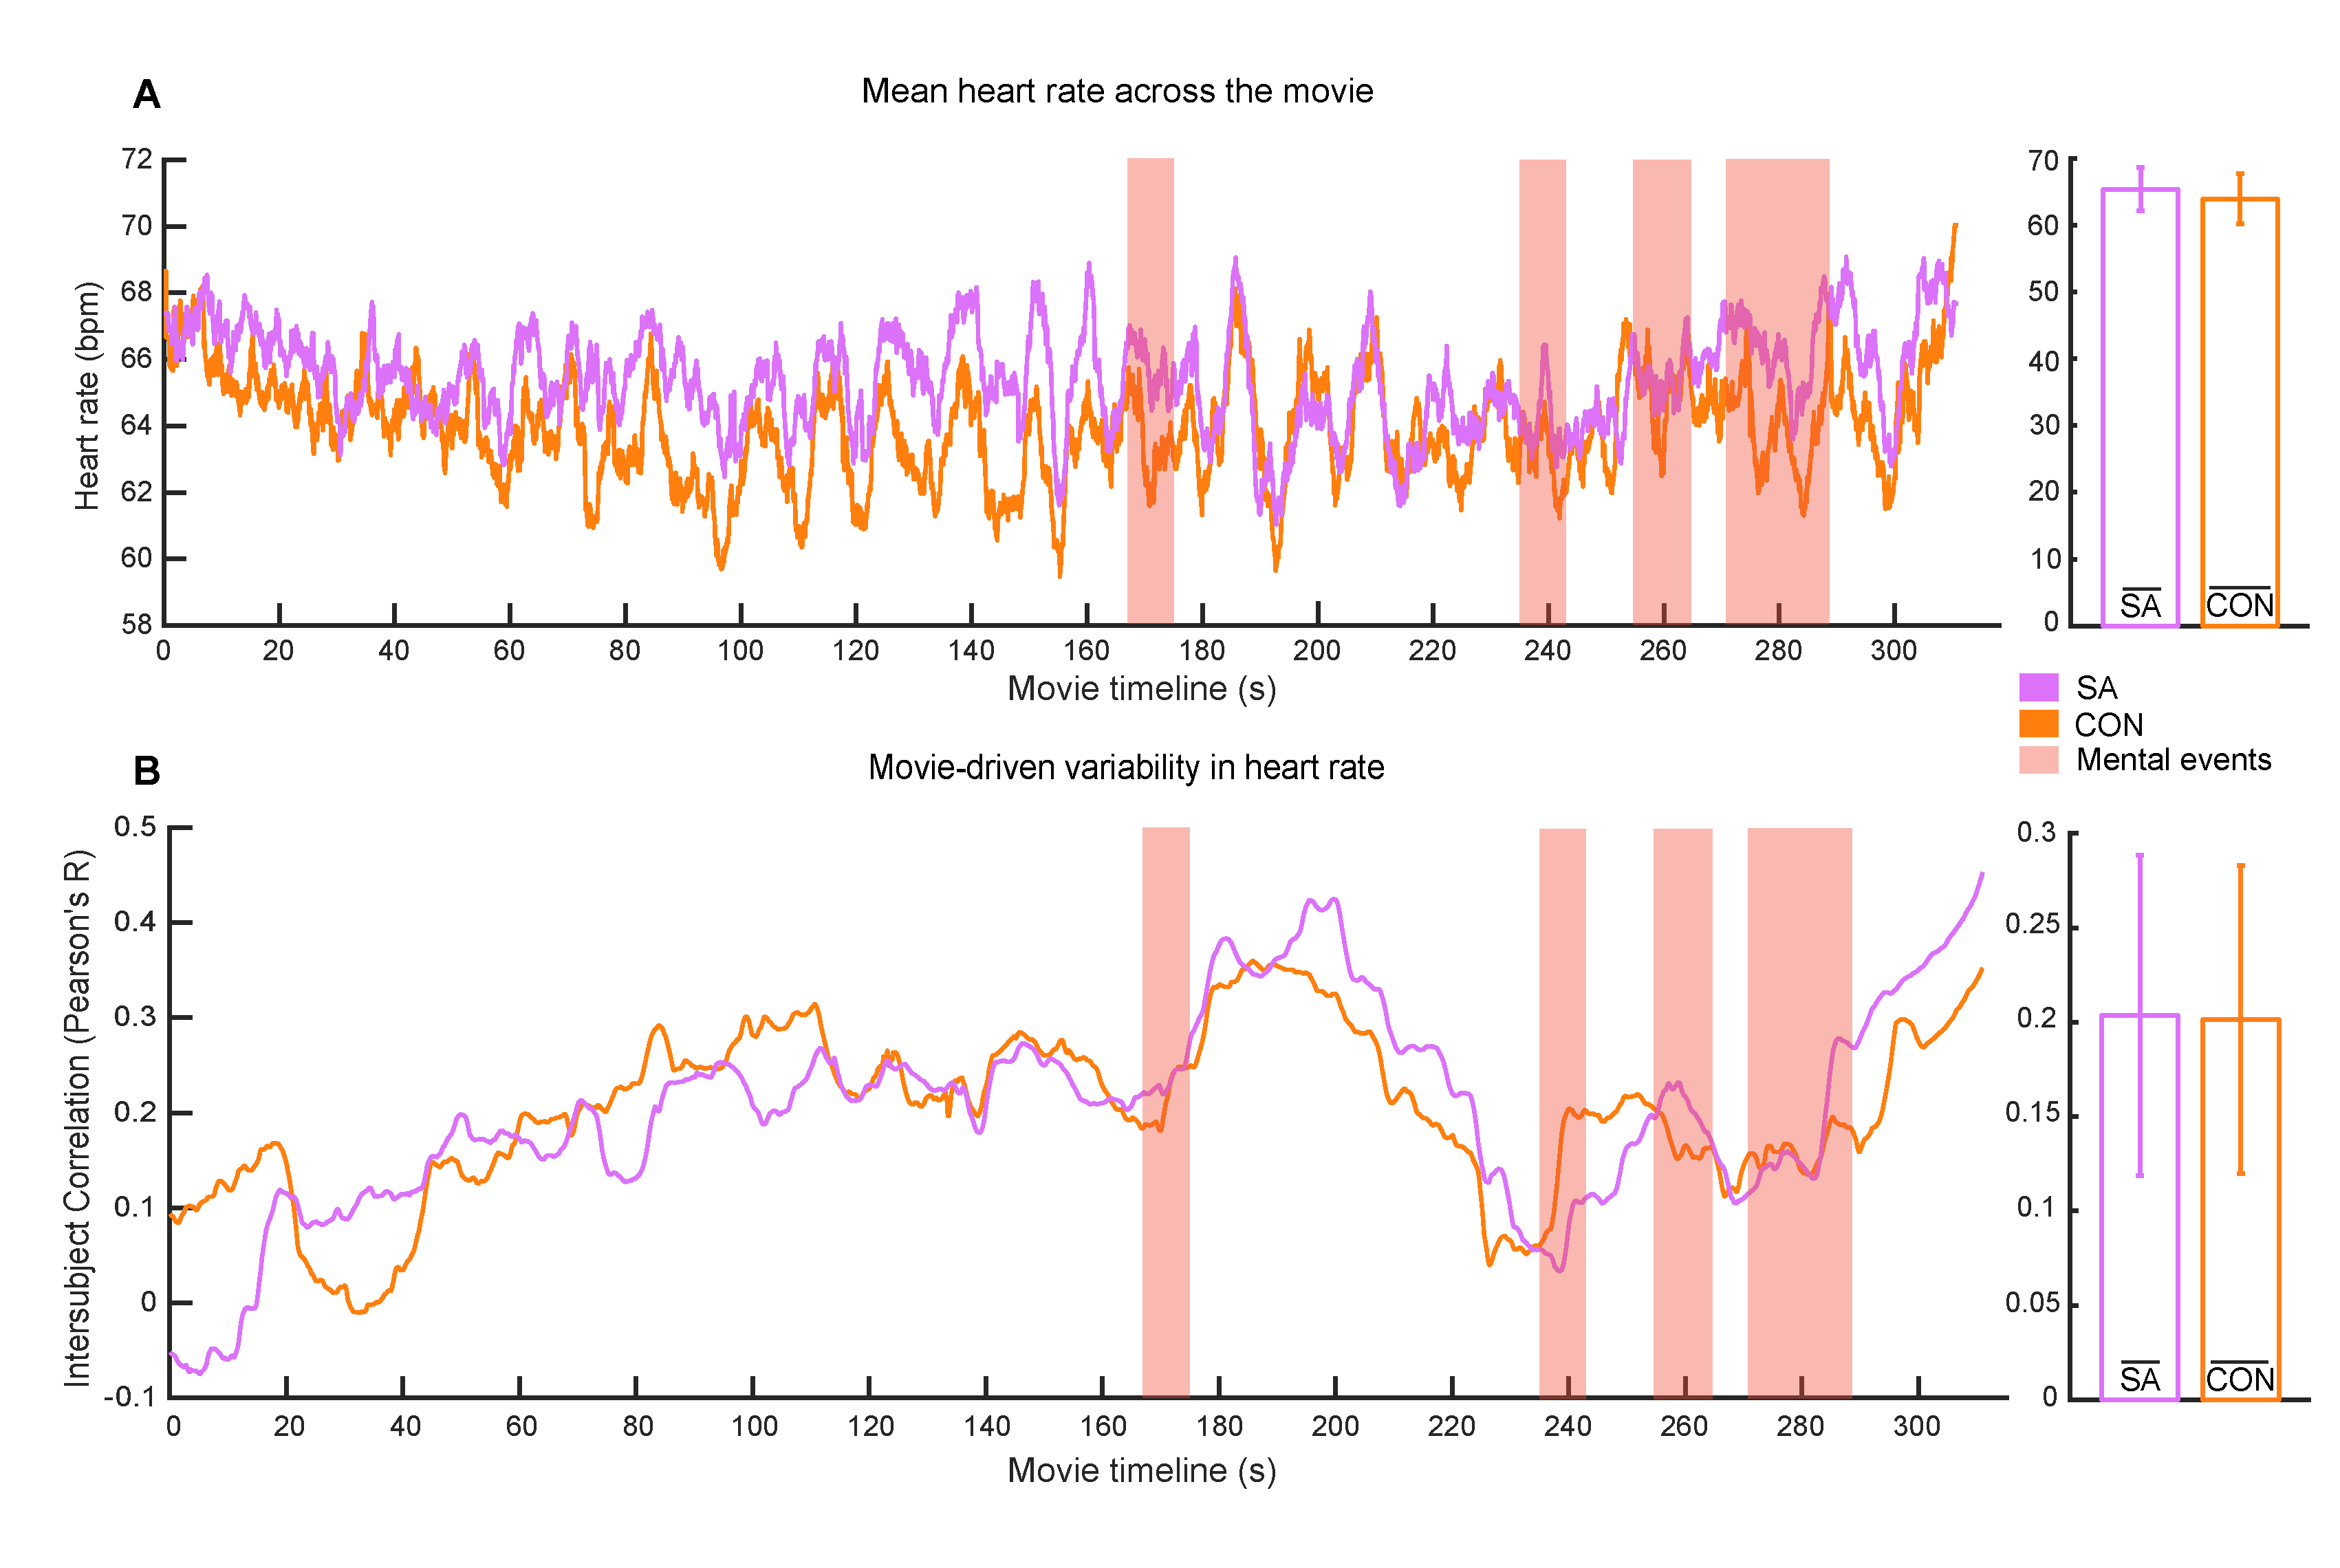
\includegraphics[width=1\textwidth]{./Chapters/03_MentalizingSA/Images/HeartRate.eps}}
	\caption{(a) Mean heart rate measured across the duration of the movie for both socially anxious and control participants. Adjacent histograms show the aggregated mean heart rate throughout the entire film for each group, with error bars representing 95\% confidence intervals. (b) Average intersubject correlation coefficients illustrate the intersubject variability in heart rate response during the movie among socially anxious and control participants. There were no significant differences detected in either metric between the two groups.}
    \vspace*{-10pt}
	\label{fig:heart-rate}
\end{figure}



\vspace{10pt}

\begin{figure}[!t]
	\centering
    \makebox[\textwidth][c]{\includegraphics[width=1\textwidth]{./Chapters/03_MentalizingSA/Images/ISCPupil.eps}}
	\caption{Dynamic intersubject correlation analysis revealed substantial fluctuations in variability throughout the film. Socially anxious participants exhibited lower correlations, indicative of higher variability in pupil responses compared to controls. Nonetheless, these differences did not reach statistical significance at any point during the viewing.}
    \vspace*{-10pt}
	\label{fig:isc-pupil-sa}
\end{figure}



\afterpage{\blankpage}
\chapter[Oscillatory Language Dynamics in Autism]{As the Sentence Unfolds: Oscillatory Dynamics of Language Processing in Verbally Competent Autistic Adults}
\label{ch:language_asc}

\begin{center}
    \large\textit{Abstract}
\end{center} 

{\abstractfont 
Autistic individuals often experience challenges and delays in language development, yet it remains unclear whether their language processing unfolds differently from that of neurotypical individuals in adulthood. In this study, we used EEG to examine real-time oscillatory neural dynamics as autistic adults and verbally and age-matched neurotypical controls read both structured sentences and pseudoword lists. Comparing these two conditions in reading revealed systematic spatiotemporal power dynamics across theta, alpha, beta, and gamma frequency bands across participants. These patterns included high power in the beta band during sentence reading and a progressive intensification of this beta signature as sentences unfolded, indicating cumulative processing of linguistic structure. Importantly, these oscillatory patterns appeared consistent across both autistic and neurotypical participants, with current analyses revealing no statistically significant differences in spatiotemporal progression or lateralization between groups. These findings suggest that sentence-level linguistic processing unfolds neurophysiologically in a similar manner in verbally competent autistic adults, suggesting that other underlying factors may contribute to language developmental delays in autism. \par
} 

\vspace*{\fill} 

\thispagestyle{empty}

\newpage

\section{Introduction}

Delays in language development are a common feature of autism, with approximately one-third of individuals remaining minimally verbal throughout their lives \citep{apa2013,kim2014,velikonja2019}. Although not a diagnostic criterion, autism is often first recognized due to atypical or delayed patterns of speech development during the second year of life, when most children of the same age begin to establish vocabularies comprising numerous words \citep{short1988}. However, such delays in expressive language during early preschool years are not unique to autism, and some individuals with autism acquire language typically despite marked social deficits \citep{anderson2007}. These observations underscore the complexity of language development in autism, highlighting the need to investigate whether language processing is fundamentally different, potentially involving distinct neural mechanisms even in verbally competent adults, or whether other underlying factors are responsible for the observed delays in language acquisition.

In search of a possible biomarker of autism and the associated language difficulties, a multitude of studies have been performed on the neural underpinnings of language processing in autism. Reduced neural activation to language and auditory stimuli has been found in brain regions typically involved in language \citep[for reviews]{groen2008,philip2012}. These results, however, are not always consistent \citep{tryfon2018}. A crucial challenge in interpreting these findings is that most studies depend primarily on neuroimaging techniques like fMRI, which restricts our insight into the neurophysiological processes involved in linguistic comprehension in autistic individuals. 

Electrophysiological investigations into language processing can provide insights on the mechanisms involved and their time course. These mechanisms operate at different frequencies that reflect circuit-level functions. These electrophysiological studies, however, are scarce in the current literature. A pair of studies investigated this in neurotypical individuals by having participants read sentences or pseudoword lists in an RSVP (Rapid Serial Visual Presentation) paradigm and applying Electroencephalography (EEG) and Magnetoencephalography \citep[MEG;][]{bastiaansen2010,bastiaansen2015}. This sentences vs. pseudoword list contrast probes the word-by-word operation of building a sentence-level representation, known as linguistic structure building. Firstly, they showed that higher power in the beta band was elicited at sensors over central, frontal, and bilateral parietal brain areas in response to linguistic structure building, as well as higher power in the theta band at sensors over right parietal areas. In terms of the time course of these effects, both studies found increasingly large beta and theta power differences between structure building and non-structure building conditions over the course of the sentence. Increases in beta and alpha power during linguistic structure building are suggested to reflect the maintenance of the sentence-level representation \citep{engel2010,lewis2016}, while theta may be linked to keeping sequentially ordered information in working memory \citep{roux2014,vignali2016}. In the gamma band, intracranial findings showed a ramping increase in power across the sentence structure \citep{fedorenko2016}, possibly reflecting (visual) information held in working memory \citep{bastos2018,honkanen2015,roux2014,vignali2016}. Whether these neural mechanisms are different in autistic individuals, is still an open question.

A more common finding for the neural basis of language processing in autistic individuals is reduced left-lateralized activation, often a consequence of increased involvement of the right hemisphere during language processing \citep{herringshaw2016}. This phenomenon was observed in semantic processing \citep{knaus2008}, lexico-semantic processing \citep{coffeycorina2008}, phonological processing \citep{dawson1986}, and sentence processing \citep{muller1999}. A recent, relatively well-powered study on linguistic structure building found reduced left-lateralization in autistic individuals using a similar linguistic structure building contrast as in the Bastiaansen et al. studies \citep{jouravlev2020}. Given the fact that most of these studies on the lateralization of language processing used fMRI, it is an unresolved question whether differences in lateralization in autism have a temporal component, i.e., whether they occur early or late during linguistic structure building. This research on lateralization is of clinical relevance because lateralization during language processing and measures of language ability are uniquely correlated in autistic individuals \citep{lindell2013}. Thus, findings could provide clues regarding the cause of autism-specific language difficulties. 

Considering the replicated findings in the two studies by Bastiaansen et al., the beta power increases provide a useful neural marker of structure building across the sentence. This marker can consequently be used to examine and compare structure building between autistic and neurotypical individuals, in addition to the degree of lateralization of structure building. Therefore, our aim for this study was to investigate the oscillatory activity during linguistic structure building, in particular the beta band, in autistic and neurotypical individuals. To tap into this broad linguistic process, we used the sentences vs. pseudoword list contrast from \cite{jouravlev2020}. First, higher beta power for sentences (linguistic structure building) compared to pseudoword lists was expected based on the findings from previous studies using this contrast \citep{bastiaansen2010,bastiaansen2015}, and this difference was expected to increase as the sentences unfold. Again based on previous work, we predicted that these effects would be maximal at electrodes over parietal regions. Given the inconsistent findings, we had slight expectations for stronger beta power in autistic individuals, although this is based on findings using different techniques and contrasts \citep{philip2012}. A second aim of our study was to investigate the degree of left-lateralization of power, in particular the beta band as an index of linguistic structure building, and its progression over time. This left-lateralization was calculated to compare between autistic and neurotypical individuals. Since one of the key motivations for using EEG was to observe potential temporal dynamics related to degree of lateralization in autistic vs neurotypical individuals, the beta power lateralization was computed and compared across time in one-second windows. Afterwards, these lateralization  indices were compared separately at each of these time points between autistic and neurotypical groups, and compared on their rate of linear increase or decrease. We expected beta power to be more left-lateralized in neurotypicals compared to autistic individuals, following the fMRI literature showing differences between the two groups. Moreover, this difference in lateralization of beta power between groups may reasonably be expected to be larger at later time points after there has ostensibly been more time for structure building to take place. By analyzing these oscillatory dynamics, we seek to determine whether linguistic structure building is altered in autism, shedding light on its potential role as a source of communicative variability in autistic individuals.

\section{Materials and methods}

\subsection{Participants}
Forty autistic individuals (ASC) were included in this study on the basis of having a diagnosis of Autism Spectrum Disorder, as well as 36 neurotypical (NT) individuals. They were recruited from advertisements on social media, posters on campus, and Radboud University's participant database. They were included as autistic participants if they had an official diagnosis by a qualified clinician \citep{apa2013}, which was further validated by their scores on the Autism-Spectrum Quotient questionnaire \citep[AQ]{baron-cohen2001AQ}. The autistic participants can be classified as high-functioning given the low support demands in their daily lives. Exclusion criteria for all participants constituted severe cognitive impairment, systemic disease, a history of neurological impairment, and the use of psychotropic medication or systemic glucocorticoids. Each participant performed the experiment while EEG data was collected, after which the participants filled out a questionnaire with questions and tasks assessing a.o. their IQ, handedness, and autistic traits \citep{baron-cohen2001AQ,raven1989,veale2014}. Eight additional individuals participated in the study but their EEG data were not included in the study. The data of four of these participants were excluded due to technical malfunctions during the session. The other four participants' data were excluded due to poor data quality, for which less than 20 trials per condition were included after artifact rejection, or a full coverage of the head could not be established due to rejected bad electrodes. All participants gave written informed consent for the study protocol, which was approved by the local ethics committee (CMO region Arnhem-Nijmegen, file number 2019-6059). Participants were all compensated for their time investment and their travels.

The autistic and neurotypical individuals were matched on age, gender, handedness, and both verbal and non-verbal IQ (see Table~\ref{tab:ppt-stats-lang}). Statistical tests did not reveal differences between the autistic and neurotypical groups on gender balance (55.0\% vs. 44.4\% women, \textit{$\chi$\textsuperscript{2}} (1, \textit{N} = 76) = 0.48, \textit{p} = .49), on age (M \textpm{} SD 28.9 \textpm{} 6.8 vs. 27.0 \textpm{} 5.6, \textit{t}(74) = 1.29, \textit{p} = .20), on handedness (M \textpm{} SD 69.6 \textpm{} 69.8 vs. 84.7 \textpm{} 51.9, \textit{t}(74) = -1.15, \textit{p} = .25), or on verbal IQ measured by the Vocabulary and Similarities subscales of the Wechsler Adult Intelligence Scale \citep[128 \textpm{} 7 vs. 128 \textpm{} 16, \textit{t}(74) = -0.07, \textit{p} = .95]{wechsler1997} and performance IQ measured by the timed version of the Raven's Progressive Matrices test \citep[102 \textpm{} 9 vs. 103 \textpm{} 14, \textit{t}(74) = -0.35, \textit{p} = .73]{raven1989}. The Autism-Spectrum Quotient, as expected, showed a large difference between autistic and neurotypical participants (30 \textpm{} 9 vs. 14 \textpm{} 6, \textit{t}(74) = 9.23, \textit{p} <  .001), validating the distinction between the two groups.

\begin{table}[ht]
    \captionsetup{justification=raggedright, singlelinecheck=false, font = normal} % Left-align the caption
    \setlength{\tabcolsep}{7.5pt} % Adjust column spacing if needed
    \renewcommand{\arraystretch}{1.5} % Adjust row spacing
    \caption{Demographic data}
    \label{tab:ppt-stats-lang}
    \begin{tabular}{llll}
    \hline
    \textbf{} & \textit{ASC Group} & \textit{NT Group} & \textit{Group Difference} \\
    \hline
    N (women:men) & 40 (22:18) & 36 (16:20) & \textit{$\chi$\textsuperscript{2}}(1, N = 76) = 0.48, \textit{p} = .49 \\
    Age (years) & 28.9 (6.8) & 27.0 (5.6) & \textit{t}(74) = 1.29, \textit{p} = .20 \\
    Handedness (EHI) & 69.6 (69.8) & 84.7 (51.9) & \textit{t}(74) = -1.15, \textit{p} = .25 \\
    Verbal IQ (WAIS-III) & 128 (7) & 128 (16) & \textit{t}(74) = -0.07, \textit{p} = .95 \\
    Non-verbal IQ (RPM) & 102 (9) & 103 (14) & \textit{t}(74) = -0.35, \textit{p} = .73 \\
    Autism Quotient & 30 (9) & 14 (6) & \textit{t}(74) = 9.23, \textit{p} < .001 \\
    \hline
    \multicolumn{4}{l}{\footnotesize{Values are given as Mean (Standard Deviation). ASC, Autism Spectrum Condition; NT, Neurotypical.}} 
    \end{tabular}
\end{table}

\subsection{Experimental design}
Neural responses to linguistic structure building were assessed with a reading paradigm based on \cite{fedorenko2010}, contrasting two conditions: sentences and pseudoword lists. Sequences in both conditions contained twelve words or pseudowords, presented serially at a rapid pace. The sentences and pseudoword lists were matched in the number of letters and syllables (letters: M\textsubscript{SEN} (SD\textsubscript{SEN}) = 72.5 (5.8), M\textsubscript{LIST} (SD\textsubscript{LIST}) = 72.6 (6.2); syllables: M\textsubscript{SEN} (SD\textsubscript{SEN}) = 20.7 (2.1), M\textsubscript{LIST} (SD\textsubscript{LIST}) = 20.8 (2.2)) and the topics described in the sentences were varied. The pseudoword lists were created by replacing the content words in the sentences with pseudowords, and scrambling all (function) words and pseudowords in the sentence. Two independent native Dutch raters confirmed that the pseudowords did not resemble existing Dutch words. To ensure that participants were closely reading all sequences, they were given a memory task to answer whether a probe word was presented in the sequence they just read. All sequences were presented in a randomized order for each participant, and presented in blocks of three sequences for each condition. Before each block, a fixation cross was presented for a random duration between 4000 and 7750 milliseconds. Before each sequence, a fixation cross was presented for 200 milliseconds. Each word or pseudoword was presented for 400 milliseconds. After the sequence, the memory probe word of the task was presented for 750 milliseconds. These durations are specified for the experiment presentation software, but the screen refresh time is added to these durations. For a subset of the participants in this study, the screen refresh times were 33 ms longer due to changes following hardware replacement. Importantly, the proportion of participants with different screen refresh durations is exactly the same between groups (75\% longer and 25\% shorter durations for both groups), ruling out the possibility of this difference explaining group effects. This difference is further corrected for in the data analysis section (see section \ref{preprocessing}). 

\begin{table}[ht]
    \captionsetup{justification=raggedright, singlelinecheck=false, font = normal} % Left-align the caption
    \renewcommand{\arraystretch}{1.5} % Adjust row spacing
    \caption{Example sequences for the two conditions with English translation.}
    \label{tab:example_sequences}
    \small
    \begin{tabular}{lp{8.2cm}}
    \hline
    \textit{Condition} & \textit{Example item} \\
    \hline
    \small{SENT (sentence)} & \small{Meer dan duizend arbeiders werken in het moderne bedrijf tegenover het station.} \\
     & \small{\textit{More than a thousand employees work at the modern company across from the station.}} \\
    \small{LIST (pseudoword list)} & \small{van eingelzing bepen camzen parpisch uit naar groden kastren van naar moemels} \\
     & \small{\textit{from} eingelzing bepen camzen parpisch \textit{out to} groden kastren \textit{of to} moemels*} \\
    \hline
    \multicolumn{2}{l}{\footnotesize *Only translations for existing Dutch function words.} \\
    \end{tabular}
    \normalsize
\end{table}

\begin{figure}[!ht]
	\centering
    \makebox[\textwidth][c]{\includegraphics[width=1\textwidth]{./Chapters/04_LanguageASC/Images/ExpDesign.eps}}
	\caption{Schematic of the task performed by autistic and neurotypical participants during the EEG experiment to ensure a close reading of the sequences. Sentences (shown here) or pseudoword lists were presented by showing every word or pseudoword consecutively for 400 ms, preceded by a fixation cross for 200 ms. After each sequence, participants were asked whether a target word (here: \textit{station}), on screen for 750 ms, was shown in the sequence they had just read, which they indicated via button press.}
    \vspace*{-10pt}
	\label{fig:exp-design}
\end{figure}




\subsection{Procedure}
Measurements took place in an electrically-shielded, sound-proof room. Before the EEG preparation started, participants were informed about the steps of the EEG preparation and measurement procedures. They received instructions about the task, including having to answer whether the probe word was part of the sequence that was presented before. They were instructed to use their left index finger to press a left button for yes and their right index finger to press a right button for no. They were also informed that while the reading and task decision tempo was quite high, their response would still be registered if they pressed the button after the probe word disappeared from the screen. Lastly, they were instructed to minimize head movement as much as possible during the task. The participants rested their head on a head and chin rest, reducing head movement, with a viewing distance of 59 cm. The words and pseudowords in the sequences and fixation crosses were presented in black text in the center of the screen with a light grey background. All text was presented in the Courier New font with size 18. Both the target word and `yes' and `no' were presented in red text. The measurement lasted for 12 minutes. 

\subsection{EEG recordings}
A fitting 64-electrode actiCap with active sensors was placed on participants' heads. The left mastoid electrode was used as a reference and an electrode at the center of the forehead as a ground electrode. To measure vertical eye movements, two electrodes were placed at the supra- and suborbital ridges of the right eye. For horizontal eye movements, two electrodes were positioned in a right-to-left outer canthal bipolar montage. Electrode impedance was kept below 25 kilo-ohms during the experiment. EEG data were amplified and collected with BrainAmp DC amplifiers at a sampling rate of 5000 Hz with a 0.1 - 1000 Hz band-pass filter. 

\subsection{Behavioral analysis}
To check whether participants were sufficiently engaged in the experiment, response rate for the memory task was calculated for each participant. With an independent \textit{t}-test (\textit{alpha} = 0.05) we assessed whether autistic and neurotypical individuals responded to a similar number of trials. Reaction time and accuracy to the memory task was recorded in order to compare the difficulty of the task between conditions and groups. To capture the variability in performance across trials and subjects, generalized linear mixed effects models in R (version 4.3.3) were used to investigate reaction time and accuracy with the \textit{lme4} package \citep{bates2015}. For modelling reaction time, participant group (autistic or neurotypical) and condition (sentence or pseudoword list) were included as fixed effects with their interaction term, together with a subject-specific intercept as random effect. This reaction time model was created to assume an inverse gaussian distribution with a log link function, optimized to only fit positive data \citep{lo2015}. The same model structure of fixed and random effects, but with a binomial distribution and a logit link function, was used to calculate effects for accuracy. Significance of the effects was identified with the \textit{lmerTest} package \citep{kuznetsova2017}, which uses Satterthwaite's method to calculate \textit{p}-values.

\subsection{EEG Preprocessing} \label{preprocessing}
EEG data were analyzed using the Fieldtrip toolbox \citep{oostenveld2011} in a MATLAB environment (R2020a; Mathworks, Inc.). The data were processed with a low-pass filter at 199 Hz and a band-stop filter at 50, 100 and 150 Hz to reduce effects of power line noise (50 Hz). Artifact rejection was done in two stages of visual inspection of the data. First, the continuous EEG data were visually inspected for blinks, eye movements and high-frequency noise. Segments containing these artifacts were replaced with zeros. At trial definition, trials with less than two seconds of included data were excluded from further analyses. Afterwards, trials and channels containing noise and artifacts were rejected from the data on the basis of amplitude variance and kurtosis (all measured per trial across time). All scalp electrodes were re-referenced to the common average reference. Bad channels were repaired by reconstructing them from the average of their neighbouring channels. After artifact rejection, 19\% of all trials were excluded. Importantly, the number of rejected trials was comparable for the two conditions (M\textsubscript{SEN} = 19.2\%, M\textsubscript{LIST} = 17.8\%, \textit{t} (75) = 1.36, \textit{p} = .18) and the autistic and neurotypical groups (M\textsubscript{ASC} = 18.4\%, M\textsubscript{LIST} = 18.6\%, \textit{t} (75) = -0.09, \textit{p} = .93). Finally, all data were segmented from -300 ms to 5500 ms relative to the onset of the first word in the sequence. This trial duration was chosen as it corresponds to the shortest trial across all participants. Because of this procedure, the analysis excludes the last 396 ms of longer trial durations that are due to longer screen refresh times (12 (pseudo)words * 33 ms of screen refresh duration = 396 ms). This procedure was done to be able to include data from participants with both shorter and longer screen refresh times. Crucially, power changes in the sentence vs. pseudoword list contrast were not different for participants with short or long screen refresh times (see Supplementary Note \ref{suppl-note}).

\subsection{Sentences vs. pseudoword lists power and statistical analysis}
Time-frequency spectra were calculated for each trial separately using a sliding-window approach with a Hanning taper and the application of a fast Fourier transform. Frequencies were estimated between 2 and 100 Hz in steps of 2 Hz with a sliding window of 500 ms applied in steps of 20 ms. The sliding window length was chosen in order to optimize sensitivity in the beta band, the frequency band of interest, which tends to be relatively short-lived \citep{jones2016}. This means that the power in every time-frequency point represents a weighted average of -250 ms to 250 ms at the specified timepoint. Power values were then expressed as a relative change from the standard deviation of the power of all trials. This \textit{z}-scoring was done over all trials of both conditions within the full time window. This was performed separately for each channel, frequency, and time bin and resultant \textit{z}-scored power values were then averaged across trials. 

To calculate and compare power changes between the sentence and pseudoword list conditions, statistical testing was performed with cluster-based random permutation testing on power changes in the two conditions averaged over trials \citep{maris2007}. This method was chosen because it elegantly handles the multiple comparisons problem. Briefly summarized, for every data point (electrode-frequency-time point) a dependent \textit{t}-test is performed which generates uncorrected \textit{p}-values. These are compared against a pre-set significance level (here, 5\% two-tailed) and data points at which \textit{p}-values fall above this level are discarded. The remaining data is used to form clusters based on their adjacency in space (channels), frequency, and time. Cluster-level statistics are then computed by summing the \textit{t}-values of the data points that make up each cluster. Next, a permutation distribution is created by randomly assigning participant averages to one of the two conditions, an approach that is repeated 5000 times. Each permutation, cluster-level statistics are calculated, with the highest cluster-level statistic included in the permutation distribution. The cluster statistic for the measured data was compared against this distribution, and clusters that fell in the lowest or highest 2.5\% of the distribution were considered statistically significant. Statistical testing was first performed over the full frequency range between 2 and 100 Hz, allowing both spatial and spectral clustering for multiple comparison correction. Afterwards, the effects were separately tested in theta (3 - 7 Hz), alpha (7 - 13 Hz), beta (14 - 20 Hz) and gamma (60 - 80 Hz), averaged over the specific frequency band. The time window for which we tested the data was from 0 to 5200 ms relative to the onset of the first word of the sequences. Reported effect sizes for the cluster on the basis of which the H0 was rejected, were calculated by averaging over the data in this cluster. 

For a between-group comparison of power changes during linguistic structure building, the power difference between the sentence and pseudoword lists was calculated by subtracting the grand averages of the pseudoword lists condition from the sentences condition for each subject. Power changes were then compared between autistic and neurotypical individuals with cluster-based permutation testing using independent \textit{t}-tests (\textit{alpha} = 0.05). Bayes Factors were computed for between-group differences in power changes in peak channels and timepoints to assess the evidence for the null model and the model that specifies group.

To more sensitively assess whether this contrast, ostensibly designed to probe linguistic structure building, is constant or changes over time, a second test was performed.  For this test, a linear regression model across trial time course was fit to the power for each subject, condition and frequency band at its peak channel. These subject-specific regression fits were then compared between autistic and neurotypical individuals and sentence and pseudoword list conditions in an ANOVA with group, condition and their interaction as independent variables. 

\subsection{Laterality index}

For comparing lateralization of the linguistic structure building effect in the brain between groups and its progression over time, the previously calculated power values were split into five time windows of one second, spanning the trial time course, and averaged over these windows and over each of the four frequency bands. For these frequency bands and the five time windows, the difference in power between the sentence and pseudoword list conditions was calculated as the normalized power difference as the following: (SENT - LIST) / (SENT + LIST). This normalization was done to take into account electrodes that have differing levels of signal strength or quality. A laterality index for these power differences was calculated for all non-midline electrodes by subtracting the power of the right electrode from the power of the left electrode (Left - Right). This resulted in values representing the extent of the left-lateralization of the power difference for each electrode pair. While lateralization is more commonly calculated by dividing this Left-Right electrode difference by the sum of these two power values, this would lead to extreme values due to possible negative and positive values in the denominator. For this reason, we chose to exclude the denominator from the calculation. Note that these values represented the effects picked up on the scalp and not the precise location of the underlying neural generators due to volume conduction.

Grand averages of the laterality index were computed for each frequency band across time. To determine whether time-frequency power in the four frequency bands was lateralized in the first place, the laterality indices were compared to zero with the aforementioned cluster-based permutation method using dependent \textit{t}-tests (\textit{alpha} = 0.05). This was done for the autistic and neurotypical group separately. Crucially, the lateralization of power during linguistic structure building were then compared between the autistic and neurotypical participant groups with a cluster-based permutation method using independent \textit{t}-tests (\textit{alpha} = 0.05). This comparison of lateralization index between groups was chosen because it mirrors the approach of the fMRI study which found group differences in lateralization of the sentences vs. pseudoword lists contrast \citep{jouravlev2020}. The beta band was of particular interest in this analysis on account of previous studies showing it is the strongest index of linguistic structure building \citep{bastiaansen2010,bastiaansen2015}. 

To additionally assess group differences in language laterality more sensitively, we identified four electrodes where the sentence vs. pseudoword list contrast from the previous analysis was strongest across groups. These electrodes were therefore identified independently of the whole-brain laterality analysis. In these four peak electrodes, the average laterality index was calculated for each frequency band and time window. To determine whether power during linguistic structure building was lateralized in the first place, these average laterality indices were first compared against zero in both groups. This comparison was done with dependent \textit{t}-tests Bonferroni-corrected for the number of time windows (\textit{alpha} = 0.01). Afterwards, the laterality indices were compared between autistic and neurotypical participants with an independent \textit{t}-test (\textit{alpha} = 0.01), and Bayes Factors were computed and reported to assess the evidence for the null model or the model that specifies group status.

Finally, to statistically evaluate the time course of the laterality, a subject-specific linear regression model was fit to the laterality indices, mirroring the procedure for the power values. These regression fits were first compared against zero to determine whether lateralization in the four frequency bands varied over time. To investigate the difference in laterality time course for autistic and neurotypical individuals, the subject-specific regression fits on laterality values were subsequently compared in an independent \textit{t}-test (\textit{alpha} = 0.05). 

\section{Results}
\subsection{Behavioral task}
When asked if a word or pseudoword was part of a sentence or a list they read, responses were logged for 95.2\% of the trials on average (SD = 10.4\%), meaning participants did not respond to 4.8\% of the trials or responded too late. In addition, no participants responded to less than 50\% of trials and most participants (60\%) responding to all or all but one of the trials. These results indicate that participants attended to the task at hand. Response rates were within the same range for autistic and neurotypical individuals (M\textsubscript{ASC} = 94.2\%,  M\textsubscript{NT} = 96.5\%; \textit{t} (74) = -0.97, \textit{p} = .33), showing that the participant groups are similarly engaged with the task. In terms of analyzing response performance, we found that 82.5\% of trials were answered correctly on average (SD = 12.2\%). Much higher accuracy was found for responses for sentences than for pseudowords (M\textsubscript{SEN} = 89.8\%,  M\textsubscript{LIST} = 75.2\%; beta = 1.62, SE = 0.12, \textit{z} = 13.2, \textit{p} <  .001). A similar pattern was apparent for reaction times: participants took an average of 706 ms to respond (SD = 112.9 ms), but were much faster when responding to sentences than to pseudoword lists (M\textsubscript{SEN} = 657.9 ms,  M\textsubscript{LIST} = 754.1 ms; beta =  -0.13, SE = 0.01, \textit{t} = -17.7, \textit{p} <  .001). When comparing response measures between groups, we see that autistic and neurotypical individuals were equally accurate in task performance  (M\textsubscript{ASC} = 82.5\%,  M\textsubscript{NT} = 82.5\%; beta = -0.11, SE = 0.17, \textit{z} =-0.68, \textit{p} = .50). Yet, autistic people were overall slower to respond than neurotypical participants (M\textsubscript{ASC} = 733.8 ms,  M\textsubscript{NT} = 675.1 ms; beta = 0.09, SE = 0.04, \textit{t} = 2.07, \textit{p} = .038). No interaction between participant group and task condition was found either for accuracy (beta = -0.27, SE = 0.17, \textit{t} = -1.61, \textit{p} = .11) or reaction time (beta = -0.01, SE = 0.01, \textit{t} = -0.52, \textit{p} = .61), which suggests that autistic participants show an equally large linguistic task effect as neurotypical individuals.


\subsection{Time Frequency Analysis}
\subsubsection{Sentences vs. pseudoword lists across and between groups}
Cluster-based permutation analyses showed that time-frequency power when reading sentences was significantly higher than when reading pseudoword lists in the full frequency range from 2 to 100 Hz (\textit{p} <  .001, \textit{d} = 1.33). The difference in power was present in all channels and time points up to 46 Hz (see Fig~\ref{fig:tf-spectrum-full}a). Analyses focused on the four frequency bands individually confirmed this difference between conditions for the beta (\textit{p} <  .001, \textit{d} = 1.81), alpha (\textit{p} <  .001, \textit{d} = 2.99), theta (\textit{p} <  .001, \textit{d} = 2.27) and gamma (\textit{p} = .03, \textit{d} = 0.42) bands.

\begin{figure}[!ht]
	\centering
    \makebox[\textwidth][c]{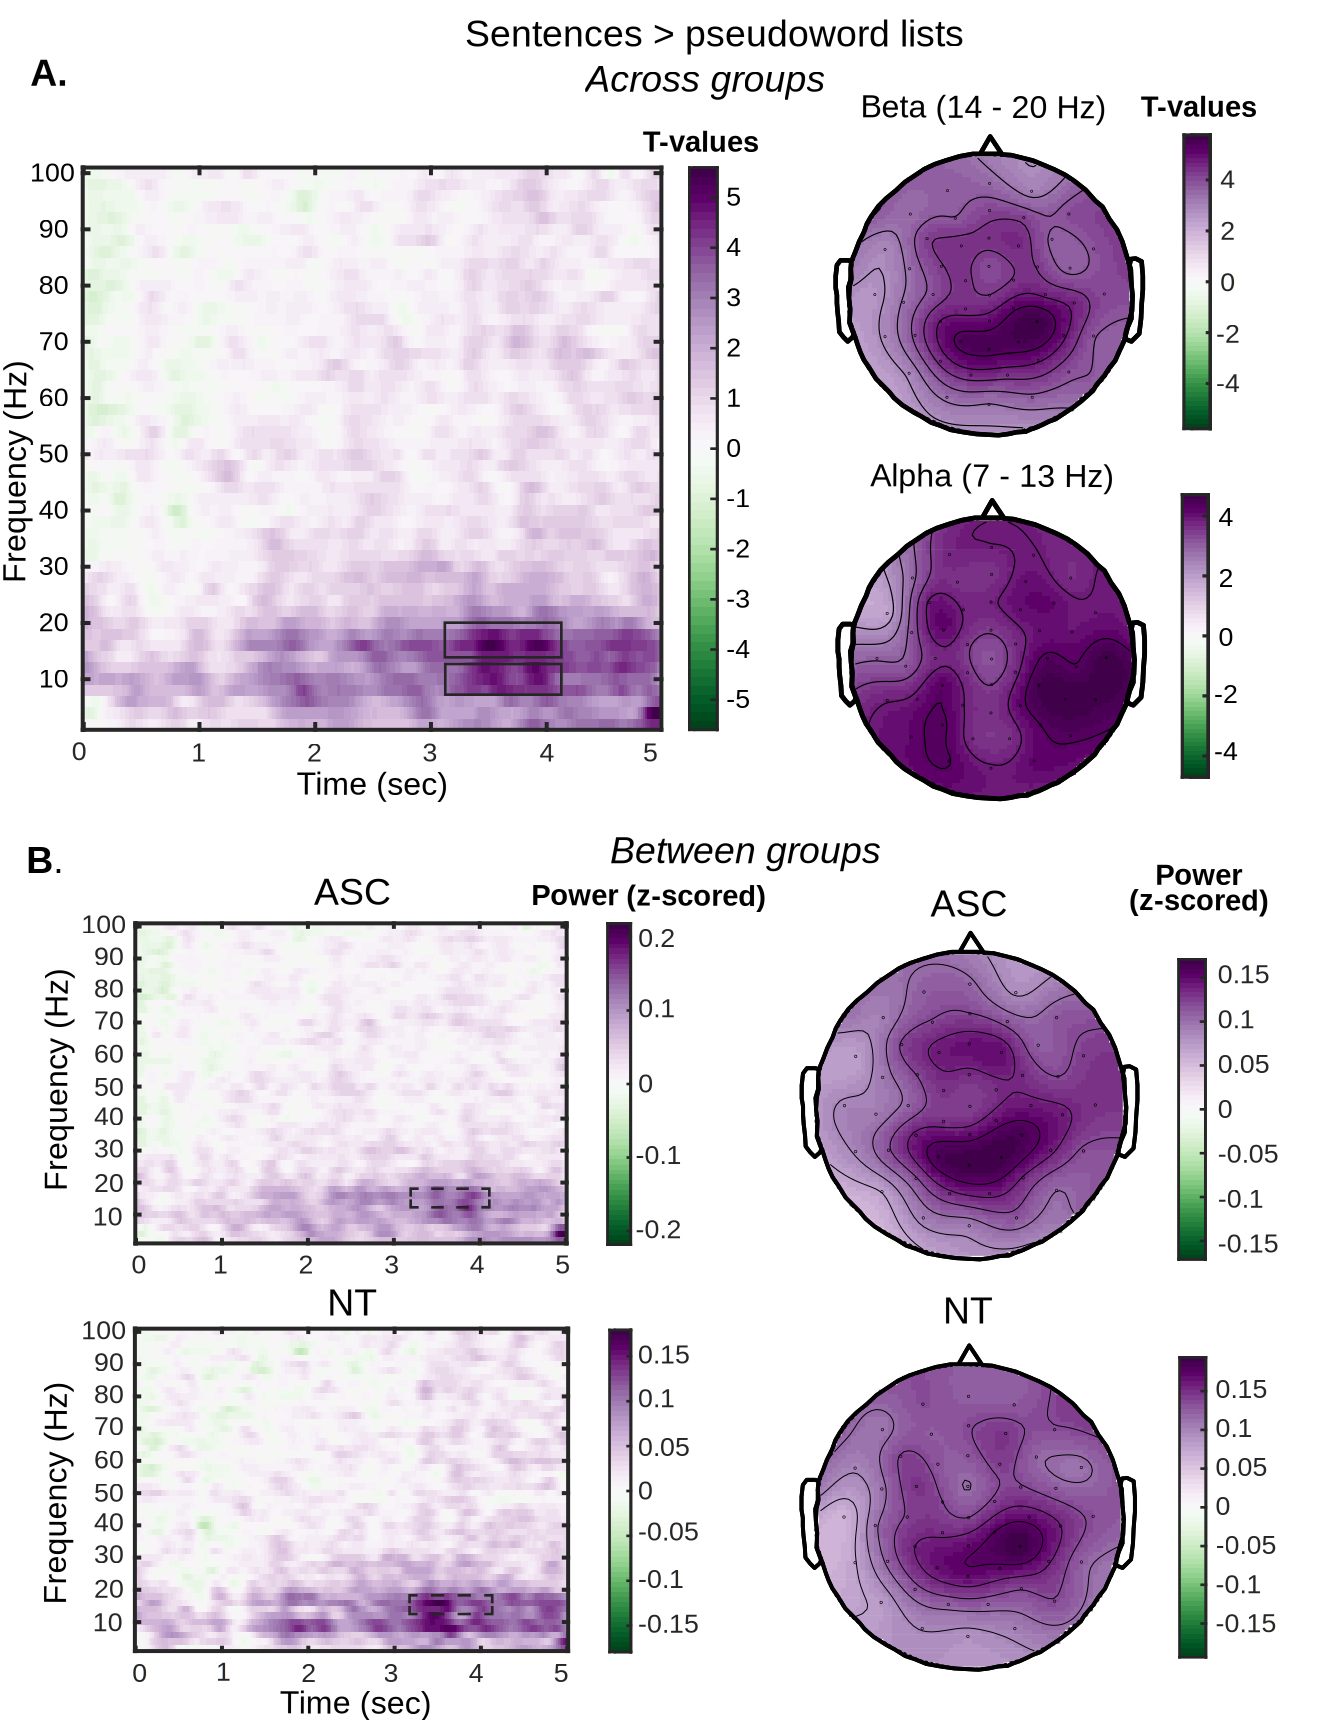
\includegraphics[width=.8\textwidth]{./Chapters/04_LanguageASC/Images/TFSpectrumFull_vert.eps}}
	\caption{Time-frequency (TF) dynamics in Sentences vs. pseudoword list contrast. (a) TF power is significantly different for the contrast, with power differences present across almost all channels, frequencies and timepoints. The color scale shows the relative difference in TF power (0 = no change). The timepoints and frequencies where the effect is strongest are indicated with boxes on the left, and the corresponding topography on the right for two different frequency bands: 14 - 20 Hz (beta) with bilateral posterior peaks, and 7 - 13 Hz (alpha) with a more widespread spatial effect. (b) TF power for the contrast was not different between neurotypical (NT) and autistic (ASC) participants. On the left, the similar TF spectra are shown, with the rectangle indicating the strongest power changes and on the right, the topography of this effect. }
    \vspace*{-10pt}
	\label{fig:tf-spectrum-full}
\end{figure}




The temporal dynamics of time-frequency power showed different patterns for the four frequency bands (see Fig~\ref{fig:tf-dynamics-topo}). The strongest power differences occurred in the latter part of the trial, peaking between 3 and 4 seconds after the onset of the first word, and in the beta band (around 16 Hz). This beta effect was primarily found at bilateral central posterior electrodes, peaking in the right hemisphere. Large power differences were also found for the alpha band (between 7 and 13 Hz), with a widespread spatial topography and strong effects at right parietal and left posterior electrodes. Given our experimental contrast, these alpha and beta differences likely contribute, at least partially and perhaps independently, to the cognitive process of linguistic structure building. 

\begin{figure}[!ht]
	\centering
    \makebox[\textwidth][c]{\includegraphics[width=1\textwidth]{./Chapters/04_LanguageASC/Images/TFDynamicsTopo.eps}}
	\caption{Time-frequency (TF) dynamics in Sentences vs. pseudoword list contrast across time and all participants for the theta (3 - 7 Hz), alpha (7 - 13 Hz), beta (14 - 20 Hz) and gamma (60 - 80 Hz) band.}
    \vspace*{-10pt}
	\label{fig:tf-dynamics-topo}
\end{figure}




Time-frequency power for this structure-building contrast was not significantly different between neurotypical and autistic individuals. The similar power spectra can be observed on the left hand side in Fig~\ref{fig:tf-spectrum-full}b, along with the topography of the strongest effect that was present in both groups. The similar time course of the two groups for both conditions can be seen in Fig~\ref{fig:tf-dynamics-peak}. A Bayesian analysis on the channels and timepoints showing maximal effects confirmed this lack of between-group differences for the beta (BF\textsubscript{NULL} = 3.31), alpha (BF\textsubscript{NULL} = 2.24), theta (BF\textsubscript{NULL} = 2.97) and gamma (BF\textsubscript{NULL} = 3.92) frequency bands. This indicates that oscillatory power in theta, alpha, beta, and gamma frequency bands during linguistic structure building are not different between neurotypical and autistic individuals. 

Subject-specific regression analyses indicated that progression of TF power over time was more positive while reading sentences compared to pseudoword lists in theta (\textit{d} = 0.48, \textit{p} = .004), alpha (\textit{d} = 0.46, \textit{p} = .005), and beta (\textit{d} = 0.96, \textit{p} <  .001; see Fig~\ref{fig:tf-dynamics-peak}a). This can be observed as the increasing difference in power over time between the conditions (see Fig~\ref{fig:tf-dynamics-peak}b). No significant difference between the condition in change over time was found for the gamma band (\textit{p} = .78). Time-frequency power change over time did not significantly differ for autistic and neurotypical participants in any of the four frequency bands, nor was there a significant interaction with condition. 

\begin{figure}[!ht]
    \vspace{10pt}
	\centering
    \makebox[\textwidth][c]{\includegraphics[width=.95\textwidth]{./Chapters/04_LanguageASC/Images/TFDynamicsPeak.eps}}
	\caption{Time-frequency (TF) power in the sentences and pseudoword lists (a) and difference of TF power between sentence and pseudoword list (b) across the trial time course for both groups. Power values are shown for the peak electrode in the sentences vs. pseudoword list contrast of the frequency band, of which the location is shown with scalp topography. Power differences over time between the two conditions were detected in the theta, alpha and beta band. No significant changes of TF power over time were found between autistic and neurotypical for any frequency band. Error bars indicate standard error. SENT = Sentences, LIST = Pseudoword lists. ** = \textit{p} < .001, * = \textit{p} < .01}
    \vspace*{-10pt}
	\label{fig:tf-dynamics-peak}
\end{figure}




\subsubsection{Lateralization of linguistic structure building}
Whole-scalp comparisons (all non-midline electrodes) were performed using cluster-based permutation statistics on the laterality indices of the sentences vs. pseudoword list contrast for the averaged one-second time windows and for the theta, alpha, beta, and gamma bands. Comparisons against zero in each participant group showed lower left-lateralization of power in the alpha band in the autistic individuals (\textit{p} = .002; see Fig~\ref{fig:laterality-topo}), driven by a cluster of frontal, lateral electrodes. No lateralized power was found in other frequency bands, nor in the neurotypical group. Despite this lateralization pattern in alpha, no differences in lateralization were found between autistic and neurotypical individuals in whole-brain comparisons for any of the four frequency bands. The similar lateralization patterns are shown across time in Fig~\ref{fig:laterality-dynamics-wholehem}.

\begin{figure}[!ht]
	\centering
    \makebox[\textwidth][c]{\includegraphics[width=1\textwidth]{./Chapters/04_LanguageASC/Images/LateralityTopo.eps}}
	\caption{Lateralization of time-frequency power in the sentences vs. pseudoword lists contrast detected across the hemisphere. Comparisons against zero showed significantly lower lateralization for autistic participants in the alpha band, driven by lateral electrodes. No significant changes of lateralization found between autistic and neurotypical for any frequency band. ** = \textit{p} < .01}
    \vspace*{5pt}
	\label{fig:laterality-topo}
\end{figure}




\vspace{.5cm}

\begin{figure}[!ht]
	\centering
    \makebox[\textwidth][c]{\includegraphics[width=.95\textwidth]{./Chapters/04_LanguageASC/Images/LateralityDynamicsWholeHem.eps}}
	\caption{Lateralization across the trial time course of time-frequency power in the sentences vs. pseudoword lists contrast for both groups averaged over the whole hemisphere. No significant changes of lateralization over time were found between autistic and neurotypical for any frequency band. Error bars indicate standard error. }
    \vspace*{-10pt}
	\label{fig:laterality-dynamics-wholehem}
\end{figure}


 

With a more spatially sensitive test, we inspected the topographies of the effects for the theta, alpha, beta, and gamma bands in the sentences vs. pseudoword list contrast, determined which electrodes showed maximal effects, and tested the laterality index between groups for these peak channels at each timepoint. For the beta, theta, and gamma band, independent \textit{t}-tests showed no statistically significant between-group differences in lateralization of the contrast at the selected electrodes in either of the five time windows (see Fig~\ref{fig:laterality-dynamics-peak}). This absence of group differences was corroborated by all Bayes factors for the null model being higher than for the model specifying group status (beta: BF\textsubscript{NULL} = 1.88 - 4.20, gamma: BF\textsubscript{NULL} = 2.63 - 4.13, theta: BF\textsubscript{NULL} = 1.82 - 4.13). For the alpha band, no significant between-group differences were found for four out of five timepoints (BF\textsubscript{NULL} = 2.39 - 4.19). There is evidence for a between-group difference in the alpha band between 1 and 2 seconds (BF\textsubscript{Group} = 1.4), although this difference did not pass the Bonferroni-corrected significance threshold (\textit{alpha}  = 0.01). These findings suggest that all frequency bands do not exhibit significant differential lateralization between neurotypical and autistic individuals during the process of linguistic structure building. 

After fitting a subject-specific linear regression model to the time course of lateralization during the sentence and pseudoword list conditions in the four peak channels, lateralization during linguistic structure building appeared stable across the trial, showing no deviating regression from zero (see Fig~\ref{fig:laterality-dynamics-peak}). Furthermore, lateralization was similarly stable for autistic and neurotypical individuals as no differences in time courses were found between the two groups. 

The analyses so far have regarded autistic and neurotypical individuals as separate categories, when autism can also be considered as a dimensional trait in the general population. To capture any lateralization effects beyond the case-control distinction of autistic and neurotypical individuals, we calculated Pearson's correlation between autistic trait strength and the sentences vs. pseudoword list contrast laterality indices for each time point at the four selected electrodes where the contrast was maximal in the analyses prior to computing the laterality index. Autistic trait strength was measured with participants' responses to the Autism-Spectrum Quotient questionnaire \citep[AQ;][]{baron-cohen2001AQ}. No statistically significant correlation was found for any of the four frequency bands. This corroborates the null finding in the case-control analysis that autism or autistic traits are not associated with lateralization differences during linguistic structure building. 

\section{Discussion}
While evidence on neurophysiological correlates of linguistic structure building during sentence reading in neurotypical individuals is growing, it remains unclear whether these are similar for autistic individuals. For this reason, we investigated how neural oscillations in autistic and neurotypical individuals are associated with linguistic structure building. Using a sentences vs. pseudoword list contrast, we replicated previous work showing that frequency-specific power associated with a sentences vs. pseudoword list reading contrast reaches maxima in the beta band (14 - 20 Hz) over bilateral parietal electrodes. The current study extended these findings with the novel result that this oscillatory activity during linguistic structure building is similar for neurotypical and autistic participants across theta, alpha, beta and gamma bands. We also observed larger differences over time during linguistic structure building in power in the beta, alpha, and theta bands but not the gamma band when comparing the regression fits over the course of the sequences. Furthermore, we showed that the degree of lateralization of power changes in the beta, alpha, theta and gamma bands associated with linguistic structure building was similar for neurotypical and autistic individuals. The degree of lateralization was similar at any time point in the sequence, and this stable degree of lateralization over time was present and similar in both groups. Crucially, taken together, these findings corroborate previous studies investigating frequency-specific beta power linked to structure building. In addition, the findings demonstrate that these beta effects, in addition to theta, alpha and gamma effects, are no different in autistic individuals. Moreover, they contradict fMRI findings \citep{jouravlev2020} showing differential lateralization in BOLD related to structure building between autistic and neurotypical individuals.

The peak effects of the linguistic structure building contrast were detected over bilateral parietal electrodes in the low-beta band, which is consistent with the location of large effects in earlier studies \citep{bastiaansen2010,bastiaansen2015}. Power in the beta band, in addition to the other frequency bands, was similar in our study for autistic and neurotypical individuals in this contrast. This deviates from findings in two fMRI studies who find lower activation for autistic individuals in left middle temporal gyrus during listening to sentences compared to rest \citep{muller1999}, and lower left inferior frontal activation but higher superior temporal activation when listening to sentences with the task to identify the agent or the patient in active or passive sentences \citep{just2004}. Notably, these fMRI contrasts and sentence processing tasks differ substantially from those of the current study, as well as the neuroimaging methods themselves. Since fMRI and EEG are not likely to capture the same exact neural signature, findings in one method are not expected to be identical to findings in the other method. Instead, they are complementary in capturing the underlying cognitive phenomenon.

The functional role of the beta power during linguistic structure building has previously been suggested to reflect syntactic unification, i.e., putting incoming words of a sentence together in a structure manner according to grammatical principles of the language to form a multi-word utterance \citep{bastiaansen2010,bastiaansen2015}. However, beta power has also been shown to decrease when syntactic unification becomes more demanding \citep{lewis2023}. Together with studies showing that beta power is also sensitive to other types of linguistic information during sentence comprehension (e.g., semantic and intonational anomalies), a more likely explanation might be that beta power supports the maintenance of a sentence-level representation during linguistic structure building \citep{lewis2016}. The maintenance role for the beta band in sentence comprehension is consistent with its role for other modalities such as motor control and visual attention \citep{engel2010}. This maintenance would be supported by increased top-down processing due to more prediction while processing a stimulus. This has been previously observed during visual attention and categorization tasks as increased beta power due to more top-down processing \citep{limanowski2020,antzoulatos2016}. These findings are consistent with our study, in which increased beta was observed for in the sentence reading condition. In this condition, a sentence-level representation could be formed, maintained and predicted for, which was not possible when reading pseudoword lists. 

While power in the gamma band is higher across sentences than pseudoword lists, we do not observe a power increase across the time course of the sequences when contrasting the two conditions. This finding differs from the results of an intracranial EEG experiment showing a ramping increase of beta power in a similar contrast over frontal and temporal electrodes \citep{fedorenko2016}. One potential explanation for this discrepancy is the difference in electrophysiological methods: it is possible that we did not pick up this ramping gamma effect due to the smearing of the signal from the volume conduction present in scalp EEG. Another possibility is that microsaccadic artifacts obscured a possible frontal effect in the current data, since those were not explicitly corrected for.   

A critical observation of the sentences vs. pseudoword list contrast that we used would be that it is a broad contrast which can capture a host of linguistic processes, not all of them related to structure building. The two conditions indeed differ in several respects, including lexical-semantics, syntactic structure, and situation model building. Yet, evidence that this contrast captures some linguistic structure comes from an ECoG study, in which the cognitive operation of merging words into multi-word phrases was probed with the same contrast \citep{nelson2017}. The authors successfully detected this `merge' operation, showing that the neural signal does not simply reflect the linearly increasing number of words, but responds to the demands of the syntactic tree-like structure of the sentence. Nonetheless, the primary goal of our study was not to probe the specificity of  the linguistic structure building captured by this contrast. We merely replicated existing findings linking this contrast to EEG, and investigated whether the neural marker of the process of interest is different for autistic and neurotypical individuals. 

In the current study, no lateralization differences were found in any frequency bands between autistic and neurotypical individuals, contradicting the fMRI literature. Additionally, there was an absence of lateralization in the neurotypical group for the alpha, beta and gamma band. This is in contrast with consistently reported left-lateralization of the BOLD signal in neurotypical individuals during language tasks \citep{fedorenko2010,pallier2011}. There are several ways in which the BOLD signal can translate to EEG frequency bands. First, gamma band power is known to show correlations with the BOLD signal \citep{scheeringa2016}. In our data, however, any left-lateralized gamma power we may have detected, was potentially obscured by microsaccadic activity. Left-lateralized BOLD signal is potentially also detectable as right-lateralized alpha and beta power in the EEG data given the anticorrelation of these frequency bands and the BOLD signal \citep{scheeringa2016}. Yet, we did not detect this in the data and instead, we picked up a different, non-lateralized source of neural activity. A possible candidate for this source may be the activity in the parietal and occipital lobes as seen in fMRI literature, since these areas also respond to the sentences vs. pseudoword contrast, albeit less intensely than fronto-temporal areas \citep{fedorenko2010}. More importantly, these areas are excluded from the parcel-constrained fMRI analysis in \cite{jouravlev2020}, who find left-lateralization present across participant groups and reduced in autistic participants. This means our data may have picked up on neural activity which was precluded to appear in \cite{jouravlev2020}. In addition, as previously mentioned, fMRI and EEG do not capture the same exact neural signature. Therefore, the strongest frequencies detected in the current EEG study, the alpha and beta band, may originate from a non-lateralized parietal or occipital source and may have obscured the left-lateralized fronto-temporal sources known from fMRI literature.

Turning to research on lateralization of neural oscillations associated with language processing, we observe that the number of studies in this topic is scarce. Preliminary evidence on verb generation shows left-lateralization in region-of-interest analyses for beta oscillations (13 - 30 Hz) at inferior frontal electrodes and alpha oscillations (8 - 13 Hz) at superior temporal electrodes for neurotypical individuals \citep{nix2024}. Additional evidence using a phonological, orthographic and semantic task concerning short words found high-beta (21 - 28 Hz) oscillations showing a left-lateralized pattern across varying ages of neurotypical participants \citep{spironelli2010}. These studies, however, do not tap into the same linguistic process as in the current study, i.e. linguistic structure building, and can therefore not be directly compared with the current findings. For this reason, we had no strong expectations that the beta increase associated with linguistic structure building would be lateralized in the first place. Still, even with the absence of lateralization in neurotypical participants in our findings, one could have argued that a group difference can still exist through stronger right-hemispheric activity in autistic participants. This, however, was also not detected in our data. 

A straightforward possible explanation for the absence of lateralization differences between autistic and neurotypical individuals is the fact that fMRI and EEG have different spatial and temporal sensitivities. The lateralization differences and dynamics observed in \cite{jouravlev2020} and \cite{fedorenko2016} might be elicited from relatively localized neural activation, which could not be detected in our whole-brain analysis due to the mixture of neural sources we pick up at the electrodes. In our sensitive analysis which was focused on electrodes that showed the strongest contrast effects, we also observed no significant lateralization differences. But, as previously mentioned, there is no previous research on the lateralization in neurotypical individuals for this beta power increase during linguistic structure building, so we had no strong expectations that it would be lateralized. 

The high and similar levels of verbal IQ of the participant groups in this study raises the question of whether the autistic participants might be compensating by, for example, spending more attentional resources on the task, and whether this may explain the absence of lateralization differences. If the autistic participants were compensating in our study, then this was not reflected in our data as different oscillatory activity during linguistic structure building, nor in the laterality of that effect in comparison to neurotypical individuals. Instead, we have picked up neural markers of systems that function appropriately during linguistic structure building. Those systems might in turn be functioning appropriately because of compensatory mechanisms that we have not detected with our approach, but other studies that find group differences might have.

The null findings between groups across the analyses in this chapter may indicate a more general lack of behavioral, functional and structural brain differences between our autistic participants and control group. The participants included in this analysis, however, overlap for 63\% with the participants included in the analyses of chapter~\ref{ch:mentalizing_asc}, where we observe significant between-group differences in the fMRI data. In fact, the autistic participants of the current chapter overlap for 75\% with those in chapter~\ref{ch:mentalizing_asc}. This means that the vast majority of the autistic group of the current chapter can show significant neural differences from controls. Thus, the current null findings in the EEG analyses are more likely to be due to the experimental contrast than to a potentially inadequate group comparison.

The degree of lateralization of the beta power increase may have been expected to increase over time if the lateralization differences between autistic and neurotypical individuals was directly tied to linguistic structure building, because more structure building has presumably taken place when reading later parts of the sentences. Our findings however show that the laterality index for beta power is stable over the course of the sequences for the sentences vs pseudoword list contrast, and this stability over time is similar for the autistic and neurotypical participants. This absence of effects suggests that the lateralization of beta power linked to linguistic structure building during the task is not sensitive to increased structure building demands, and therefore likely does not tap into a compensatory process in autistic individuals. 

While existing evidence of reduced lateralization in language processing in autism is substantial \citep{lindell2013}, the findings in the current study suggest that beta power underlying linguistic structure building is not among the neural signatures that can be added to that body of evidence. One limitation of the methods used in this study, is the lack of spatial sensitivity of EEG. In future studies, source reconstruction methods could be used to try to better localize the neural generators that give rise to the scalp EEG effects. With this improved sensitivity, the findings might compare better to those from fMRI studies on lateralization in linguistic structure building \citep{jouravlev2020}.

Our preliminary findings suggest that sentence-level linguistic processing unfolds neurophysiologically in a similar manner in verbally competent autistic adults. While a more rigorous test involving source-level analyses would allow for a finer-grained understanding within normalized spatial frameworks, the current results begin to suggest that factors beyond sentence-level neural processing may contribute to the observed delays in language acquisition. This interpretation aligns with observations that, although the majority of individuals with autism ultimately acquire language, their social challenges often persist throughout life \citep{anderson2007}. Furthermore, several studies have reported that cognitive and neural processing in autistic individuals may be altered even in non-verbal social contexts \citep{mangnus2024bpcnni,wadge2019}. The ability to construct situated understanding in such contexts may play a crucial role in scaffolding the development of linguistic representations or computations. Once these linguistic mechanisms are acquired, they can be effectively engaged even outside social contexts, such as the experimental setting used in this study. The present findings suggest that this type of linguistic processing, when probed in isolation, may be fundamentally similar between autistic and neurotypical individuals. This raises the possibility that social and contextual dynamics, rather than intrinsic deficits in linguistic processing, might underlie the language developmental delays commonly observed in autism. 

To summarise, in our aim to compare the neural signatures of linguistic structure building between autistic and neurotypical individuals, we did not find such between-group differences in theta, alpha, beta or gamma bands, nor in their degree of lateralization. The absence of lateralization differences shows that the mantra of reduced language lateralization in autism does not necessarily apply to all facets of language processing or all neural measures linked to language processing. In general, our findings indicate that different aspects of communication rather than linguistic structure building might underlie the communicative difficulties observed in autism.


\newpage

\section{Supplementary information}

\subsection{S1: No difference in sentence vs. pseudoword list power changes for participants with shorter and longer durations} \label{suppl-note}
Baseline-corrected power changes in the sentence vs. pseudoword list contrast were compared between participants with shorter and longer screen refresh times to test whether this difference affected the EEG data. Power changes were first averaged over trials for both conditions, after which the power changes of pseudoword list trials were subtracted from those in sentence trials. These power differences were used in a cluster-based permutation test with the same parameters as described for the main sentence vs. pseudoword list contrast. No difference was found in the EEG contrast for participants with shorter and longer screen refresh times, indicating that this did not influence the results.

\newpage

\subsection{S2: No significant group differences in lateralization of sentence vs. pseudoword list power in peak channels in any frequency band}
\begin{figure}[!ht]
    \vspace{30pt}
	\centering
    \makebox[\textwidth][c]{\includegraphics[width=.95\textwidth]{./Chapters/04_LanguageASC/Images/LateralityDynamicsPeak.eps}}
	\caption{Lateralization across the trial time course of time-frequency power in the sentences vs. pseudoword lists contrast for both groups. Laterality indices are shown averaged over the four peak channels of the experimental contrast. The location of the channels is shown in the topography for each frequency band. No significant changes of lateralization over time were found between autistic and neurotypical for any frequency band. Additionally, no significant change of lateralization over time was detected in the linear regression fits. Error bars indicate standard error. }
    \vspace*{-10pt}
	\label{fig:laterality-dynamics-peak}
\end{figure}


 

\clearpage

% \afterpage{\blankpage}
% 
\chapter{Porcupine: a visual pipeline tool for neuroimaging analysis}
\chaptermark{Porcupine}
\label{ch:porcupine}

\textcolor{gray}{{Tim van Mourik$^{1}$}, Lukas Snoek$^{2}$, Tomas Knapen$^{3,4}$, David G Norris$^{1,2}$\\
$^{1}$Radboud University Nijmegen, Donders Institute for Brain, Cognition and Behaviour, Nijmegen, The Netherlands \\
$^{2}$University of Amsterdam, Department of Brain \& Cognition, Amsterdam, The Netherlands\\
$^{3}$Cognitive Psychology \& Institute for Brain \& Behavior, Amsterdam, the Netherlands\\
$^{4}$Spinoza Centre for Neuroimaging, Amsterdam, the Netherlands \\
$^{5}$Erwin L. Hahn Institute for Magnetic Resonance Imaging, University Duisburg-Essen, Essen, Germany}\\

%----------------------------------------------------------------------------------------
%	ABSTRACT
%----------------------------------------------------------------------------------------
\linespread{1.5}
\newpage
\section*{Abstract}

The field of neuroimaging is rapidly adopting a more reproducible approach to data acquisition and analysis. Data structures and formats are being standardised and data analyses are getting more automated. However, as data analysis becomes more complicated, researchers often have to write longer analysis scripts, spanning different tools across multiple programming languages. This makes it more difficult to share or recreate code, reducing the reproducibility of the analysis. 
We present a tool, Porcupine, that \change{allows the construction of analyses in a graphical user interface, and also automatically produces analysis code.}{constructs one's analysis visually and automatically produces analysis code.} The graphical representation improves understanding of the performed analysis, while retaining the flexibility of modifying the produced code manually to custom needs. Not only does Porcupine produce the analysis code, it also creates a shareable environment for running the code in the form of a Docker image. Together, this forms a reproducible way of constructing, visualising and sharing one's analysis. Currently, Porcupine links to Nipype functionalities, which in turn accesses most standard neuroimaging analysis tools. \change{With Porcupine, we bridge the gap between a conceptual and an implementational level of analysis and thus create reproducible and shareable science. We give the researcher a better oversight of their processing pipeline, both while developing and communicating their work. This will reduce the threshold at which less expert users can generate reusable pipelines.}{Our goal is to release researchers from the constraints of specific implementation details, thereby freeing them to think about novel and creative ways to solve a given problem. Porcupine improves the overview researchers have of their processing pipelines, and facilitates both the development and communication of their work. This will reduce the threshold at which less expert users can generate reusable pipelines. With Porcupine, we bridge the gap between a conceptual and an implementational level of analysis and make it easier for researchers to create reproducible and shareable science.} 
We provide a wide range of examples and documentation, as well as installer files for all platforms on our website: \url{https://timvanmourik.github.io/Porcupine}. Porcupine is free, open source, and released under the GNU General Public License v3.0.
\newpage
%----------------------------------------------------------------------------------------
\section{Introduction}
%Positive intro to set the stage)
The field of neuroimaging is rapidly adopting a more reproducible approach to data acquisition and analysis. Especially in recent years, a strong movement for conducting better documented and more reproducible science can be observed. Advances have been made in terms of openly sharing data (e.g. OpenFmri, \cite{Poldrack2013}), standardizing data formats (BIDS format \cite{Gorgolewski2016}), and facilitating more automated pipelines \cite{Fischl2004,Gorgolewski2011,Jenkinson2012}. These initiatives facilitate increasing global scientific communication and collaboration, that is paramount in the age of big data.

%Problem: software limitations
As a result of the increasing complexity of analyses\remove{, however,} and the wide variety of different tools, researchers often have to write custom scripts for combining different software packages, often in different programming languages. As an extra obstacle, many tools have external dependencies, intricate installation procedures, or different file formats for the same type of data. Furthermore, the sharing initiatives usually have a stronger focus on sharing \emph{data} (Human Connectome Project \cite{Elam2015}, NeuroVault \cite{Gorgolewski2015}) instead of \emph{code}, such that analysis scripts still have to be recreated based on the method section of a paper. All these factors negatively affect the reproducibility, documentation, and in the worst case correctness of the analysis \cite{Nosek2015}.
%and may be seen as a waste of money by the greater public, as most research is funded by the tax payer. 

%Problem: people limitations
A considerable mastery of coding is required for analysing fMRI data. The conceptual side of understanding all preprocessing steps is not trivial, but converting this into a working pipeline can be an arduous journey. The necessary programming skills are not usually the prime focus of a brain researcher's skills or interests, but they are a necessity for completing one's analysis. Consequently, scripting a pipeline that covers all high-level and low-level aspects is daunting and error prone. As a result, there is a considerable risk \change{one will revert to}{of} `hacking' an analysis pipeline together, sacrificing a reproducible approach. So as a researcher, how do you start an analysis? It is easiest to start with visualising the steps of your analysis pipeline.  

%Current solutions and shortcomings
In an increasingly complicated analysis environment there is a strong need for tools that give a better oversight of these complex analyses, while retaining the flexibility of combining different tools. A notable effort to integrate different tools is Nipype \cite{Gorgolewski2011}, that has a Python interface to existing tools from all major MRI analysis packages. However, this still requires non-trivial Python scripting. Furthermore, Nipype is only able to visualise a workflow after it has been manually scripted \cite{Ellson2002}.

%Our solution
Here we detail our solution to these problems, an open-source software program we call Porcupine: 'PORcupine Creates Ur PipelINE\remove{- the worst recursive acronym with bad capitalisation and annoying use of slang'}. Porcupine allows the creation of neuroimaging pipelines by means of a graphical user interface (GUI). After graphical pipeline definition, Porcupine in turn creates the code that programmatically defines the pipeline. Additionally and without any additional overhead, we supply a Dockerfile (\url{https://www.docker.com}) that automatically builds the run environment for the pipeline. This not only facilitates sharing the pipeline, but also ensures its reproducibility \cite{Boettiger2015}. We provide an extensive list of examples and documentation on our \href{https://timvanmourik.github.io/Porcupine/examples}{website}, as well as the possibility to upload one's custom pipeline to create a community driven library of analyses.

%Details about solution
By implementing an intermediate visual step in the generation of preprocessing workflows, Porcupine allows the user to focus on the logical flow of the preprocessing pipeline in a graphical representation without the need for coding at this conceptual stage of development. Because the GUI produces \change{working}{functional} analysis code, the user can\remove{then} immediately inspect, save, and run the generated code. Thus, Porcupine provides a stepping stone that eases the transition from concept to implementation. Because the entire pipeline and its parameters are defined \emph{in abstracto} before it is run, systems such as Nipype allow for elaborate checks and optimisations of the pipeline's execution. Furthermore, such systems can straightforwardly incorporate full logging of all analysis steps, creating a paper trail of the pipeline's execution. This combination of a reproducible environment in which a predefined pipeline is run by means of a system that provides precise bookkeeping paves the way to new standard that will ensure steady and reproducible progress in the field of cognitive neuroimaging \cite{Gorgolewski2016a}. 

%Concluding remarks
In our practical experience, the use of Porcupine allows one to very quickly prototype preprocessing pipelines. Novice users can create a pipeline \emph{de novo} and quickly focus on the code for this pipeline, greatly speeding up the learning process and thereby facilitating the use of reproducible pipelines. We envisage Porcupine to play a role in both the education of novice neuroimaging students and the rapid prototyping of pipelines by expert users. Here, we first outline several Porcupine use-case scenarios of increasing complexity, after which we detail the architecture of Porcupine.



\section{Results}
\subsection{What is Porcupine?}
%the general idea 
Porcupine is a graphical workflow editor that automatically produces analysis code from a graphically composed pipeline. By dropping 'nodes' (representing analysis steps) into the workflow editor and by connecting their data inputs and outputs, a pipeline is constructed. Analysis code is then automatically generated from the graphical representation of the pipeline. The code can readily be saved to a script (e.g. a Python, MATLAB, or Docker file) in order to perform the desired analysis. Additionally, the pipeline can be shared or inspected in visual form (PDF/SVG), or saved to a Porcupine specific (.pork) file to continue working on the pipeline at another time.

%the different panels idea
Apart from the visual representation of the pipeline, we provide more functionality to orderly structure one's analysis, as outlined in Fig.~\ref{fig:porcupine-editor}. All functions (the nodes in the graph) that are included in the pipeline are also listed in a separate panel, listing their input parameters, output data, as well as a link to the online documentation of the function. We also provide the option to iterate over any input variable in order to facilitate parallelisation over subjects, sessions, or other variables. All parameters may also be edited in a separate parameter panel of the user interface. This functions as a central storage for important parameters, for example the ones that should be reported in a methods section. Porcupine combines the graphical overview and the parameters to automatically create the analysis code shown in the code window. 
\begin{figure}[!ht]
	\centering
	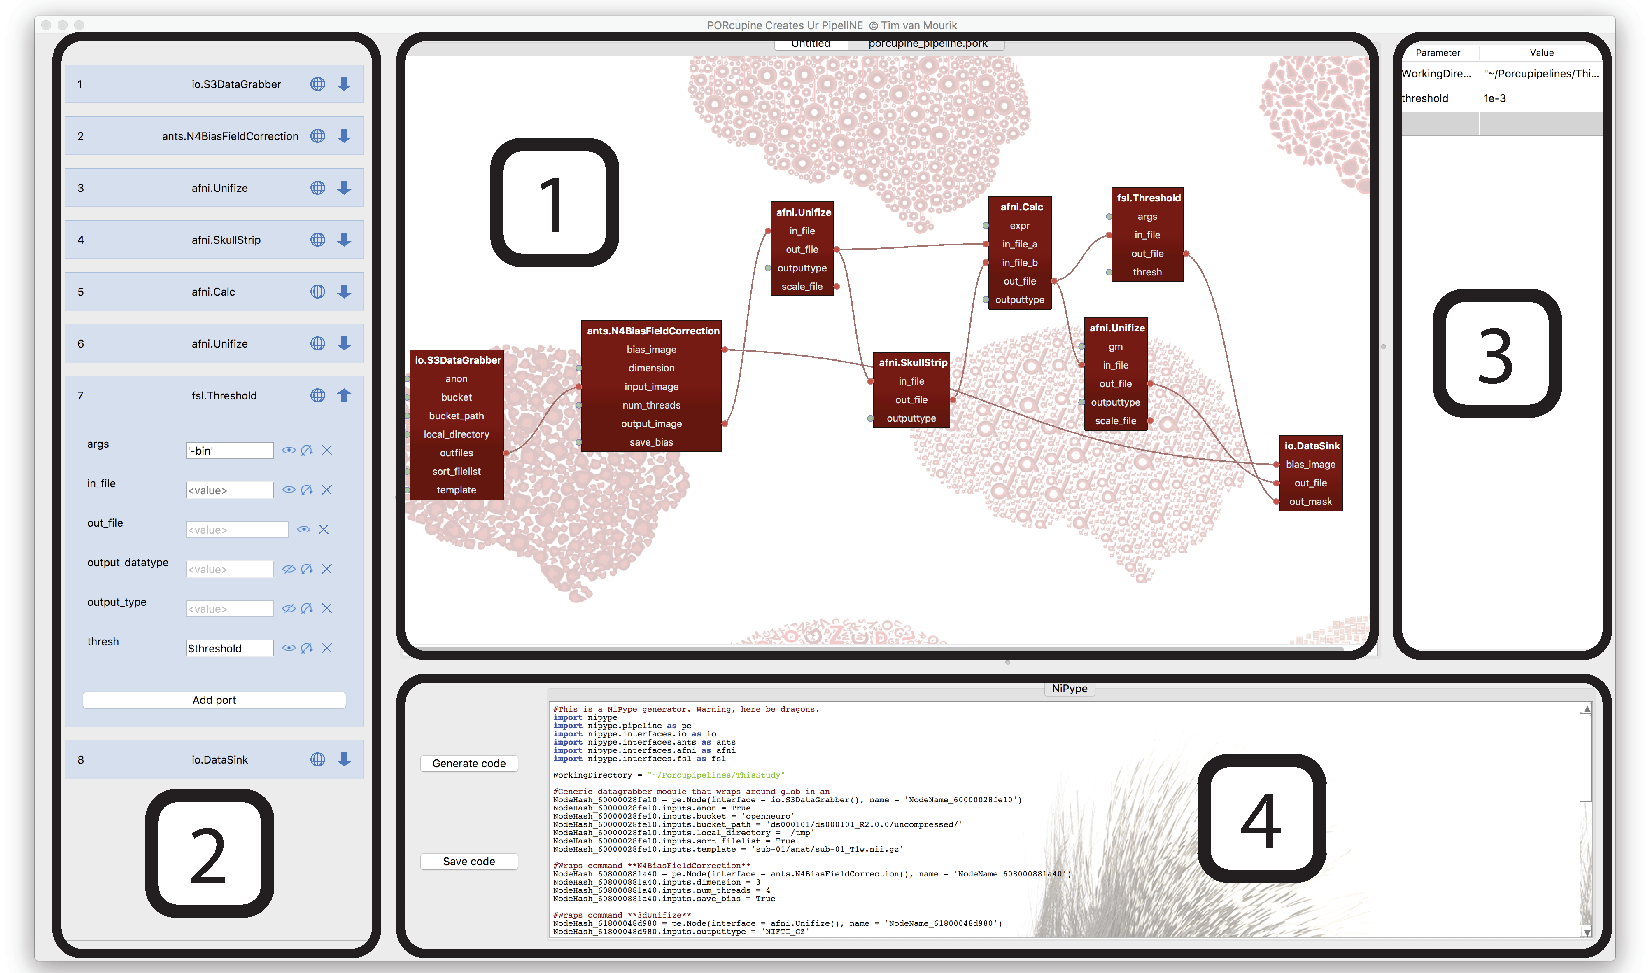
\includegraphics[width=0.9\textwidth, clip=true]{./Chapters/05_Porcupine/./Images/gui_showcase.pdf}
	\caption{A screenshot of a Porcupine workflow. The editor is divided into four panels, each of them targeted at facilitating a more understandable and reproducible analysis. The \emph{workflow editor} (1) provides a visual overview of one's analysis. The functions are all listed in the \emph{node editor} (2), where the parameters for all functions can be orderly stored. This may include links to important parameters that are listed in the \emph{parameter editor} (3), such that an overview of the main analysis settings can be easily viewed and modified. Readily executable analysis code is generated in the \emph{code window} (4)}
	\label{fig:porcupine-editor}
\end{figure}

%scope of this paper
We here focus on code generation that strictly adheres to the Nipype API \cite{Gorgolewski2011}, a Python-based MRI analysis and pipelining package. Nipype is used for its strong focus on uniformity in accessing functions, its link to most major MRI analysis tools, and its emphasis on reproducible science. Porcupine's architecture, however, is in principle agnostic with respect to the specific implementation of the underlying pipelining software. Any package with a consistent interface in the field of e.g. neuroimaging, bioengineering, or astronomy could benefit from using Porcupine's architecture.

%show by example
We first show that we can easily generate a standard fMRI analysis pipeline. After visually dragging and dropping modules, code is automatically created that is usually scripted manually instead. We then show how we facilitate loading data from an online repository, generate a readily executable fMRI pipeline, but also generate a shareable and reproducible analysis environment (using Docker), all with minimal additional effort. This allows for easily scalable analyses that \change{could}{can} be performed locally, but also on computational clusters or with cloud computing, without manual installation of different software packages. 

\subsection{Usage example}
We here show a simple example that constructs a pipeline for a single operation. In three steps, data is loaded, (minimally) processed, and the output is written to disk, as shown in Fig.~\ref{fig:porcupine-simple}. We here show an example that links to an OpenNeuro fMRI data set, but we could load any online data set that is set up according to the BIDS format \cite{Gorgolewski2016}. OpenNeuro's data sets are stored as Amazon repositories (`S3 buckets') and can be loaded by dragging the appropriate module into the workflow editor and typing the name of the bucket into the node editor. Its output can subsequently be connected to a Nipype function node, for example FSL's Brain Extraction Tool. All parameters of the function are listed and can be set in two different ways: either by dragging a link from a previous node's output port to an input port in the next node, or by typing in the parameter in the node editor. Subsequently, output can be written to disk by connecting the desired output to a Nipype DataSink node that collects and stores the data. By pressing the `Generate code` button, the code for this pipeline is automatically generated and can immediately be saved and executed in a Python shell.
\begin{figure}[!ht]
	\centering
	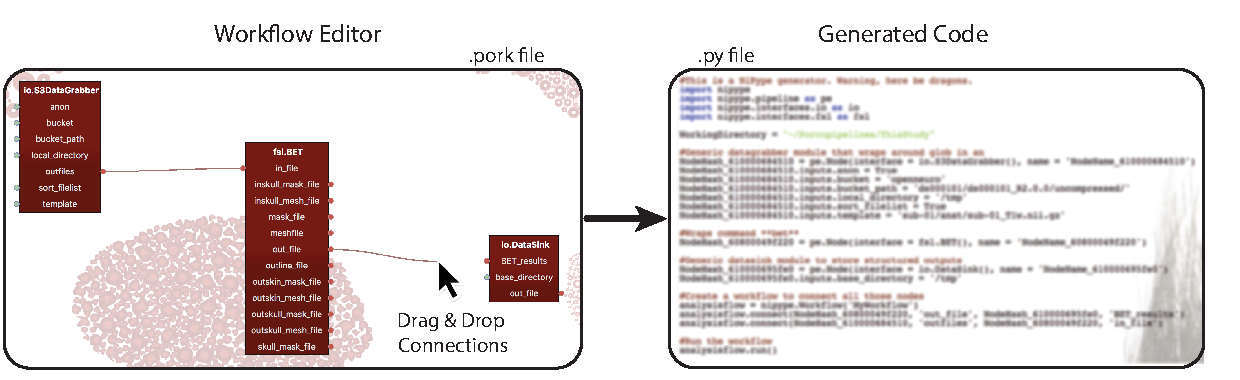
\includegraphics[width=0.9\textwidth, clip=true]{./Chapters/05_Porcupine/./Images/pork_py.pdf}
	\caption{An example of simple workflow. In three steps, this pipeline loads data, processes it, and writes it to disk. This is achieved by connecting the input and output fields from subsequent nodes in the pipeline. The constructed workflow is then transformed in readily executable (Nipype) analysis code.}
	\label{fig:porcupine-simple}
\end{figure}


\subsection{Pipeline sharing}
From a simple example that reads and writes the data, a more complicated pipeline is readily set up. More functionality, i.e. nodes, can be dragged in and connected to quickly build a custom pipeline. As it is commonplace to repeat a single analysis or function for several subjects, sessions, or other variables, every field can be flagged as an `iterator' field. This facilitates looping over variables. Once the pipeline is set up and the code is generated, Nipype offers functionality to construct a visual pipeline graph from custom python code. In Porcupine's proposed use-case, this end point of a standard Nipype pipeline represents the starting point, as shown in Fig.~\ref{fig:porcupine-advanced}. This allows the user to focus on the desired pipeline graph first, and then progress to the manual editing of the generated code.
\begin{figure}[!ht]
	\centering
	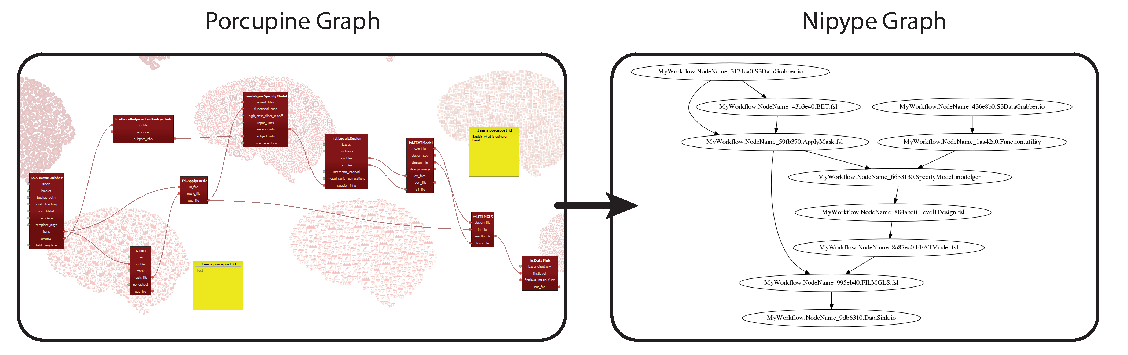
\includegraphics[width=0.9\textwidth, clip=true]{./Chapters/05_Porcupine/./Images/pork_graph.pdf}
	\caption{An example of a more complicated and realistic fMRI preprocessing pipeline. Once the code is generated, this can in turn be transformed into a Nipype graph visualisation. Whereas this is usually the end point for a pipeline in Nipype, we here propose to use a visualisation as a starting point of one's analysis.}
	\label{fig:porcupine-advanced}
\end{figure}

Not only does Porcupine provide a way of setting up a preprocessing  or analysis pipeline, we also provide a means for executing these pipelines in a reproducible environment. In addition to the Python analysis file that is generated, we create a scaffold for a Docker file. Docker (\url{https://www.docker.com}) is an open platform to easily build, run and share applications. The generated Docker file describes a minimal operating system that is required to run the analysis, based on the dependencies of the modules used in the workflow editor. With this Docker file, an image of the full analysis can be built, shared and executed. This provides a simple platform to reproduce results of one's analysis, on the same data set, or on another with only a single change in the data source module. Alternatively, one can use it as a template environment for a new follow-up analysis. As with all generated code, the Docker code is fully customisable to a researcher's need, but our suggested scaffold requires only a single manual edit to be built as a Docker image (see~\nameref{app:docker}). The Docker command will execute the pipeline: load the data from an online repository, process the data, and store only the output data to a local directory. The Docker image includes both the pipeline code and the run environment, and can be shared alongside a paper via DockerHub. The above examples (and many more) as well as extensive documentation and tutorials can be found \href{https://timvanmourik.github.io/Porcupine}{here}.

\subsection{Limitations}
Some features in Nipype have not been implemented. Notably, the JoinNode functionality is not yet accessible from the Porcupine user interface, in which the results from an upstream iterator are aggregated to a single output. Furthermore, custom extensions of Nipype functions are not automatically supported, but we do provide a script to add one's own custom module to Porcupine that would make this functionality accessible. A GUI for this is still an intended point of improvement. In general, feature requests are maintained as \add{\emph{issues} and} \emph{projects} in the \href{https://github.com/TimVanMourik/Porcupine/projects}{GitHub repository}. We encourage people to contribute new ideas or implementations for functionality in terms of modules, new toolboxes, and, most importantly, custom pipelines that can be added to the repository. Details \change{for contributing}{on how to contribute} can be found on the website.

While Porcupine in principle supports all workflow operations, a specific pipeline may well require modules that are not provided within Nipype. It is advised that the user either packages custom code for this into a new module, or manually adds it to the produced code. \change[Reviewer 2]{Porcupine itself functions only as the front-end to the Nipype back-end, but}{We furthermore stress that Porcupine is intended to function as a front-end encapsulation of NiPype, and does not implement the parsing of python files that contain pre-defined nipype pipelines. It also} does not perform type-matching on the input and output of a connection, nor does it perform syntax checking of the manually edited parameters.
\section{Design and Implementation}
Porcupine's graphical user interface was written first with a general visual programming application in mind. The initial interface to Nipype was developed at a three-day coding sprint at BrainHack 2017, Amsterdam. This kickstarted Porcupine in its current form. The source code, as well as the installer files for Windows, Mac, and Linux, are publicly available as a \href{https://github.com/TimVanMourik/Porcupine}{GitHub repository}. Porcupine is free, open source, and released under the GNU General Public License v3.0. \add[Reviewer 1]{It has static digital object identifier (DOI)} \url{doi.org/10.5281/zenodo.1146653}.

Visual programming is a generic way of programming to create a data flow or to perform an ordered task with a modular structure \cite{Myers1986}. Customarily, it allows the user to construct a Directed Acyclic Graph (DAG) \cite{Thulasiraman1992} of conceptualised operations that are subsequently interpreted or compiled as an application \cite{Myers1990}. This format is particularly useful for workflows that fit modular structures, such as most neuroimaging data analyses \cite{Rex2003}. 

\subsection{Architecture}
Not only do we intend researchers to make their analyses (re-)usable and robust, our software also adheres to all 20 simple rules that were laid out to this end \cite{List2017,Taschuk2017}. The updates as well as the releases of the source code are realised by means of a GitHub repository. Installer files are provided for all platforms and do not require administrator privilege. Users are aided in getting started quickly by extensive documentation and an example gallery.

Easy cross-platform installation or compilation was achieved by programming Porcupine as a stand-alone application in Qt Creator (\url{https://www.qt.io}) for C++. Internal file formats were standardised to JSON dictionaries, a format native to Python, Qt, and web applications. This provides a simple means to add new modules to Porcupine, without the need to write additional code. Every dictionary specifies a software package (e.g. `Nipype', `Docker', etc.) that is interpreted by Porcupine and creates code that is native to the package. A package-specific interpreter needs to be written just once, after which new modules that are included in the dictionary will be automatically available in Porcupine.

%the dictionaries
Each JSON dictionary describes a list of functions (internally referred to as 'nodes'). Each function has a name and (optionally) a category, a web url to its documentation, and a block of code. A code block specifies the software package for which the node is meant, the associated piece of code for that function and optionally an additional comment. Furthermore, a node contains any number of data/parameter ports, each of which can be input, output, or both. Optionally, additional flags can be set for ports to be visible in the editor, whether its value is editable, or whether the variable needs to be iterated over. Thus, JSON files for custom nodes can easily be created and added as a dictionary to the graphical interface. We also provide a Python script that converts a custom Python function(s) to a Nipype node dictionary.

\subsection{Extending Porcupine with new toolboxes}
Currently, Porcupine features Nipype and Docker support, but this could easily be extended to other software packages. This requires no major changes to the Porcupine source code, merely the inclusion of a single C++ class that describes the relationship between the nodes, links, and the output code. Specifically, the `CodeGenerator` class must be inherited and has access to the full workflow: the list of nodes, their parameters, and their connections. As long as all functions within an analysis toolbox can be accessed with a consistent interface, they can be represented as modules within Porcupine. Apart from Nipype, support for a laminar specific fMRI analysis toolbox in MATLAB is provided. The developers of the Fastr framework programmed initial support for their code base \cite{Achterberg2016}. Unfortunately, only few neuroimaging packages abide by this uniformity of their functions and hence many cannot be included into Porcupine.

\subsection{Relation to existing pipeline managers}
Porcupine aims to provide an extendable, transparent and flexible platform to build preprocessing and analysis pipelines. Other software packages have made similar attempts at providing visual aids to build or run pipelines. Within neuroimaging, the most notable ones are the JIST pipeline \cite{Lucas2010}, extended with CBS Tools \cite{Bazin2014} and the LONI pipeline \cite{Rex2003}. Porcupine distinguishes itself from these by not creating a run environment, but instead creating the analysis code for the researcher. This retains the possibility of immediately running the code through a Python interpreter, but also creates more flexibility, as researchers can modify and adjust the script according to their needs.\remove[Reviewer 3]{Additionally, as the functions link to existing Nipype interfaces, error reporting is more transparent such that problems can more easily be resolved.} Lastly, our open-source framework is set up to be extendable with new modules within existing frameworks, as well as with completely new frameworks. This provides a future-proof set-up for current and future analysis tools in neuroimaging and perhaps other disciplines.

\section{Availability and Future Directions}
We have presented a new tool to visually construct an analysis pipeline. Subsequently, Porcupine automatically generates the analysis code, and provides a way of running and sharing such analyses. We see this as an important tool and a stepping stone on the path to doing more reproducible and open science. Additionally, this gives researchers a better oversight of their analysis pipeline, allowing for greater ease of developing, understanding, and communicating complex analyses.

Porcupine provides two independent functionalities that dovetail to allow users to more easily take part in reproducible neuroimaging research. They are (1) a graphical user interface for the visual design of analysis pipelines and (2) a framework for the automated creation of docker images to execute and share the designed analysis. 

We anticipate that the ability to design processing pipelines visually instead of programmatically \change{cuts}{will cut} the novice user's learning phase by a considerable amount of time by facilitating understanding and development. The ease of use of a Graphical User Interface (GUI) implementation extends and complements Nipype's flexibility. Thus, it invites researchers to mix and match different tools, and adhere less stringently to the exclusive use of the tools of any given toolbox ecosystem. This flexibility enhances the possible sophistication of processing pipelines, and could for instance be helpful in cross-modal research or multi-site research. Additionally, it may nudge method developers to write new tools in a way that easily integrates with the Nipype and Porcupine structure.

The emphasis that Porcupine puts on visual development of analyses makes it easier to communicate a methods section visually rather than in writing. We foresee that researchers may prefer explicity sharing the created .pork files and the Nipype pipelines that are created from them, instead of solely relying on written descriptions of their methods. Yet another use case for Porcupine is the easy definition of proposed processing workflows for preregistered studies.

Importantly, Porcupine attempts to reduce the steepness of the learning curve that is inherent to the use of complex analysis, by providing a more structured and systematic approach to pipeline creation. It separates the skill of building a conceptual analysis pipeline from the skill of coding this in the appropriate programming language. This places Porcupine in a position to aid in the education of novice neuroimaging researchers, as it allows them to focus on the logic of their processing instead of the creation of the code for the processing - greatly improving and accelerating their understanding of the different steps involved in the preprocessing of neuroimaging data. At the same time, it allows more experienced researchers to spend more time on \change[Reviewer 2]{theconceptual}{the conceptual} side than on implementational side.

Having allowed for the visual design of a pipeline for the preprocessing or analysis of a neuroimaging dataset, the reproducible execution of this pipeline is another step that Porcupine facilitates. By flexibly creating a Docker image tailored to the different preprocessing steps defined visually in the GUI, Porcupine allows the user to share not only the definition of the pipeline but also its execution environment. This step removes the overhead of having to manually install the desired operating system with the matching distribution of MRI analysis software. This final step greatly facilitates the reproducibility of reported results, and is part of a general evolution of the field towards easily shareable and repeatable analyses. 

The generated Docker image can be made High Performance Computing aware \remove{with singularity} by means of dedicated tools such as \href{https://github.com/singularityware/docker2singularity}{docker2singularity}. Alternatively, with only trivial additions to the Dockerfile, it can be transformed into a BIDS app \cite{Gorgolewski2017}. A detailed explanation for doing this can be found on our \href{https://timvanmourik.github.io/Porcupine/documentation/advanced/make-a-bids-app}{website}. An automatic and direct way of creating \add{this} has not yet been implemented. Additionally, integrating support for standardised workflow file formats, such as the Common Workflow Language \cite{Amstutz2016} could further add to Porcupine's aim of reproducibility. Another point of improvement is a functionality to embed pipelines within pipelines. Currently, a complicated pipeline\remove[Reviewer 2]{s} does full justice to the term `spaghetti code', and the number of nodes and links may easily compromise the visual aid in understanding; the very purpose for which Porcupine was created. This may easily be solved by compartmentalising pipelines into logical units by providing an embedded structure.

We intend Porcupine to be a strong aid for doing better, more reproducible and shareable science. By bridging the gap between a conceptual and implementational level of the analysis, we give scientists a better oversight of their pipeline and aid them in developing and communicating their work. We provide extensive and intuitive documentation and a wide range of examples to give users a frictionless start to use Porcupine. We look forward to adding more functionality and\change{support for}{supporting} more toolboxes in the near future.

\section{Supporting information}
\paragraph*{S1 Docker files}
\label{app:docker}
Porcupine provides a Docker image that creates the necessary run time environment for a pipeline that is constructed in the workflow editor. As with all generated code, the Docker code is fully customisable to a researcher's need, but our suggested scaffold requires only a single manual edit to be built as a Docker image. A Docker script can only refer to online or on-disk resources, so the pipeline file needs to be saved manually and added to the Docker file:
\begin{lstlisting}
ADD /path/to/pipeline/script.py /somewhere/porcupipeline.py
CMD ["python", "/somewhere/porcupipeline.py"]
\end{lstlisting}
Once this line is added, the docker image can be built:
\begin{lstlisting}
$ docker build -t mydockerimage -f Dockerfile
\end{lstlisting}
The output from the executed pipeline can be written to a local directory on a researcher's computer (`/my/local/directory') by mounting it to the docker output directory (`/data') with the `-v' option and running the image as if it were a standalone application.
\begin{lstlisting}
$ docker run -v /my/local/directory:/data mydockerimage
\end{lstlisting}
This Docker command will execute the pipeline: load the data from an online repository, process the data, and store only the output data to a local directory. A fully worked out example with detailed explanation can be found \href{https://timvanmourik.github.io/Porcupine/documentation/basics/building-dockerfiles}{here}.
\section{Acknowledgements}
We would like to  thank the organisation of BrainHack Global and BrainHack Amsterdam, specifically Pierre-Louis Bazin, for organising the platform that kickstarted Porcupine in its current form. Tim van Mourik acknowledges support by Spinoza grant SPI 40-118.
\section{Author contributions}
TvM wrote the Porcupine C++ software. TvM, LS, and TK designed the interface to Nipype. LS and TvM built the website. LS wrote the examples and the majority of documentation. TvM, TK, LS, and DGN wrote the paper.

 \afterpage{\blankpage}
 
\chapter{Summary and Discussion}
\chaptermark{Discussion}
\label{ch:discussion}

For long the nature of the processing undertaken by the cortical layers has been recognised as a mystery that needs to be resolved to better understand the computations being performed by our brains \cite{Miller2001}. The most realistic method to date of studying this in living human subjects is with functional MRI, as it it very precise and non invasive. But many challenges in spatial and temporal resolution, resolution, interpretation, and all sorts of noise have to be overcome before this can be easily used to solve neuropsychological problems. The objective of this thesis was to pave the way for doing more routine laminar fMRI analysis. Indeed we made significant steps towards this end. 
We have developed several new methods that solve major problems in laminar analysis, we conducted a full layer specific analysis, and took explicit care to make everything along the way reproducible and reusable. %% <-- unpack

\section*{Chapter 2: Recursive Boundary Registration}
First, we addressed the problem of local distortions that are often present in Echo Planar Images (EPI). Due to inhomogeneities in the main magnetic field, spins in some areas rotate a bit faster or slower than others. Effectively, this causes small shifts of parts of the image with respect to the true position. Thus, even though the true locations of the layers are known, the distortions may easily be larger than the thickness of the layers. Without correcting this effect it is hopeless to get out any reliable layer signal. So that is what we set out to do in Chapter 2.

Geometry transformation from one volume to the other (coregistration) has been very succesful for linear transformations and is used routinely in fMRI analysis. Even on volumes with low resolution, low contrast, or few slices, it may work well \cite{Greve201}, but not for non-linear transformations. Such transformations require a high number of degrees of freedom because of the many parameters that need to be estimated. This leaves much more room for error and therefore usually only works on high contrast data sets. It is used routinely for transforming single subject anatomical space to a template space with the same contrast. However, existing techniques are not powerful enough to undistort low contrast EPI images. We therefore invented a new technique for this, Recursive Boundary Registration. By recursively applying linear transformations on diminishing spatial scales, we effectively compute a non linear registration. In order to guarantee smoothness over all transformations, it is combined with a control point lattice that regulates the transformations. Explicitly taking the geometry of the volume into account as a type of prior knowledge is a novel way to approach non linear registrations.

We tested RBR on two different types of data. First, in order to establish a gold standard, we distorted a FLASH image that is typically without distortion. Because we did this in a controlled manner, we could easily compare the performance of RBR to our ground truth and verify the quality of the registration. We thus proceeded to EPI data set of 11 subjects that had real distortions. As the true size of the distortions was unknown there cannot be an absolute quality metric for the registration. Instead, by adding different levels of noise we showed that there is a clear SNR dependance in the displacement that decreases towards the no-noise condition. Additionally, we provide an abundance of graphical evidence to illustrate the performance of RBR.

The power of the method lies in the fact that it makes explicit use of the gyrification of the brain and the specific geometry of an individual brain. It can therefore get away with little contrast and still produce an accurate registration while preserving the topology of the original. Because of the large number of parameters that needs to be estimated we built in a variety of robustness assurances. Despite the overall improved registration, it is still important to carefully inspect the quality of the registration to verify the required submillimetre accuracy. All in all, this proved to be a valuable tool for preparing Gradient Echo images for subsequent analyses and we use it in our experimental study in Chapter 4. It is now an integral part of the fMRI analysis toolbox for laminar fMRI, \url{https://github.com/TimVanMourik/OpenFmriAnalysis}.

An helpful realisation in developing this method was a more conceptual look on the problem. The problem of coregistration can be classified along two main axes: the type of image contrast can be different or the same, and the required transformation can be linear or non linear. The easiest scenario is to find a linear transformation for a volume with similar contrast. The problem becomes harder when the volume has a different contrast, as the mapping of intensity values from one volume to the next is unknown. If instead the contrast is the same but the required transformation is non linear, it is still solvable to a good approximation \cite{Collins1995}. However, when the contrast is different \emph{and} the registration should be non-linear the, the degrees of freedom of the problem increases drastically, and is not easily estimated anymore. Combine this with the low contrast-to-noise ratio of fMRI data and it is clear that this is a hopeless endeavour with standard volume-to-volume registration. The trick to solve this conundrum is to introduce more prior knowledge to the equation. In this case, we chose to use the geometric information of the cortex and its many gyri and sulci to more accurately estimate a non linear cross-modal registration. This does the trick on a single subject level, but by introducing prior knowledge, we restricted the use cases. Where the previous non-linear transforms could also compute subject-to-template registration, we lost this ability by strictly enforcing equal geometry across volumes. As a general notion, algorithms can become more powerful when they are more specialised. Usually this requires a specific type of prior knowledge in the data that is quantified and optimised.

\section*{Chapter 3: Spatial GLM for laminar fMRI}
Once the geometry of our cortical surfaces is properly aligned with our functional data, there is a next problem: how can the laminar signal be extracted from the MRI volume? There are several intuitive ways. A volume could simply be interpolated at the approximate location of the layers, or classify voxels to be part of it most likely layer. However, it is clear that this inherently smears out the laminar signal to some extent. In Chapter 3 we set out to quantify this signal leakage and to present a new method to reduces it and to more cleanly separate the laminar signal.

We started out with the notion that all voxels are a mixture of a variety of layers. If this mixture could be accurately modeled it could theoretically also be inverted and solved for the layer intensity values by means of the framework of the General Linear Model (GLM). To achieve this, we first set up a mathematical framework to accurately model the layer distribution and subsequently estimate the layer signal intensity. 

Our cortex model incorporates information about the precise location, curvature and thickness of the cortex to model the 



We previously mentioned that methods can become more powerful when they use types of prior knowledge inherent to the data. We here find that this is true, but might come at the cost of a la

The prior knowledge 


Due to the many factors that could play a role in the 
The combinatoric explosion of the many dimensions

\section*{Chapter 4: Layer Specificity in Visual Attention}


"In addition, excitatory neurons may quickly redistribute input from the thalamus by means of their local axonal collaterals, 
so that cortical activity nearly instantaneously spreads over several layers and columns to mediate perception of sensory stimuli (Reyes-Puerta et al., 2015)"

publication bias 
null result


\section*{Chapter 5: Pipelines for fMRI with Porcupine}






\linespread{1.5}
\newpage
 \afterpage{\blankpage}
 \chapter{Appendix}
\chaptermark{Appendix}
\thispagestyle{empty}
\bibliographystyle{abbrv}
\renewcommand{\bibsection}{\section{Bibliography}}
\bibliography{Bibliography/Bibliography}

\newpage
\section{Nederlandse samenvatting}
In dit proefschrift zoomen we zo ver mogelijk in op het brein, en proberen we een glimp op te vangen van de processen die daar plaatsvinden. Door iedere paar seconden een driedimensionale afbeelding te maken van het brein kunnen we een indruk krijgen wat er zich daar afspeelt. Op een grove schaal kunnen we zien welke breingebieden actief worden bij verschillende taken: als het licht aangaat, wordt de achterkant van je brein actief (de \emph{visuele cortex}), en voornamelijk de linker zijkant van het brein (je taalcentrum) wordt actief als je deze tekst leest. Maar wat betekent het dat die gebieden actief worden? Wat doen ze dan precies? Op een MRI-scanner kunnen we voornamelijk zien dat gebieden meer of minder zuurstof verbruiken. Dat vertelt echter niet zo gek veel over het proces wat zich daar afspeelt. Om daar iets beter achter te komen, moeten we nog verder kijken. Dankzij anatomische ontledingen van het brein weten we dat de buitenste schil van het brein, de grijze stof, uit verschillende laagjes bestaat. Sommige lagen ontvangen informatie en sommige lagen sturen het door naar de andere breingebieden. Het doel van dit proefschrift is de functie van verschillende lagen te laten zien op basis van MRI-scans.

Dat is echter niet makkelijk: de laagjes zijn zo klein dat de resolutie van de MRI-scanner maar ternauwernood goed genoeg is. En daar komt nog bij dat de plaatjes die uit een MRI-scanner komen zelf ook licht verschoven zijn. Vervolgens moet je erachter zien te komen hoe, in een kronkelend brein, de laagjes precies verdeeld zijn over alle volume-pixels (voxels) van het driedimensionale plaatje. En verder wilden we dit niet gewoon \'e\'en keer uitvoeren, maar zorgen dat iedereen dit type onderzoek voortaan ook kan doen.

% hoofdstuk 2
In \textbf{hoofdstuk 2} zijn we begonnen met het eerste probleem: binnen de afbeeldingen die uit de MRI-scanner komen, liggen de verschillende lagen niet exact op de goede plek. Dit heeft te maken met de manier waarop een MRI-scanner werkt: in het midden van scanner wordt een groot magneetveld gecre\"eerd wat cruciaal is voor het maken van scans. Echter, als het magneetveld niet exact homogeen is, vertaalt dit zich in de scan als kleine (lokale) verplaatsingen. Omdat het nou juist cruciaal is tot op het kleinste niveau op de goede plek te meten als je de verschillende lagen wil meten, is dit een groot probleem. Daarom hebben we een methode bedacht om de scan `recht te trekken' en weer terug op de goede plek te leggen. Op basis van beeldanalyse kijken we heel precies waar de grenzen van de witte en grijze stof zitten, ten opzichte van een niet verplaatste referentie scan. We laten vervolgens op verschillende data sets zien dat de methode daadwerkelijk een veel preciezer beeld geeft over de locatie van de verschillende lagen. 

% hoofdstuk 3
Hiermee is de locatie van de lagen met hoge precisie bekend. Het hele hersenoppervlak ligt echter nog steeds gekronkeld in het volume en de verschillende lagen zijn zo klein dat ze nog niet duidelijk te zien zijn. In \textbf{hoofdstuk 3} beschrijven we een nieuwe methode op basis waarvan de signalen uit verschillende lagen beter geschat kunnen worden. Dit doen we door middel van een wiskundig model dat beschrijft hoe de laagjes verdeeld zijn over het volume. Aan de hand van dit model kunnen we preciezer dan voorheen de signalen uit de lagen halen. Op basis van drie verschillende datasets laten we zien hoe deze nieuwe methode presteert. In een simulatie van een MRI-volume blijkt het veel beter te werken dan bestaande methode. Dit is echter niet zo duidelijk in data van echte scans. De reden hiervoor is dat onze methode op goede data inderdaad een betere schatting kan maken, maar wel gevoeliger is voor ruis in de data. Dat maakt het moeilijk goed zicht te krijgen op het verschil tussen de methodes op standaard MRI-scans.

% hoofdstuk 4
Na deze twee methodologische studies om de weg vrij te maken voor laag-specifieke analyse, hebben we in \textbf{hoofdstuk 4} geprobeerd uit te zoeken of de lagen inderdaad verschillende activatie tonen bij verschillende processen. Hiervoor hebben we een aandachtstaak gebruikt. We vroegen mensen hun aandacht links of rechts te focussen en af en toe verscheen er een stimulus (een zwart-wit gestreept plaatje) op het scherm. Zo wilden we onderzoeken of het effect van aandacht in andere lagen te zien valt dan het effect van het zien van een stimulus. Op brein niveau was er wel degelijk een effect te merken, maar op laagniveau zagen we geen verschil. Dit is dus een nul-resultaat met betrekking tot de signalen uit de verschillende lagen. Het is moeilijk te zeggen wat hier precies de reden van is: of het effect niet bestaat, of het effect niet sterk genoeg was, of dat de methodes niet goed genoeg waren om het eruit te halen (of een combinatie van factoren).

% hoofdstuk 5
\textbf{Hoofdstuk 5} gaat over een applicatie die we ontwikkeld hebben om het makkelijker te maken om MRI data te analyseren, Porcupine. Analyses bestaan doorgaans uit lange scripts die een aaneenschakeling beschrijven van verschillende bewerkingen die uitgevoerd moeten worden op de gemeten data. Onderzoekers schrijven deze analyse code vaak zelf, maar deze scripts zijn vaak moeilijk te interpreteren. In plaats hiervan kan een analyse in Porcupine visueel geprogrammeerd worden door blokjes aan elkaar te verbinden. Dit representeert de volgorde van de analysestappen en laat zo op een grafische manier zien hoe de `workflow' eruit ziet. Porcupine genereert vervolgens de analyse code die direct uitgevoerd kan worden. Omdat dit een inzichtelijke weergave biedt die makkelijker deelbaar is en makkelijker valt aan te passen dan huidige analyse scripts, zorgt dit voor een reproduceerbaardere wetenschap.

% Concluding remarks
Hiermee maakt het werk in dit proefschrift de weg vrij om de lagen van de cortex meer routinematig te analyseren. Alhoewel we in dit onderzoek geen effecten gevonden hebben, lijken andere studies (die dezelfde methodes hebben gebruikt) wel resultaten op te leveren. Het is dus nog onduidelijk wat voor informatie er precies te vinden is als we met die precisie in het brein proberen te kijken. Laag-specifieke brein analyse in functionele MRI staat hiermee dus nog in de kinderschoenen, en onze methodologische ontwikkelingen staan hieraan ten grondslag.





\newpage
\section{Biography}
\addcontentsline{toc}{chapter}{Biography}
Tim van Mourik was born on September 27th 1990 in Leiden, the Netherlands. After graduating from the Stedelijk Gymnasium Leiden, he went on to pursue a Bachelor's degree in the exact sciences at the Roosevelt Academy (currently: University College Roosevelt). After this, he enrolled in the Master Computer Animation and Visual Effects at Bournemouth University. Over the course of this program, he started to develop an interest in medical image processing and completed the program with an internship at the Donders Centre for Cognitive Neuroimaging under the supervision of prof. David Norris. As MRI scanners operate on physical and mathematical principles, subsequently producing three-dimensional images, this perfectly combined Tim's expertises and interests. He continued to work as a research assistant at the Donders Institute where he was initiated in the world of neuroimaging and laminar analysis. In February 2014, he started a four-year PhD project to investigate and better understand the cortical layers of the brain. During this time he developed methods for better analysing laminar fMRI data and under the supervision of Dr. Janneke Jehee, he conducted a study on the layer specificity of spatial attention. All tools, code, and data for his published work is openly available, as Tim is a strong proponent of open science, data and code sharing, and open source development. In this spirit, he programmed worfklow software, Porcupine, that automatically and more transparently creates analysis code. He is currently contuining this line of work by creating an online platform for easier data sharing, GiraffeTools. It is unknown where he acquired his peculiar taste for silly acronyms. For these efforts towards open science he was elected to be the chair of the Open Science Room at OHBM 2019, Rome. 

\newpage
\section{Author publications}

\subsection{Published papers}

\hangindent=2em
\noindent
% Author
\textsc{\textbf{T.~van Mourik}, L.~Snoek, T.~Knapen, and D.~Norris.} 
% Year
(2018).
% Title
Porcupine: a visual pipeline tool for neuroimaging analysis.
% Journal
\emph{PLoS computational biology.}


\hangindent=2em
\noindent
% Author
\textsc{S.~Lawrence, \textbf{T.~van Mourik}, P.~J. Koopmans, D.~Norris, and F.~de~Lange.} 
% Year
(2018).
% Title
Laminar Organization of Working Memory Signals in Human Visual Cortex. 
% Journal
\emph{Current Biology, in press.}


\hangindent=2em
\noindent
% Author
\textsc{N.~Z.~Bielczyk, S.~Uithol, \textbf{T.~van Mourik}, P.~Anderson, J.~C.~Glennon, and J.~K.~Buitelaar} 
% Year
(2018).
% Title
Disentangling causal webs in the brain using functional Magnetic Resonance Imaging: A review of current approaches.
% Journal
\emph{Network Neuroscience.}


\hangindent=2em
\noindent
% Author
\textsc{R.~Scheeringa, P.~J.~Koopmans, \textbf{T.~van Mourik}, D.~Norris, and Jensen.} 
% Year
(2016).
% Title
The relationship between oscillatory {EEG} activity and the laminar-specific bold signal.
% Journal
\emph{PNAS.}


\hangindent=2em
\noindent
% Author
\textsc{P.~Kok, L.~Bains, \textbf{T.~van Mourik}, D.~Norris, and F.~de~Lange.} 
% Year
(2016).
% Title
Selective activation of the deep layers of the human primary visual	cortex by top-down feedback.
% Journal
\emph{Current Biology.}


\hangindent=2em
\noindent
% Author
\textsc{M.~Kleinnijenhuis, \textbf{T.~van Mourik}, D.~G. Norris, D.~J. Ruiter, A.-M. van	Cappellen~van Walsum, and M.~Barth.} 
% Year
(2015).
% Title
Diffusion tensor characteristics of gyrencephaly using high	resolution diffusion {MRI} in vivo at 7{T}.
% Journal
\emph{NeuroImage.}



\subsection{Publications in preparation}

\hangindent=2em
\noindent
% Author
\textsc{\textbf{T.~van Mourik}, P.~J. Koopmans, L.~J. Bains, D.~G. Norris, and J.~F. Jehee.} 
% Title
Investigation of layer specific bold during visual attention in the human visual cortex.
% Journal
\emph{In preparation.}


\hangindent=2em
\noindent
% Author
\textsc{\textbf{T.~van Mourik}, P.~J. Koopmans, L.~J. Bains, and D.~G. Norris.} 
% Title
Improved cortical boundary registration for locally distorted fMRI scans.
% Journal
\emph{Submitted, Preprint on bioRxiv.}


\hangindent=2em
\noindent
% Author
\textsc{\textbf{T.~van Mourik}, J.~P.~J.~M.~ van der Eerden, P-L.~Bazin, D.~G. Norris.} 
% Year
(2018).
% Title
Laminar signal extraction over extended cortical areas by means of a spatial GLM.
% Journal
\emph{Submitted, Preprint on bioRxiv.}


\hangindent=2em
\noindent
% Author
\textsc{F.~Molaei-Vaneghi, N.~Zaretskaya, \textbf{T.~van Mourik}, J.~Bause, K.~Scheffler, and A.~Bartels.} 
% Title
9.4 T Human fMRI Study Reveals that Real World Motion Perception Does Not Involve Laminar Organization in V1 and V5/MT.
% Journal
\emph{Submitted.}


\hangindent=2em
\noindent
% Author
\textsc{S.~H.~P.~Collin, P.~van den Broek, \textbf{T.~van Mourik}, P.~Desain, C.~F.~Doeller.}
% Title
Creating an artificial memory context alters associative memory formation.
% Journal
\emph{In preparation.}

\newpage
\section{Acknowledgements}

Over the six years that I spent working at the Donders Institute I have met so many people without whom this thesis would not be what it is today. I cannot do justice to of you but I will at least try for a small subset.

%%%%%% David
First, I would like to thank my supervisor, promotor David Norris. When I came in as a student of the exact sciences I preferred to put \emph{quod erat demonstrandum} at the end of every paragraph. You taught me a lot about the scientific method in neuroscience, bigger pictures and the gran(d/t) scheme of things, the politics of laminar analysis, and much more. Our Bert and Ernie roles that we took on in meetings for me lead to more out-of-the-box thinking and I hope that I managed to form them into pragmatic and realistic solutions. I am thankful for the way in which you stay close to the real science and the amount of dedication and personal attention you give to your students, while still having them to express their autonomy to become an independent researcher.

%%%%%% Janneke
I would especially like to thank my co-promotor Janneke Jehee. Visual computation, so I found out, has nothing to do with visual effects, and also not so much with computers. My very first email to the Donders Institute was to inquire about a position in your lab. But you kindly explained that the computations of the visual cortex might not suit my interest or skillset and referred me to the head of the MR physics lab. It was years later that our paths crossed again when you took me up in your lab when I wanted to study layers in the visual cortex. I am very grateful for the time and dedication with which you helped me conduct this study from beginning to (pending) end. I truly admire your dedication, resilience, and extreme precision with words, analysis, and way of doing science. The time that I spent in your lab has hooked me to the workings of the visual cortex, but it has certainly broadened my horizon, made me a better scientist, for which I am very grateful.

%%%%%% The FAD
When I started as a research assistant, there was still a dedicated culture of Friday Afternoon Drinks. From the very first week on, this made me feel welcome at the Donders and familiarised me in no time with all restaurants in Nijmegen and Romagna. And fortunately it was not all too often that this resulted in knife fights over a glass of white wine. Although the old gang has left the building (save some Donders dinosaurs), but the FAD still remains, and I would like to thank everybody with whom I have conversations and discussion to brighten up my Friday afternoon.

%%%%%% The Kitchen
Thanks to everybody in the kitchen, the old kitchen and the new canteen, for a countless number of lunches, coffees, random cake days (and those rare random suit-up days), and much more. Whether the topic of the day was general linear models, the state of science, of the world, of Brexit, or just pink elephants and the order of the day, I appreciated the diverse and stimulating environment. Over the last six years the Donders grew out from a village to a city, with all its infrastructural perks, but without the `market square' like atmosphere in the kitchen. ``Having only a single, slow coddee machine in a research institute is an underappreciated method for enhancing interdisciplinary collaboration'' (Mostert 2016).

%%%%%% Lab group
I would like to thank my lab group for the feedback on layers and porcupines, for sharing frustrations over rejection in the info-meeting, and for the historical geo-political discussion in the group lunches.

%%%%%% Office mates
Thanks to all office mates that I had over the years. For the company, the \emph{boekje-bijna-klaar?} encouragements, sharing in the MATLAB frustrations, the Armin moments on Friday afternoon (before the FAD of course), and much more. 
 
%%%%%% Admin
The backbone of the Donders is formed, of course, by Tildie, Ayse and the administration, Marek and the minions, and `koning-van-de-kelder' Paul. Thank you for all the help and support, and making everything run smoothly. We all know that the Donders would collapse without you. 

%%%%%% Vierkant
There is always one special week per year reserved for Vierkant, the maths puzzle camp. Thanks to all Vierkanters for this exciting and stimulating week, for the random sketches, for each one of you to bring your own kind of crazyness along. 

%%%%%% Paranymphs & family 
Thanks to my dear paranymphs, Tom, Jelle, and Annelies, for all the support along the way. Not just for the home stretch, but primarily in all the preceding years. You have been a sounding board for many a wonky idea that eventually made it to this thesis. A special thanks to my family, who may not always have understood what I have been doing all these years, but still unconditionally supported doing it.

%%%%%% Tineke
Dear Tineke, my Queen of Hearts, occupational panda and occasional sloth. Acronym expert, kindest supporter, and toughest critic. It is quite unclear where we will end up next, but it will be somewhere together. 





\newpage

\section{Donders Graduate School for Cognitive Neuroscience}

For a successful research Institute, it is vital to train the next generation of young scientists. To achieve this goal, the Donders Institute for Brain, Cognition and Behaviour established the Donders Graduate School for Cognitive Neuroscience (DGCN), which was officially recognised as a national graduate school in 2009. The Graduate School covers training at both Master's and PhD level and provides an excellent educational context fully aligned with the research programme of the Donders Institute.

The school successfully attracts highly talented national and international students in biology, physics, psycholinguistics, psychology, behavioral science, medicine and related disciplines. Selective admission and assessment centers guarantee the enrolment of the best and most motivated students.

The DGCN tracks the career of PhD graduates carefully. More than 50\% of PhD alumni show a continuation in academia with postdoc positions at top institutes worldwide, e.g. Stanford University, University of Oxford, University of Cambridge, UCL London, MPI Leipzig, Hanyang University in South Korea, NTNU Norway, University of Illinois, North Western University, Northeastern University in Boston, ETH Z\"urich, University of Vienna etc. Positions outside academia spread among the following sectors: specialists in a medical environment, mainly in genetics, geriatrics, psychiatry and neurology. Specialists in a psychological environment, e.g. as specialist in neuropsychology, psychological diagnostics or therapy. Positions in higher education as coordinators or lecturers. A smaller percentage enters business as research consultants, analysts or head of research and development. Fewer graduates stay in a research environment as lab coordinators, technical support or policy advisors. Upcoming possibilities are positions in the IT sector and management position in pharmaceutical industry. In general, the PhDs graduates almost invariably continue with high-quality positions that play an important role in our knowledge economy.

For more information on the DGCN as well as past and upcoming defenses please visit: 

\url{https://www.ru.nl/donders/graduate-school/phd}




 \afterpage{\blankpage}

\end{document}
